%!TEX root = ../dissertation.tex
\begin{savequote}[75mm]
Tough part.
\qauthor{Revolutionaries.}
\end{savequote}

\chapter{Background Estimation}

\section{Background composition}
Backgrounds of this analysis are mostly QCD multijet events and \ttbar events. \ttbar cross section increased by a factor of \href{https://cds.cern.ch/record/2227057/files/STDM-2016-02-02.pdf}{3.4}.


\section{Sideband Region Distributions}


\section{Control Region Distributions}

\paragraph{}
This section shows comparisons of data with the prediction of QCD multi-jets and \ttbar in the control region (CR), which is identical to the signal region (SR) except the large-$R$ jets are required to have masses close but not too close to the Higgs mass. The definition can be seen in Section~\ref{sec:boosted-SBCR}. The predicted and observed event yields are summarized in Tables~\ref{tab:yields4b} and~\ref{tab:yields3b}.

Figures~\ref{fig:boosted-4b-control-ak10-lead}, \ref{fig:boosted-4b-control-ak10-subl}, \ref{fig:boosted-4b-control-ak2}, and \ref{fig:boosted-4b-control-ak10-system} show predictions of various kinematics of the large-$R$ jets and their associated track jets in the 4$b$ selection. The shapes and normalization are a feature of the prediction, where the normalization is derived in the SB. The quality of the prediction is generally good, and no clear systematic biases are observed.

Figures~\ref{fig:boosted-3b-control-ak10-lead}, \ref{fig:boosted-3b-control-ak10-subl}, \ref{fig:boosted-3b-control-ak2},  and \ref{fig:boosted-3b-control-ak10-system} show predictions of various kinematics of the large-$R$ jets and their associated track jets in the 3$b$ selection. The shapes and normalization are a feature of the prediction, where the normalization is derived in the SB. The quality of the prediction is generally good, and no clear systematic biases are observed.

Figures~\ref{fig:boosted-2bs-control-ak10-lead}, \ref{fig:boosted-2bs-control-ak10-subl}, \ref{fig:boosted-2bs-control-ak2},  and \ref{fig:boosted-2bs-control-ak10-system} show predictions of various kinematics of the large-$R$ jets and their associated track jets in the 2$bs$ selection. The shapes and normalization are a feature of the prediction, where the normalization is derived in the SB. The quality of the prediction is generally good, and no clear systematic biases are observed.

\begin{figure*}[htbp!]
\begin{center}
0.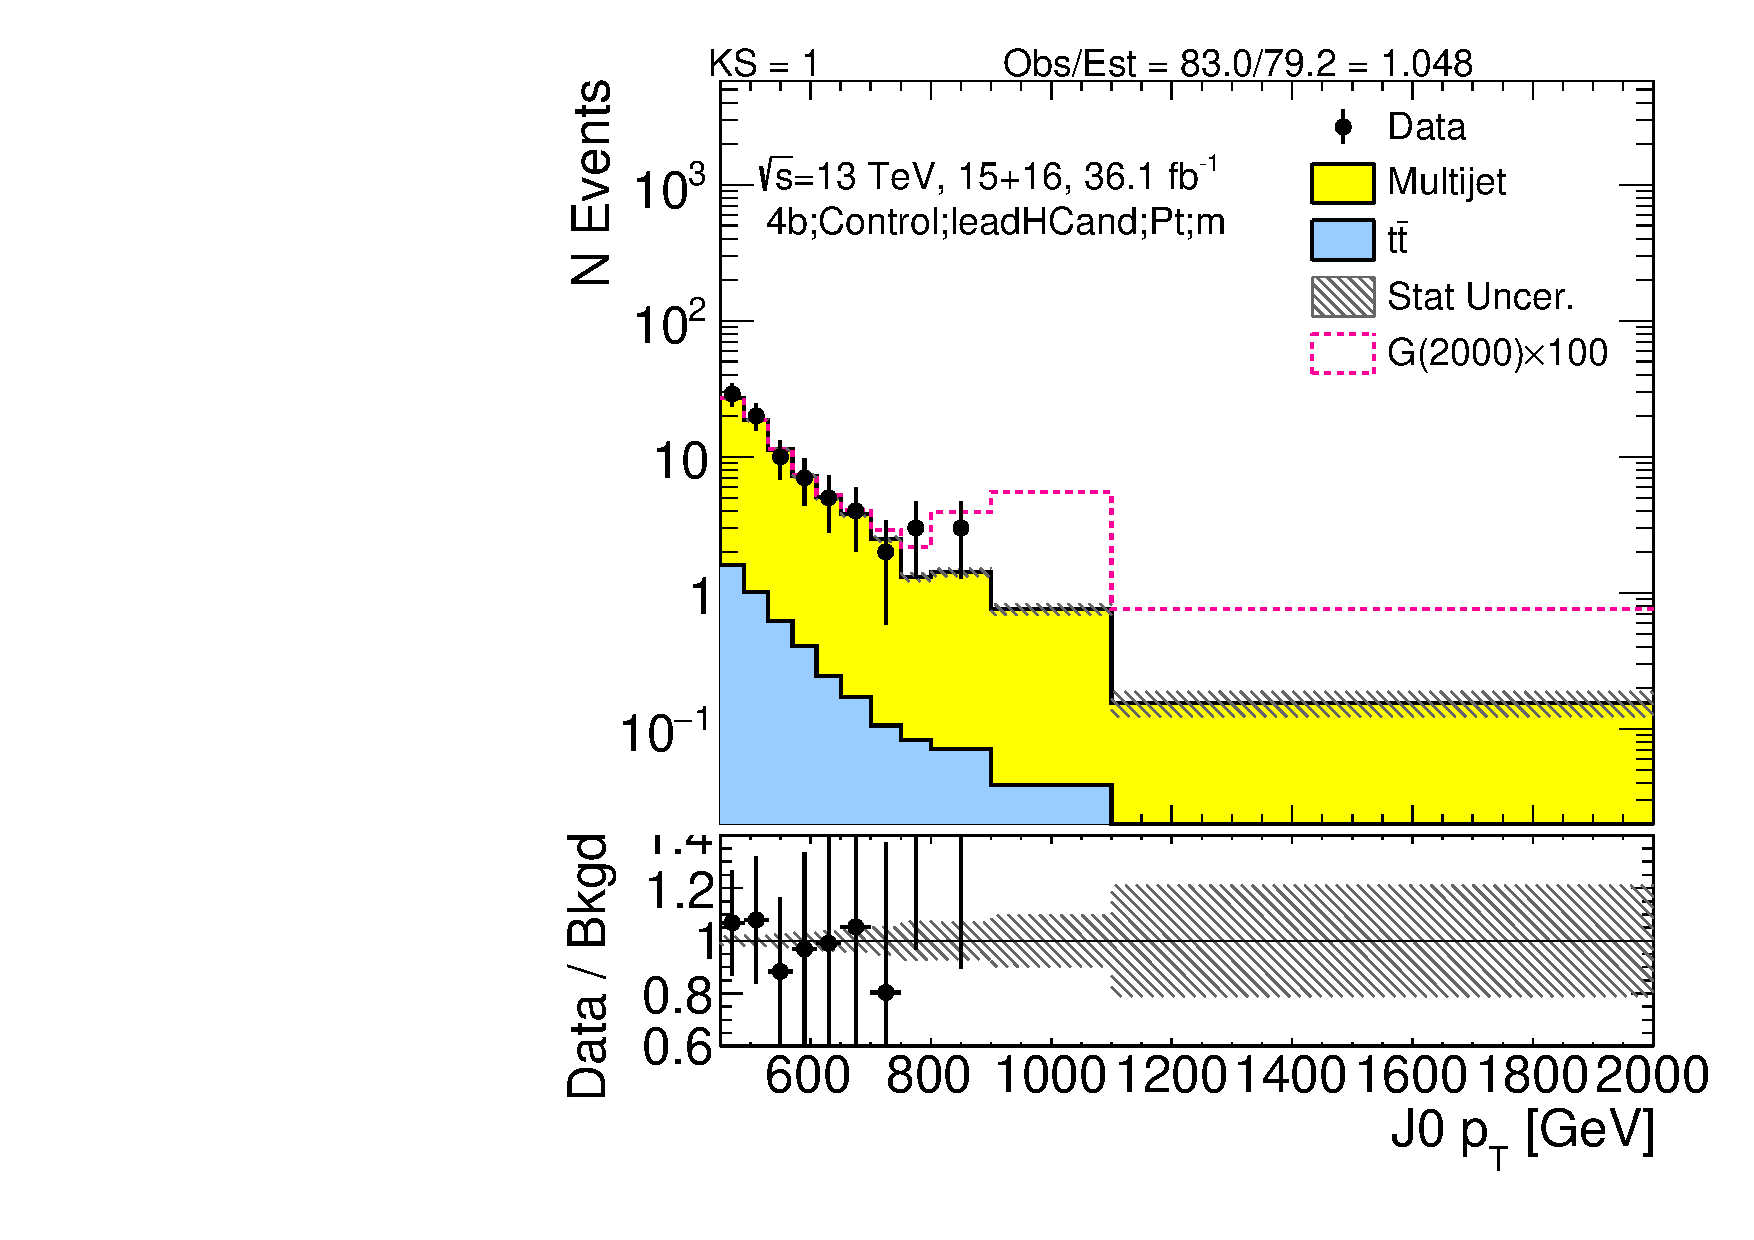
\includegraphics[width=0.33\textwidth, angle=270]{./figures/boosted/Control/Moriond_FourTag_Control_leadHCand_Pt_m_1.pdf}
0.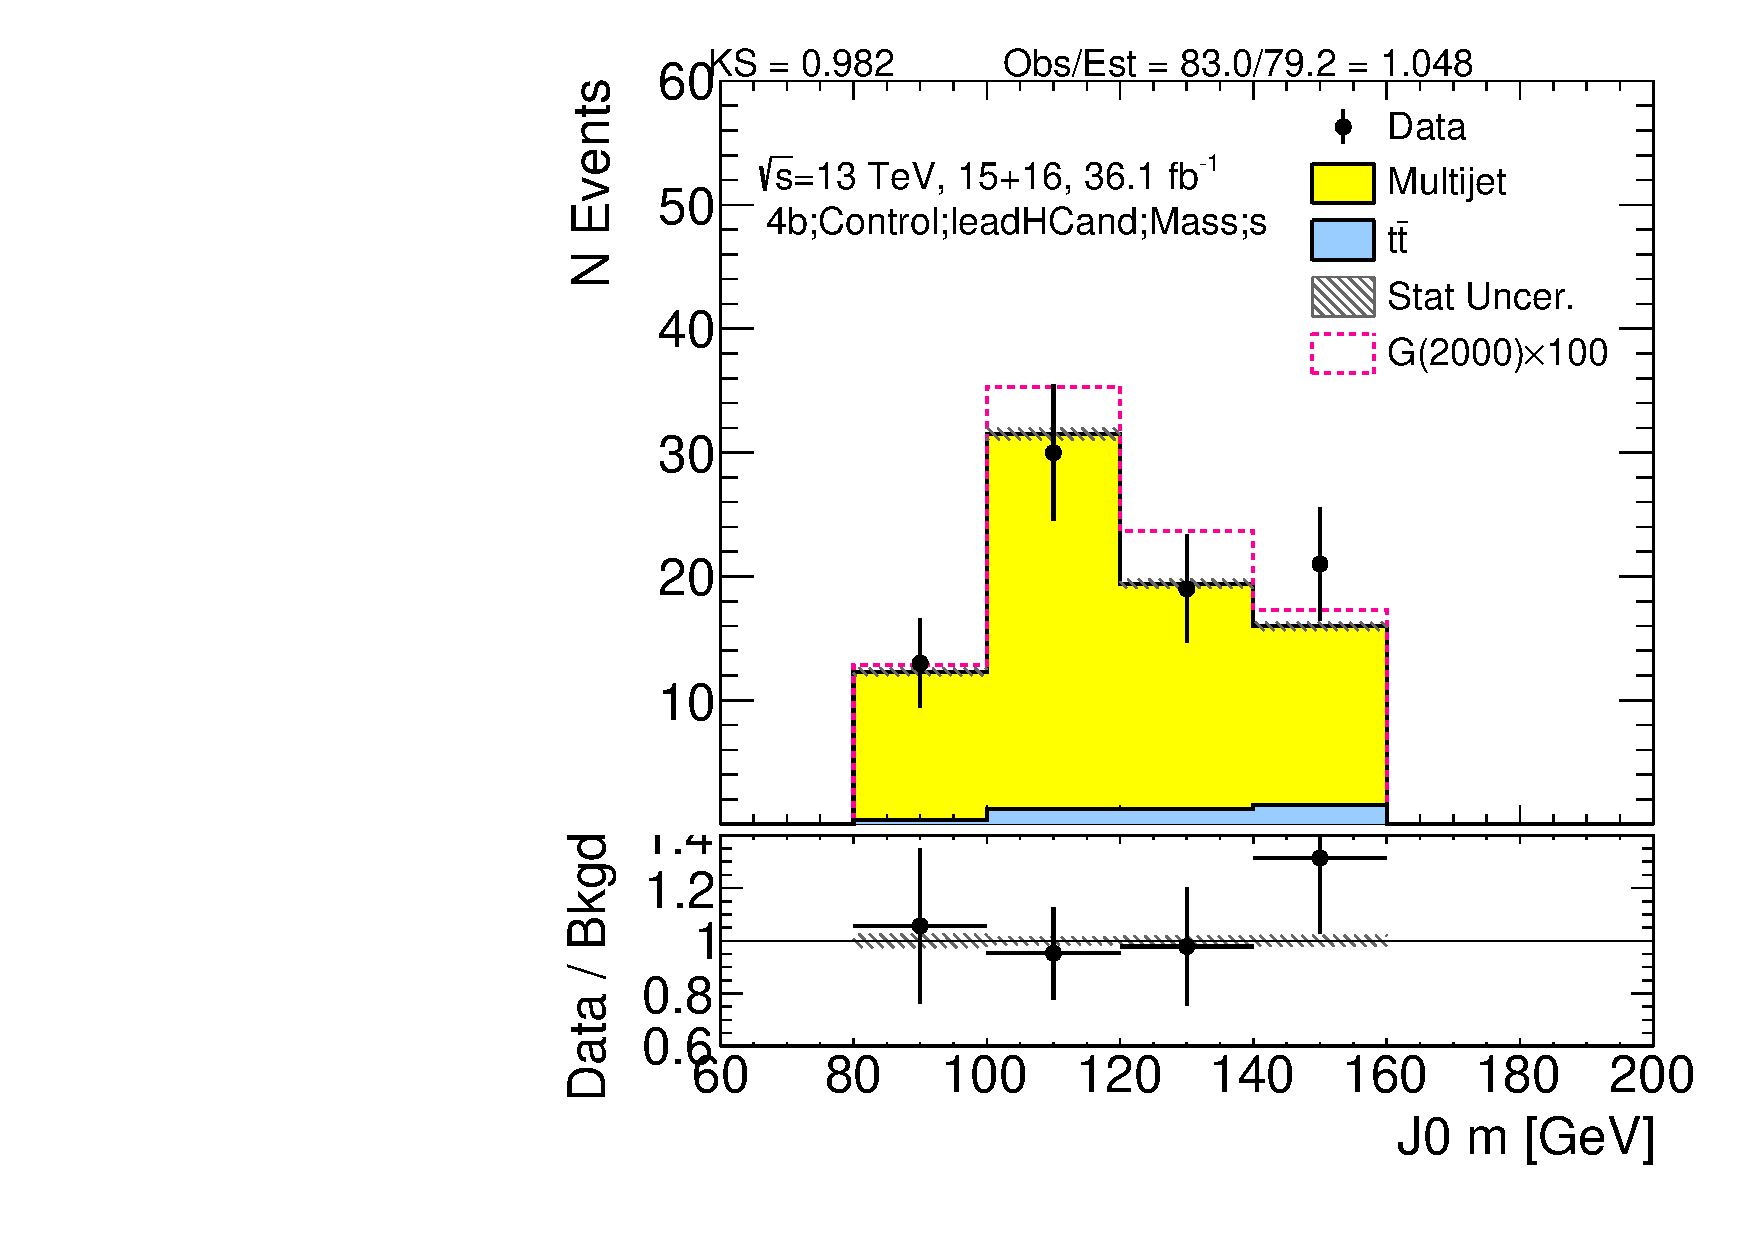
\includegraphics[width=0.33\textwidth, angle=270]{./figures/boosted/Control/Moriond_FourTag_Control_leadHCand_Mass_s.pdf}\\
0.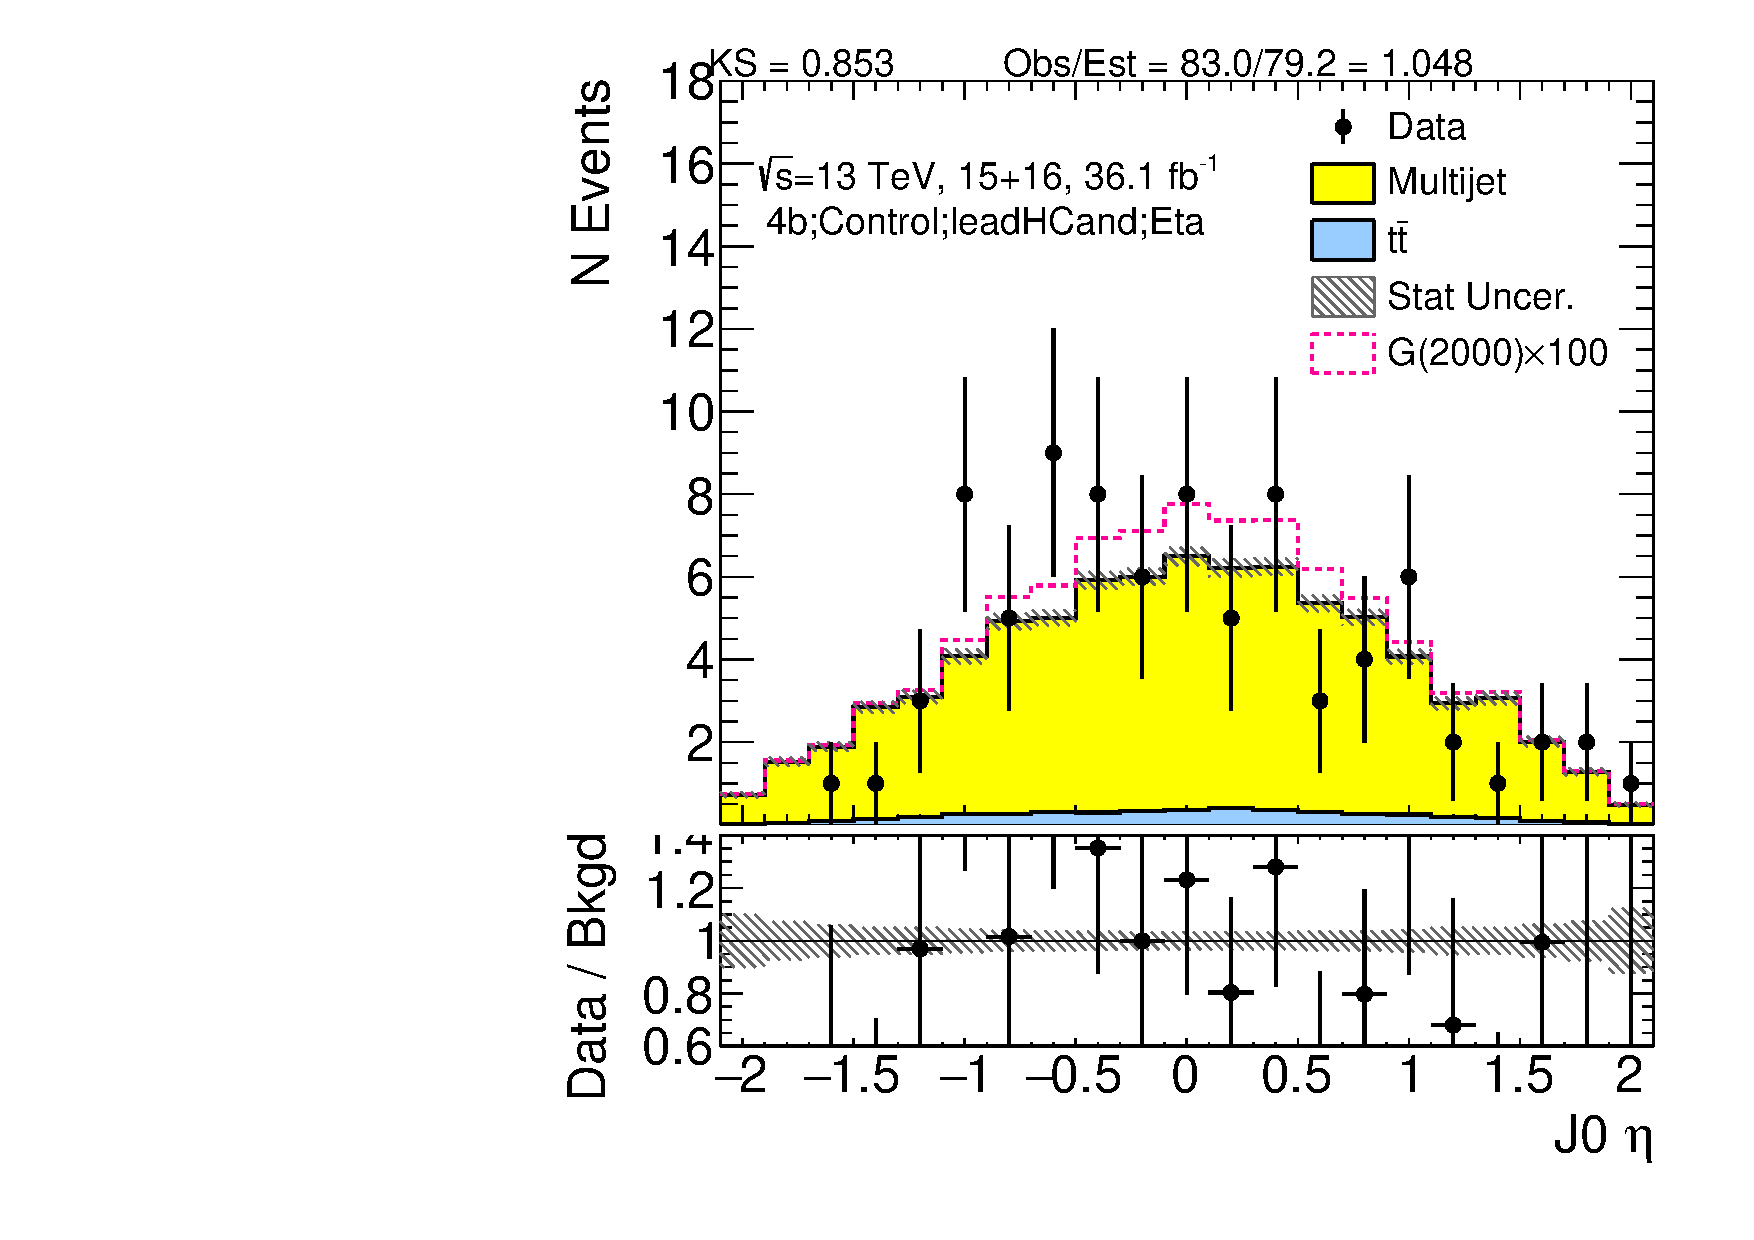
\includegraphics[width=0.33\textwidth, angle=270]{./figures/boosted/Control/Moriond_FourTag_Control_leadHCand_Eta.pdf}
0.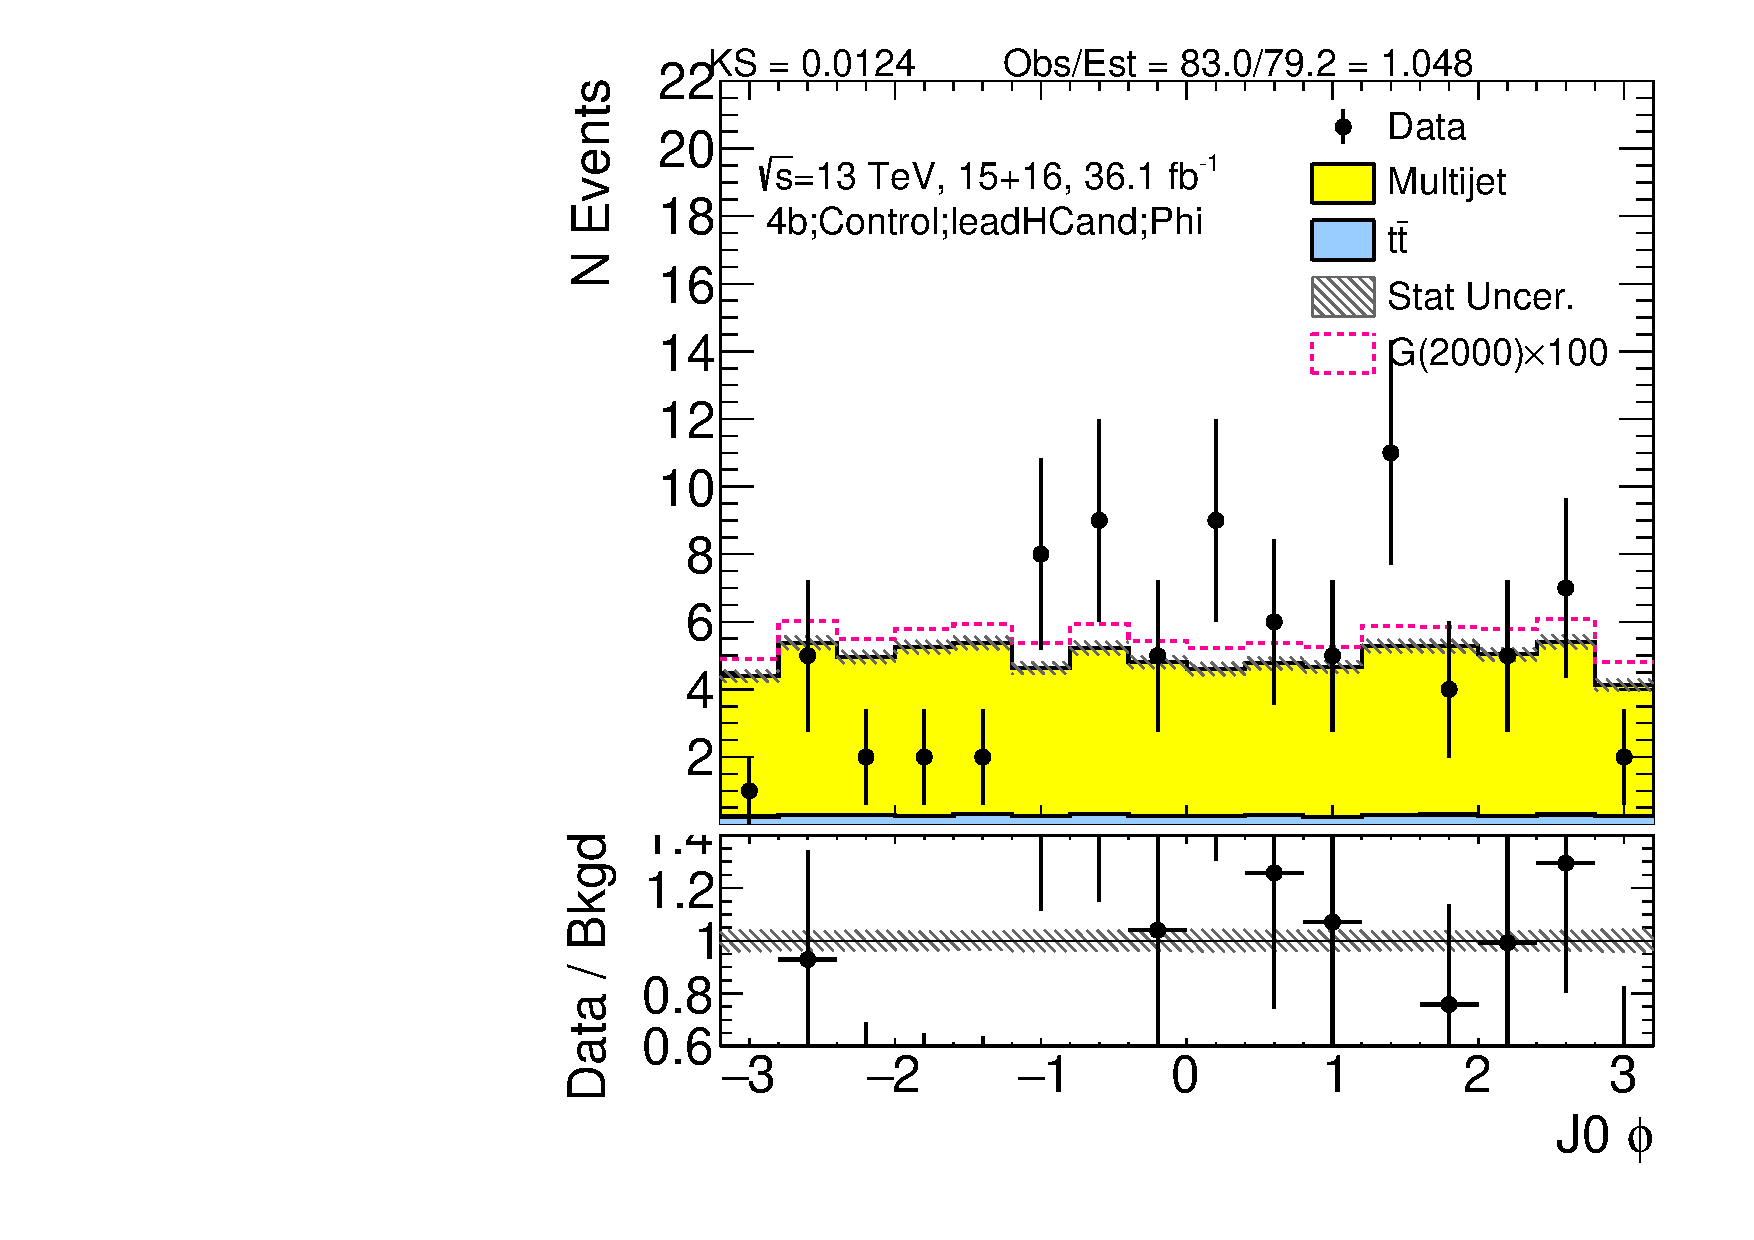
\includegraphics[width=0.33\textwidth, angle=270]{./figures/boosted/Control/Moriond_FourTag_Control_leadHCand_Phi.pdf}
  \caption{Kinematics of the lead large-$R$ jet in data and prediction in the sideband region after requiring 4 $b$-tags. The normalization agrees by construction, and the shapes are a feature of the prediction.}
  \label{fig:boosted-4b-control-ak10-lead}
\end{center}
\end{figure*}

\begin{figure*}[htbp!]
\begin{center}
0.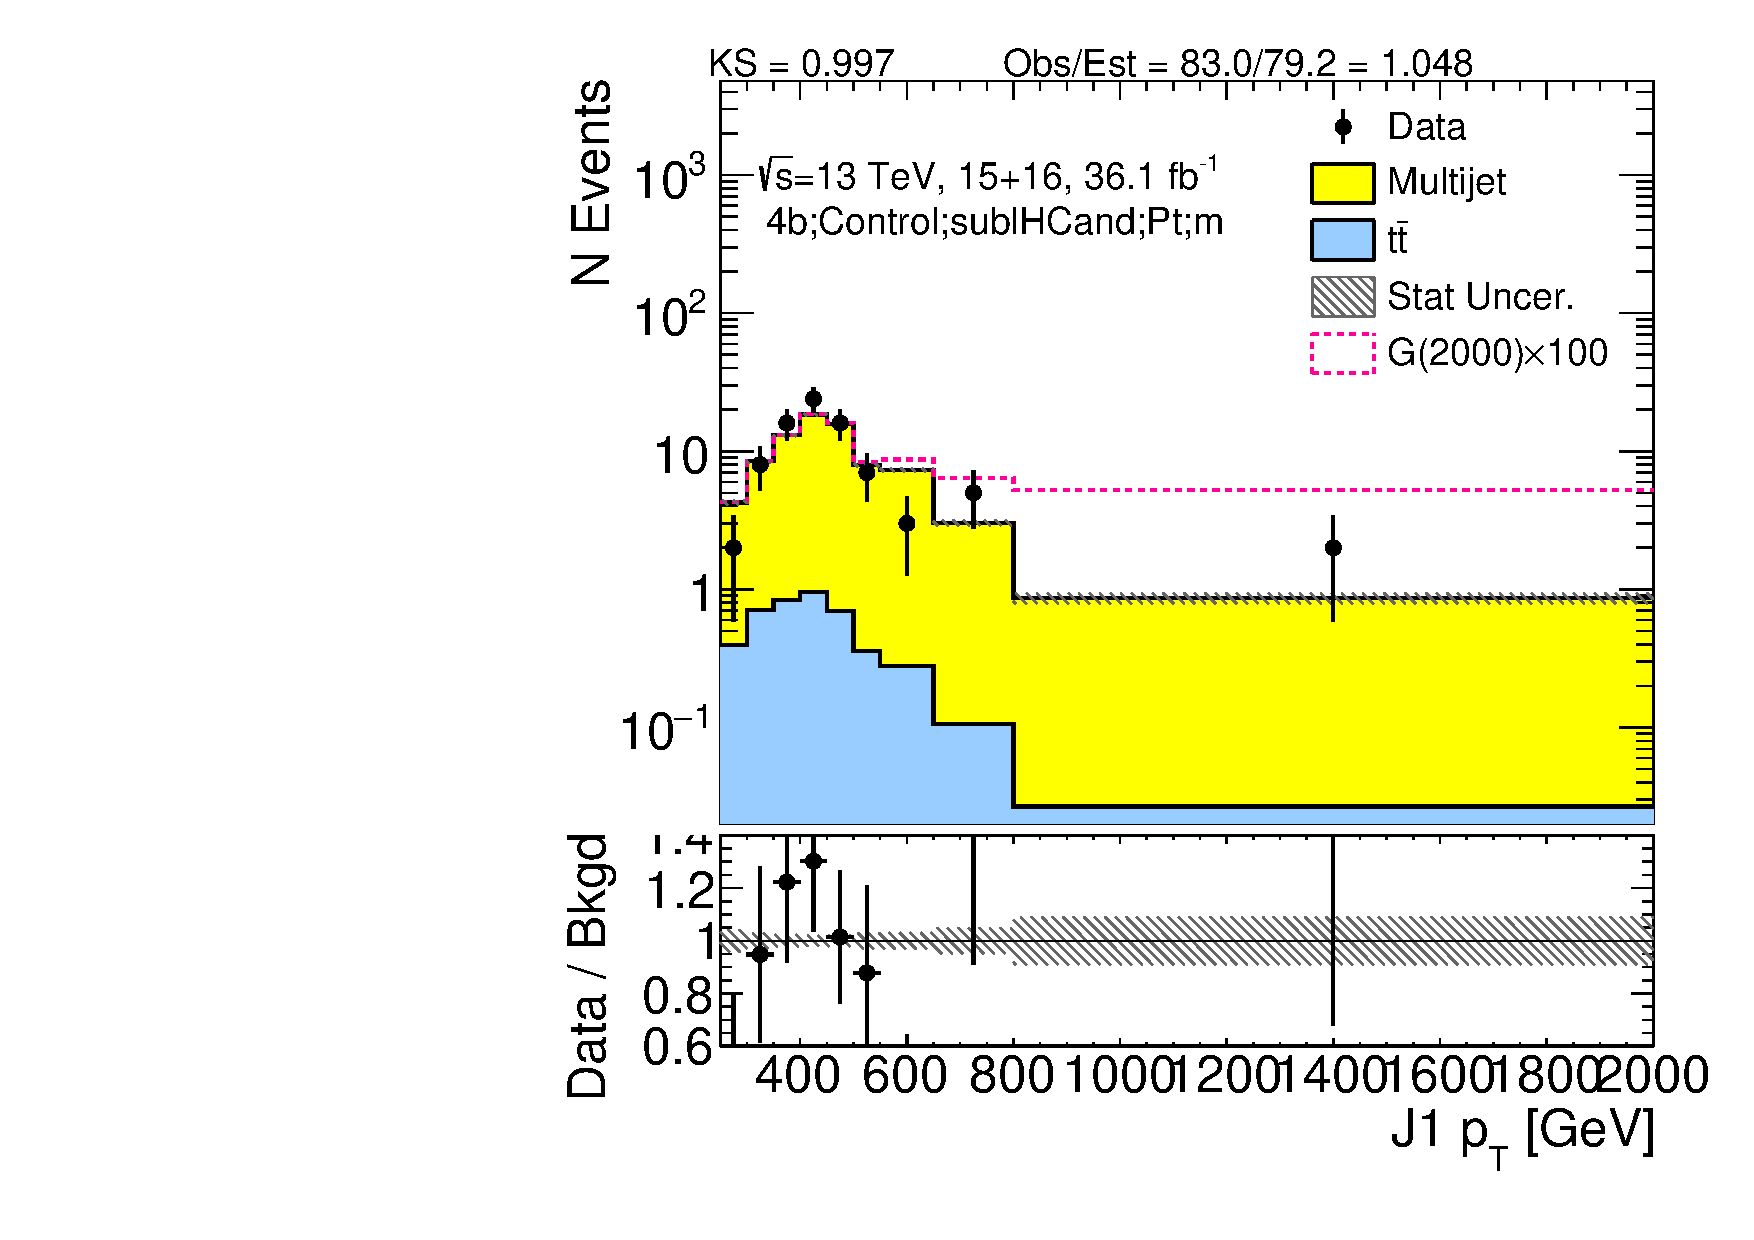
\includegraphics[width=0.33\textwidth, angle=270]{./figures/boosted/Control/Moriond_FourTag_Control_sublHCand_Pt_m_1.pdf}
0.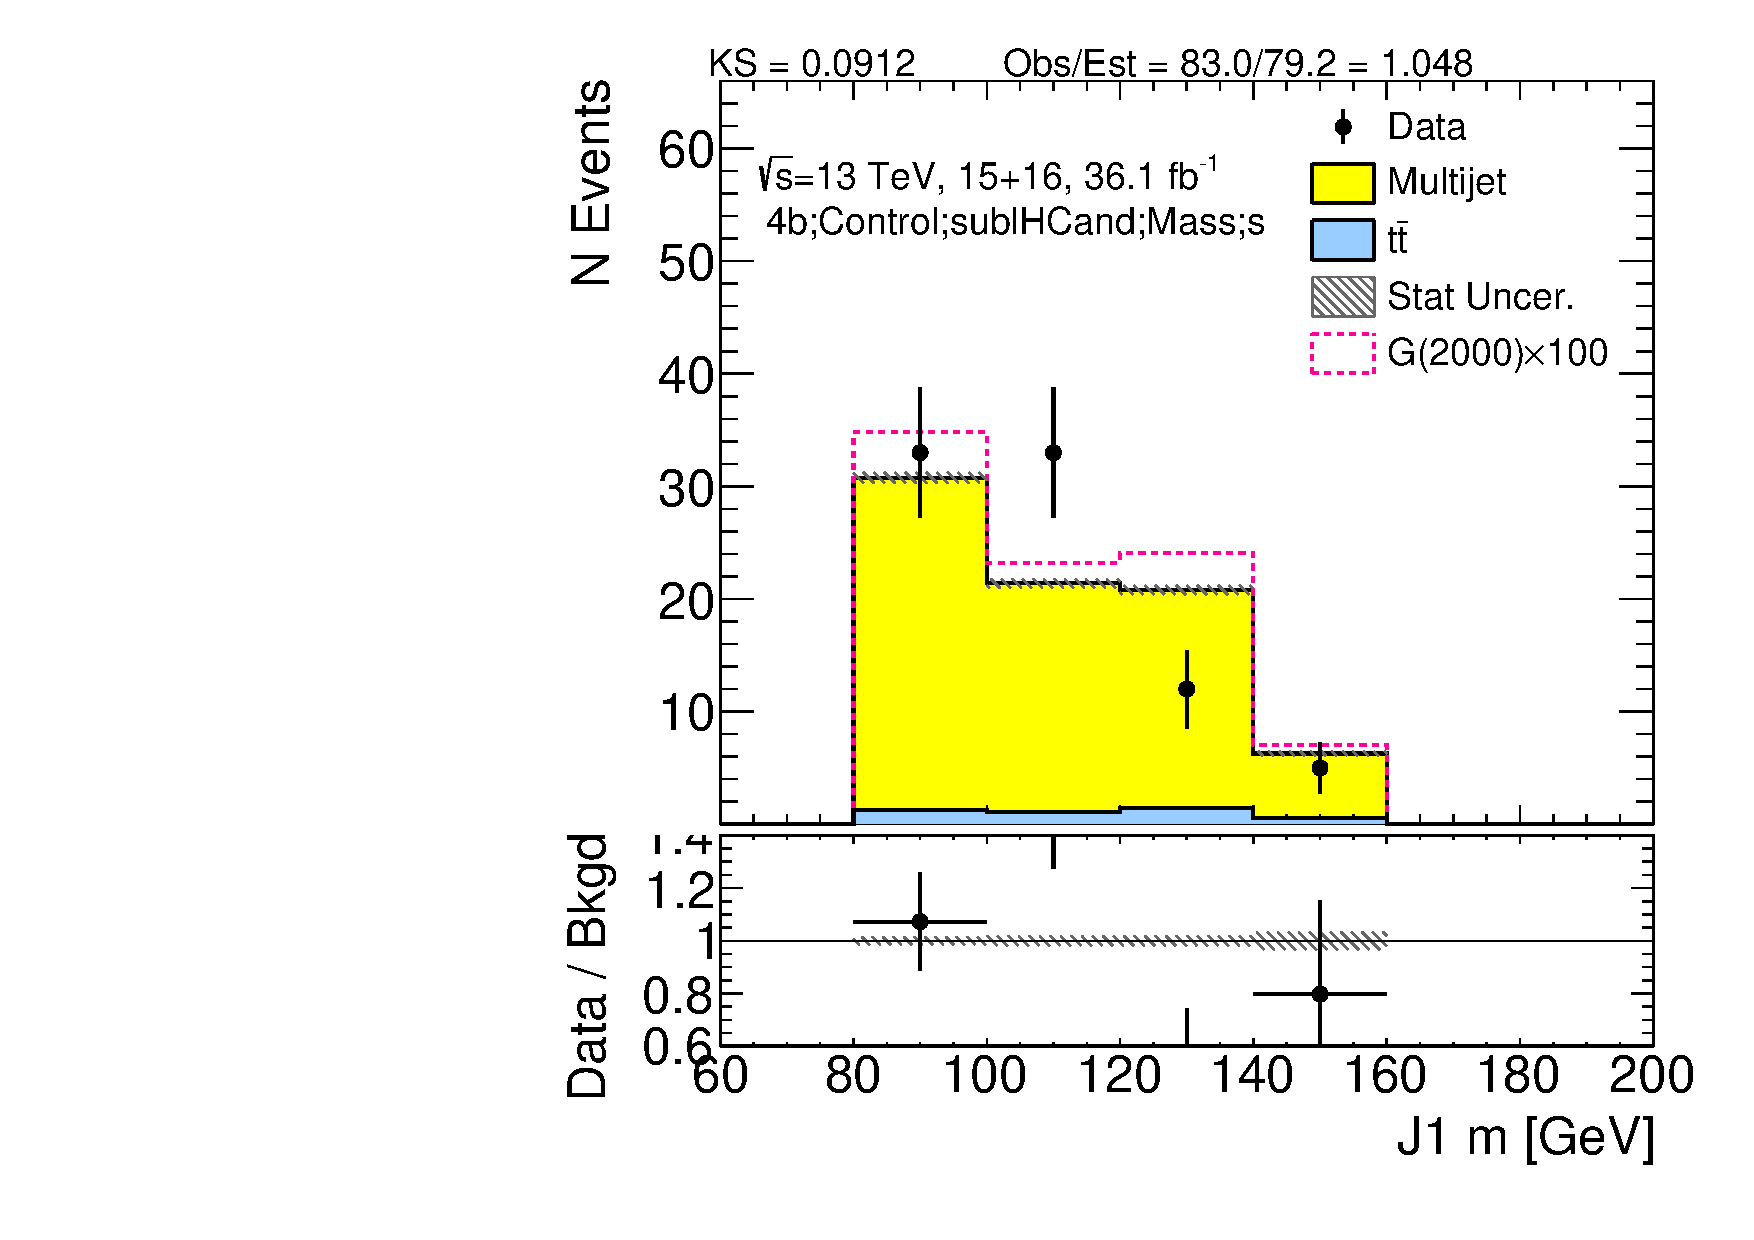
\includegraphics[width=0.33\textwidth, angle=270]{./figures/boosted/Control/Moriond_FourTag_Control_sublHCand_Mass_s.pdf}\\
0.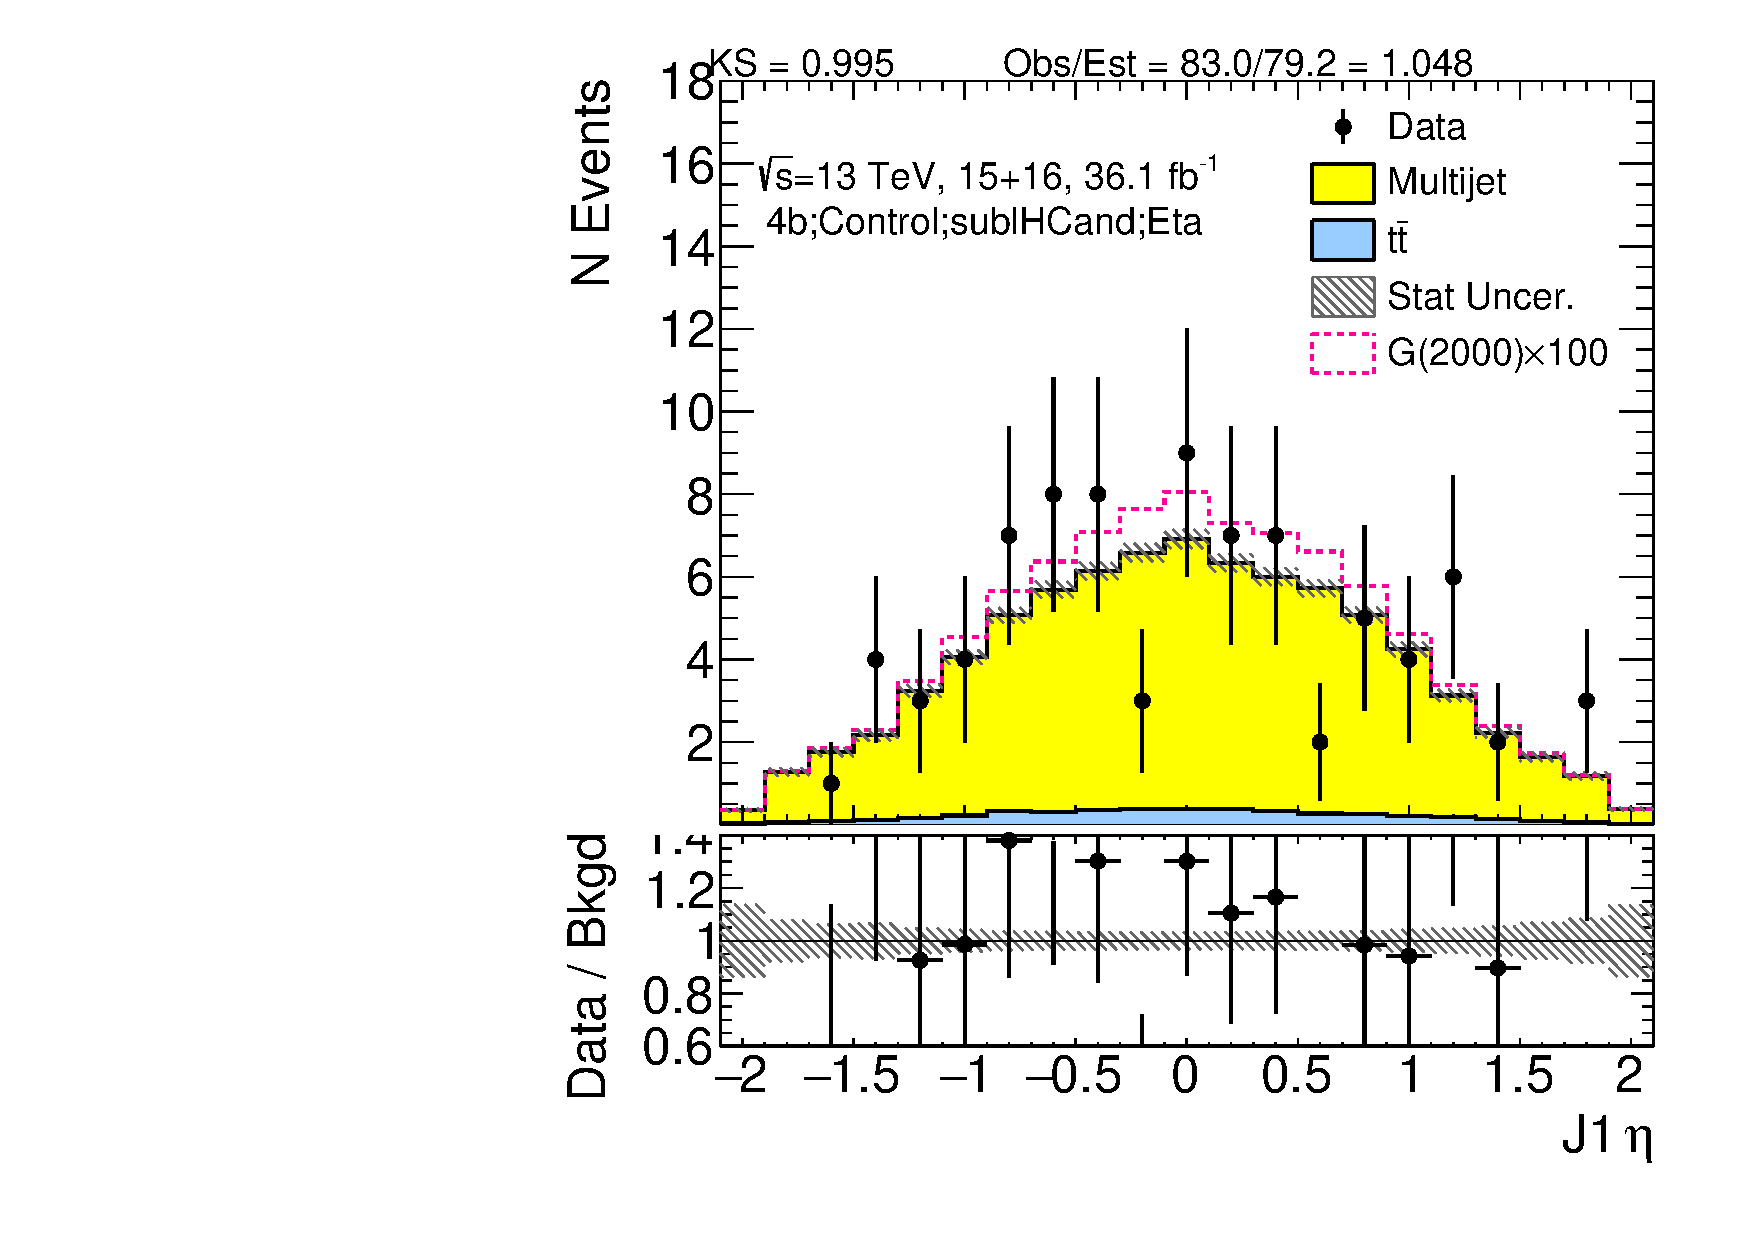
\includegraphics[width=0.33\textwidth, angle=270]{./figures/boosted/Control/Moriond_FourTag_Control_sublHCand_Eta.pdf}
0.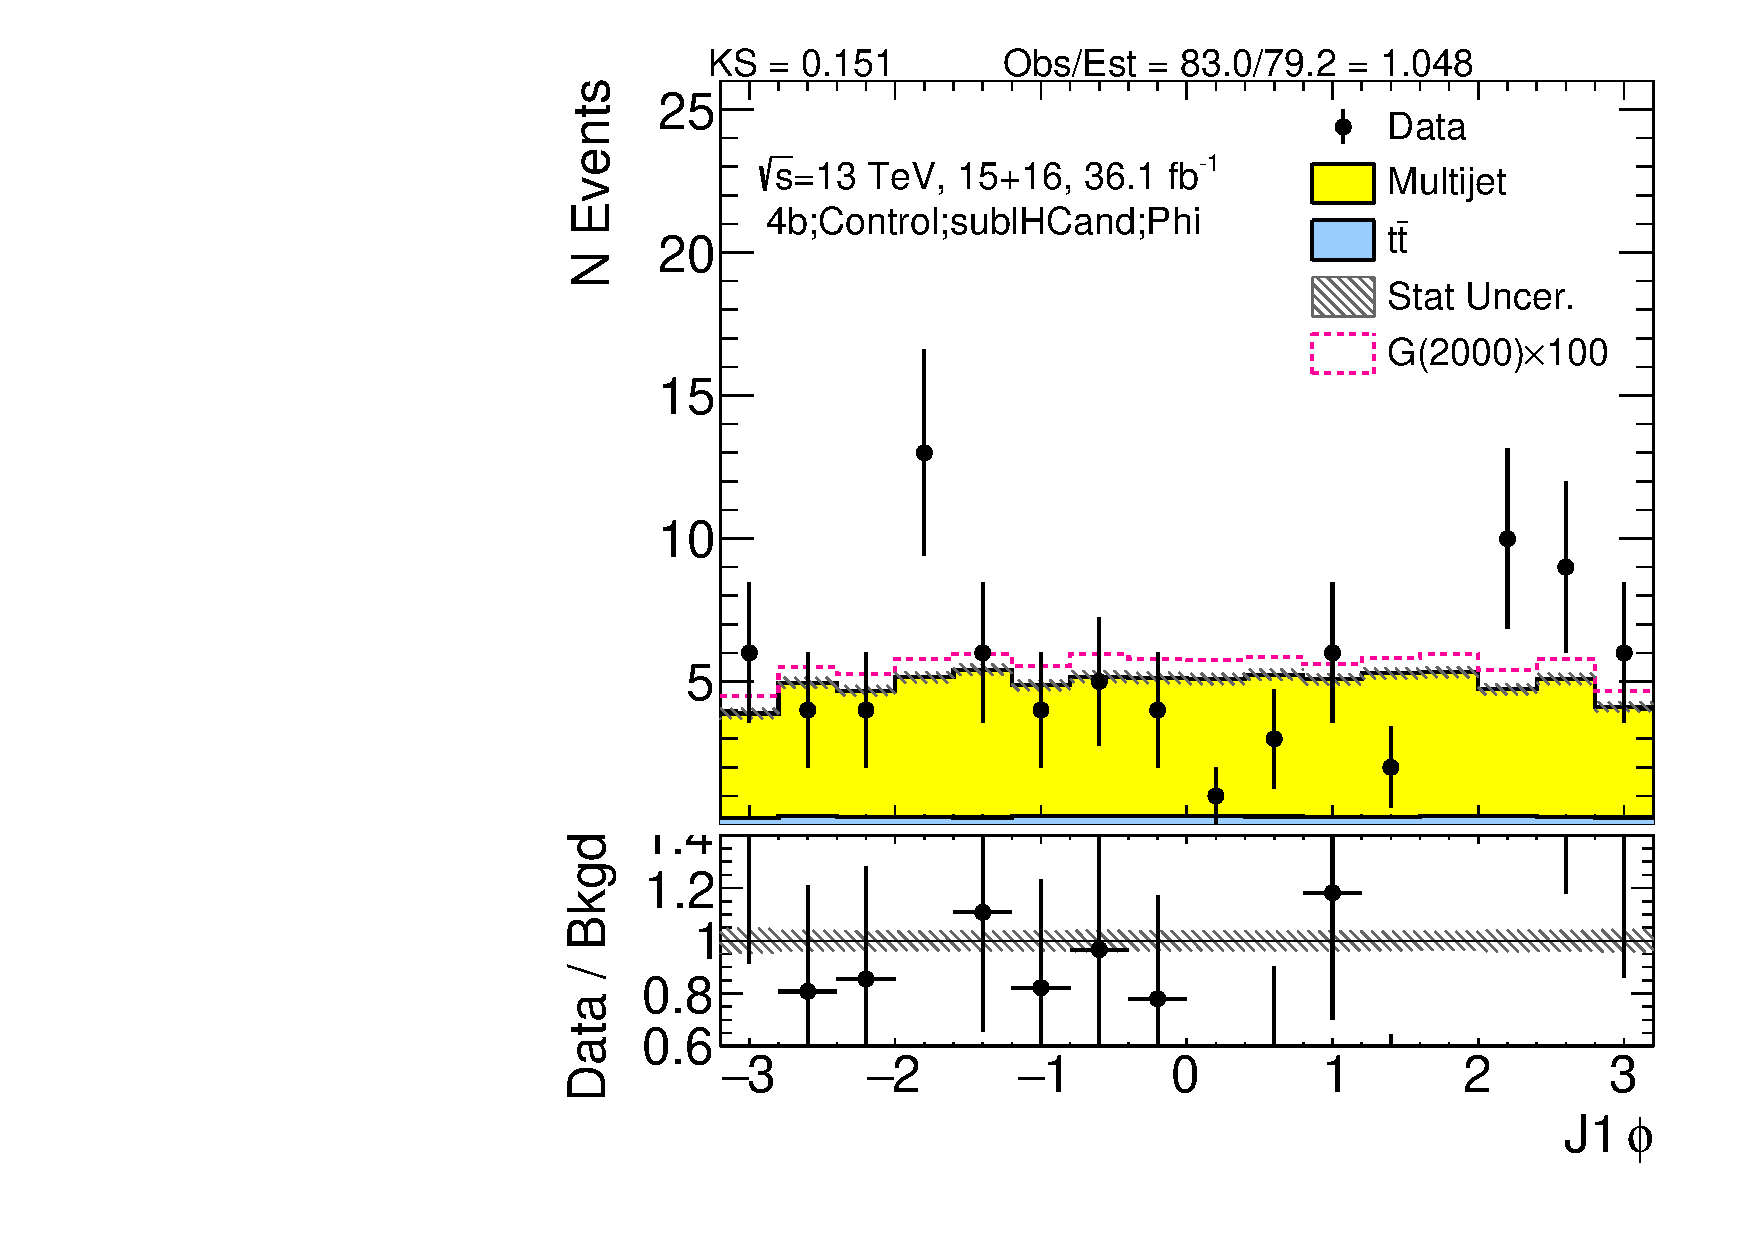
\includegraphics[width=0.33\textwidth, angle=270]{./figures/boosted/Control/Moriond_FourTag_Control_sublHCand_Phi.pdf}
  \caption{Kinematics of the sub-lead large-$R$ jet in data and prediction in the sideband region after requiring 4 $b$-tags. The normalization agrees by construction, and the shapes are a feature of the prediction.}
  \label{fig:boosted-4b-control-ak10-subl}
\end{center}
\end{figure*}

\begin{figure*}[htbp!]
\begin{center}
0.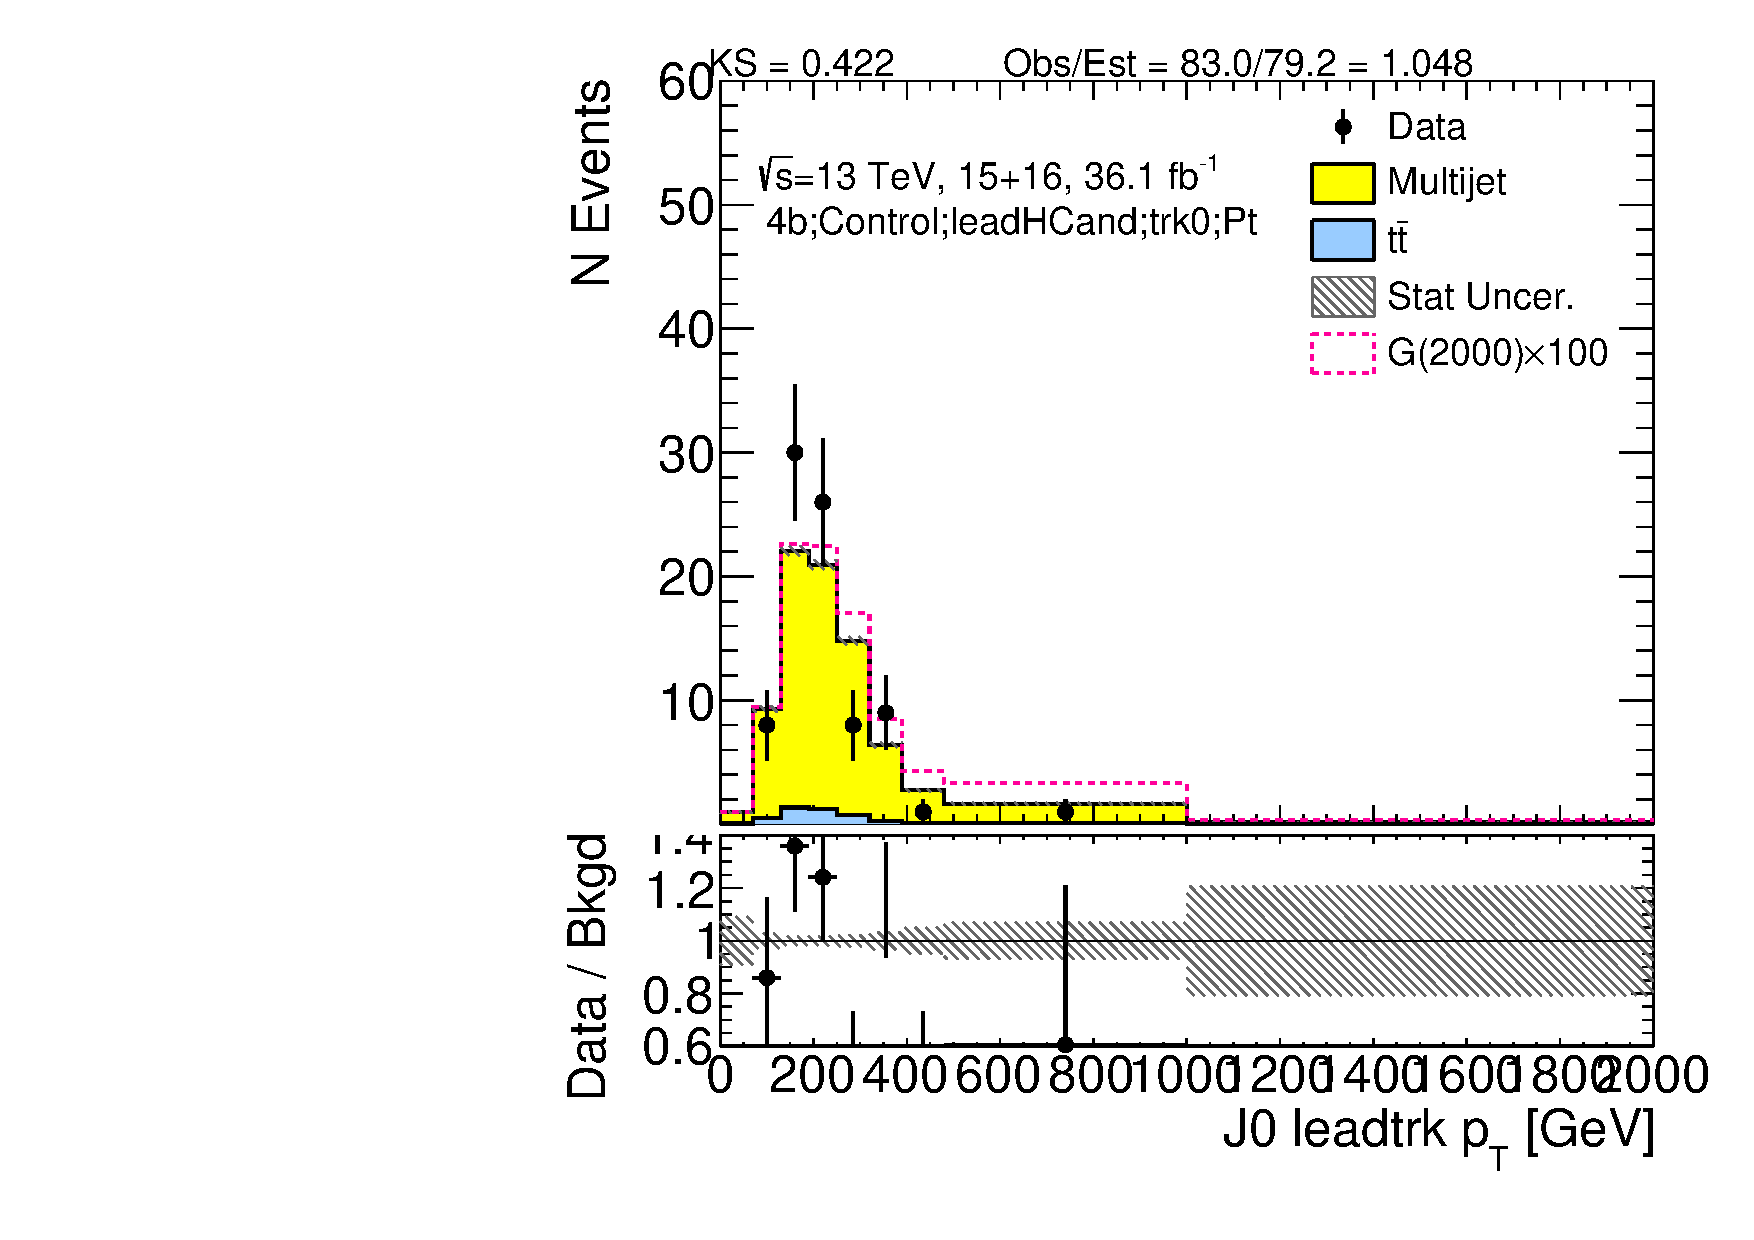
\includegraphics[width=0.33\textwidth, angle=270]{./figures/boosted/Control/Moriond_FourTag_Control_leadHCand_trk0_Pt.pdf}
0.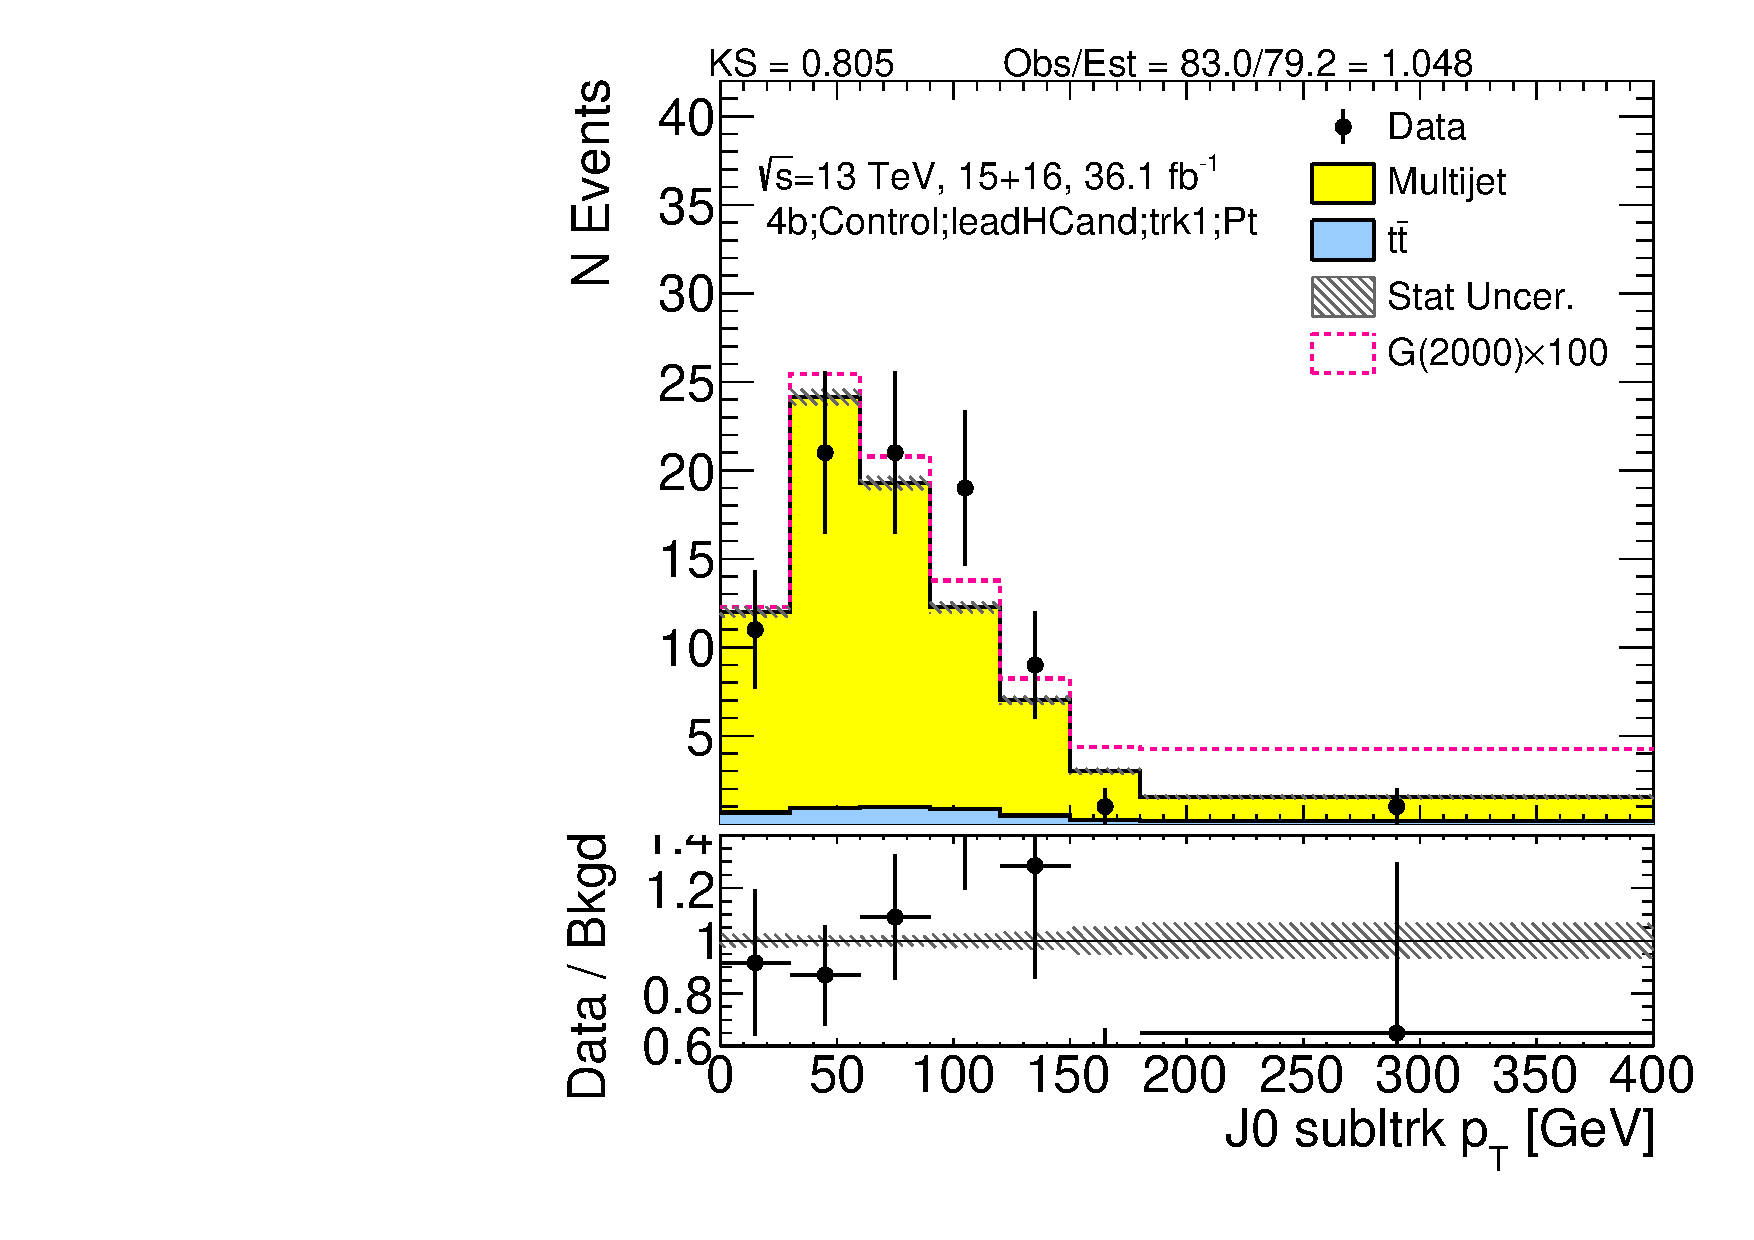
\includegraphics[width=0.33\textwidth, angle=270]{./figures/boosted/Control/Moriond_FourTag_Control_leadHCand_trk1_Pt.pdf}\\
0.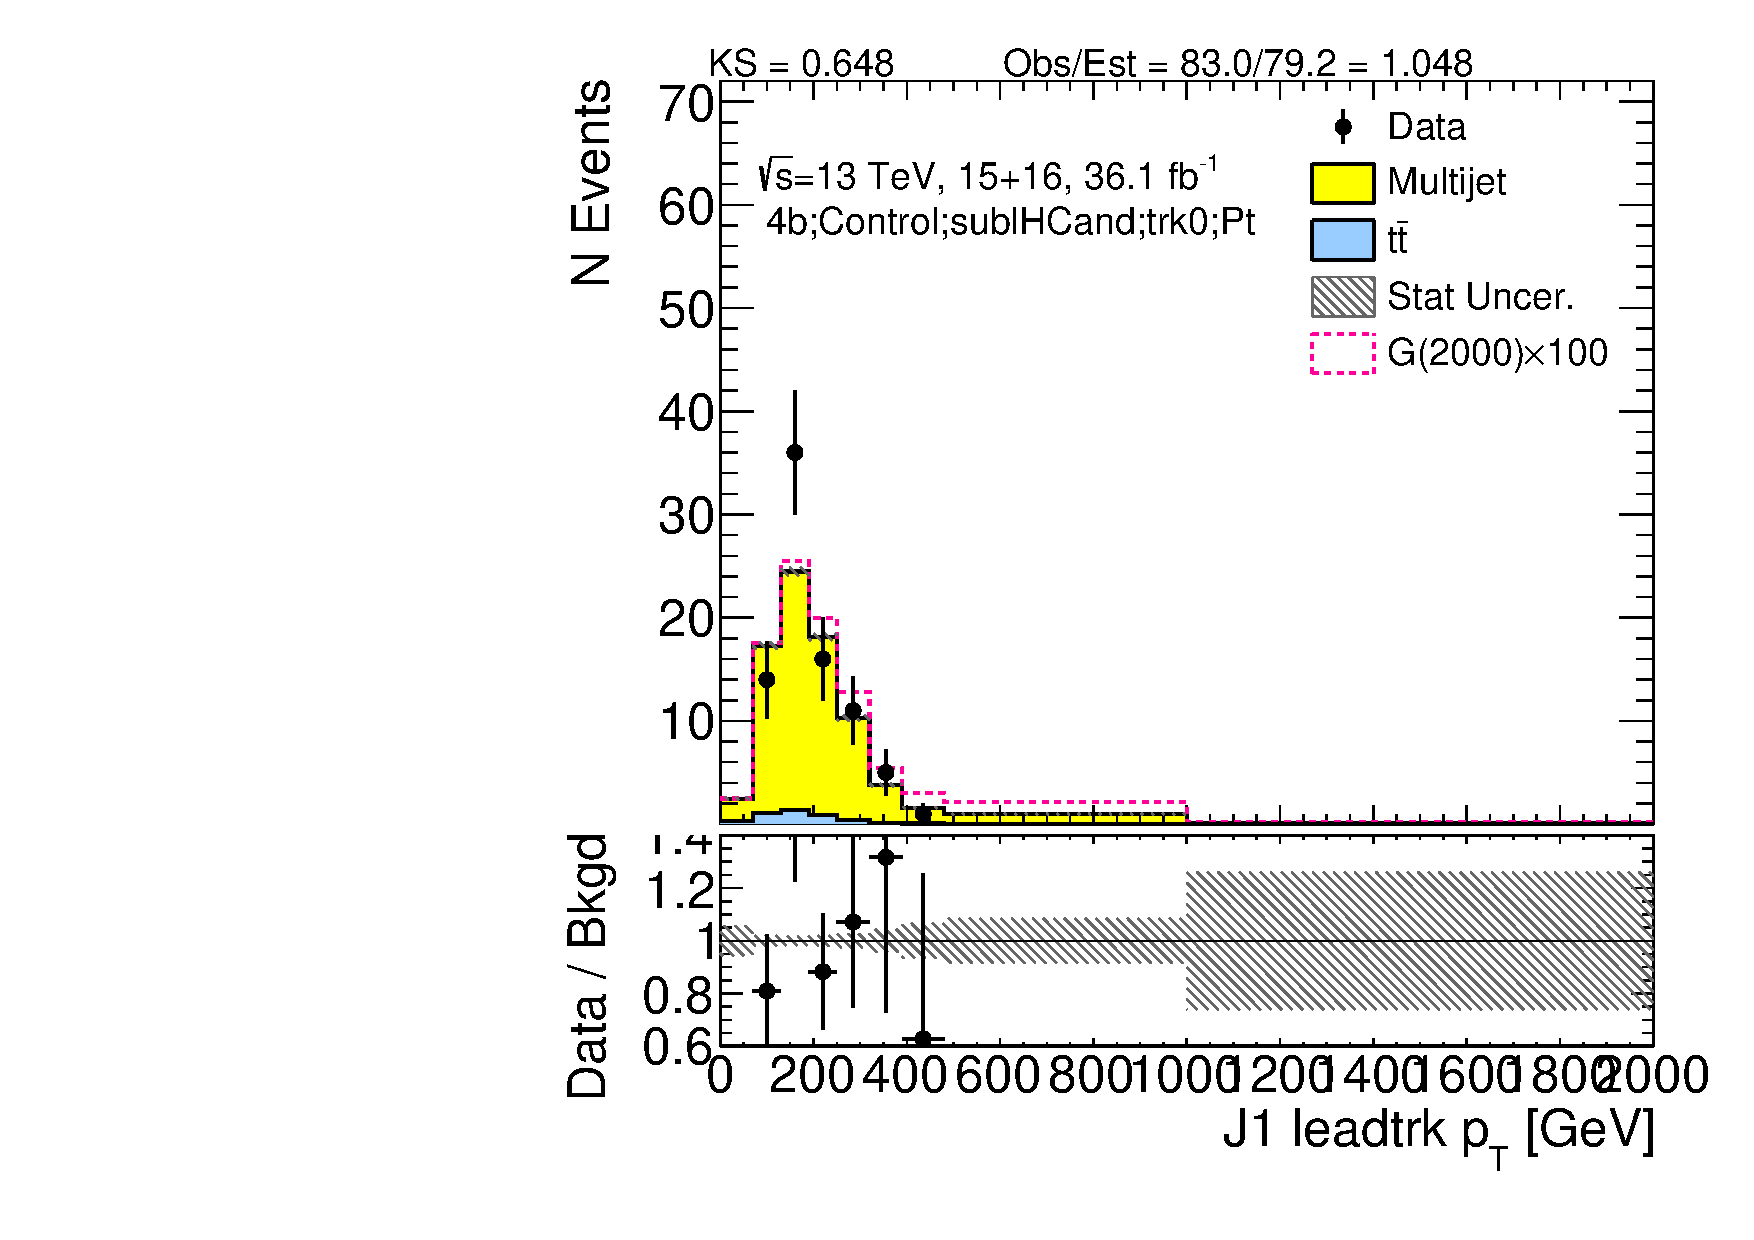
\includegraphics[width=0.33\textwidth, angle=270]{./figures/boosted/Control/Moriond_FourTag_Control_sublHCand_trk0_Pt.pdf}
0.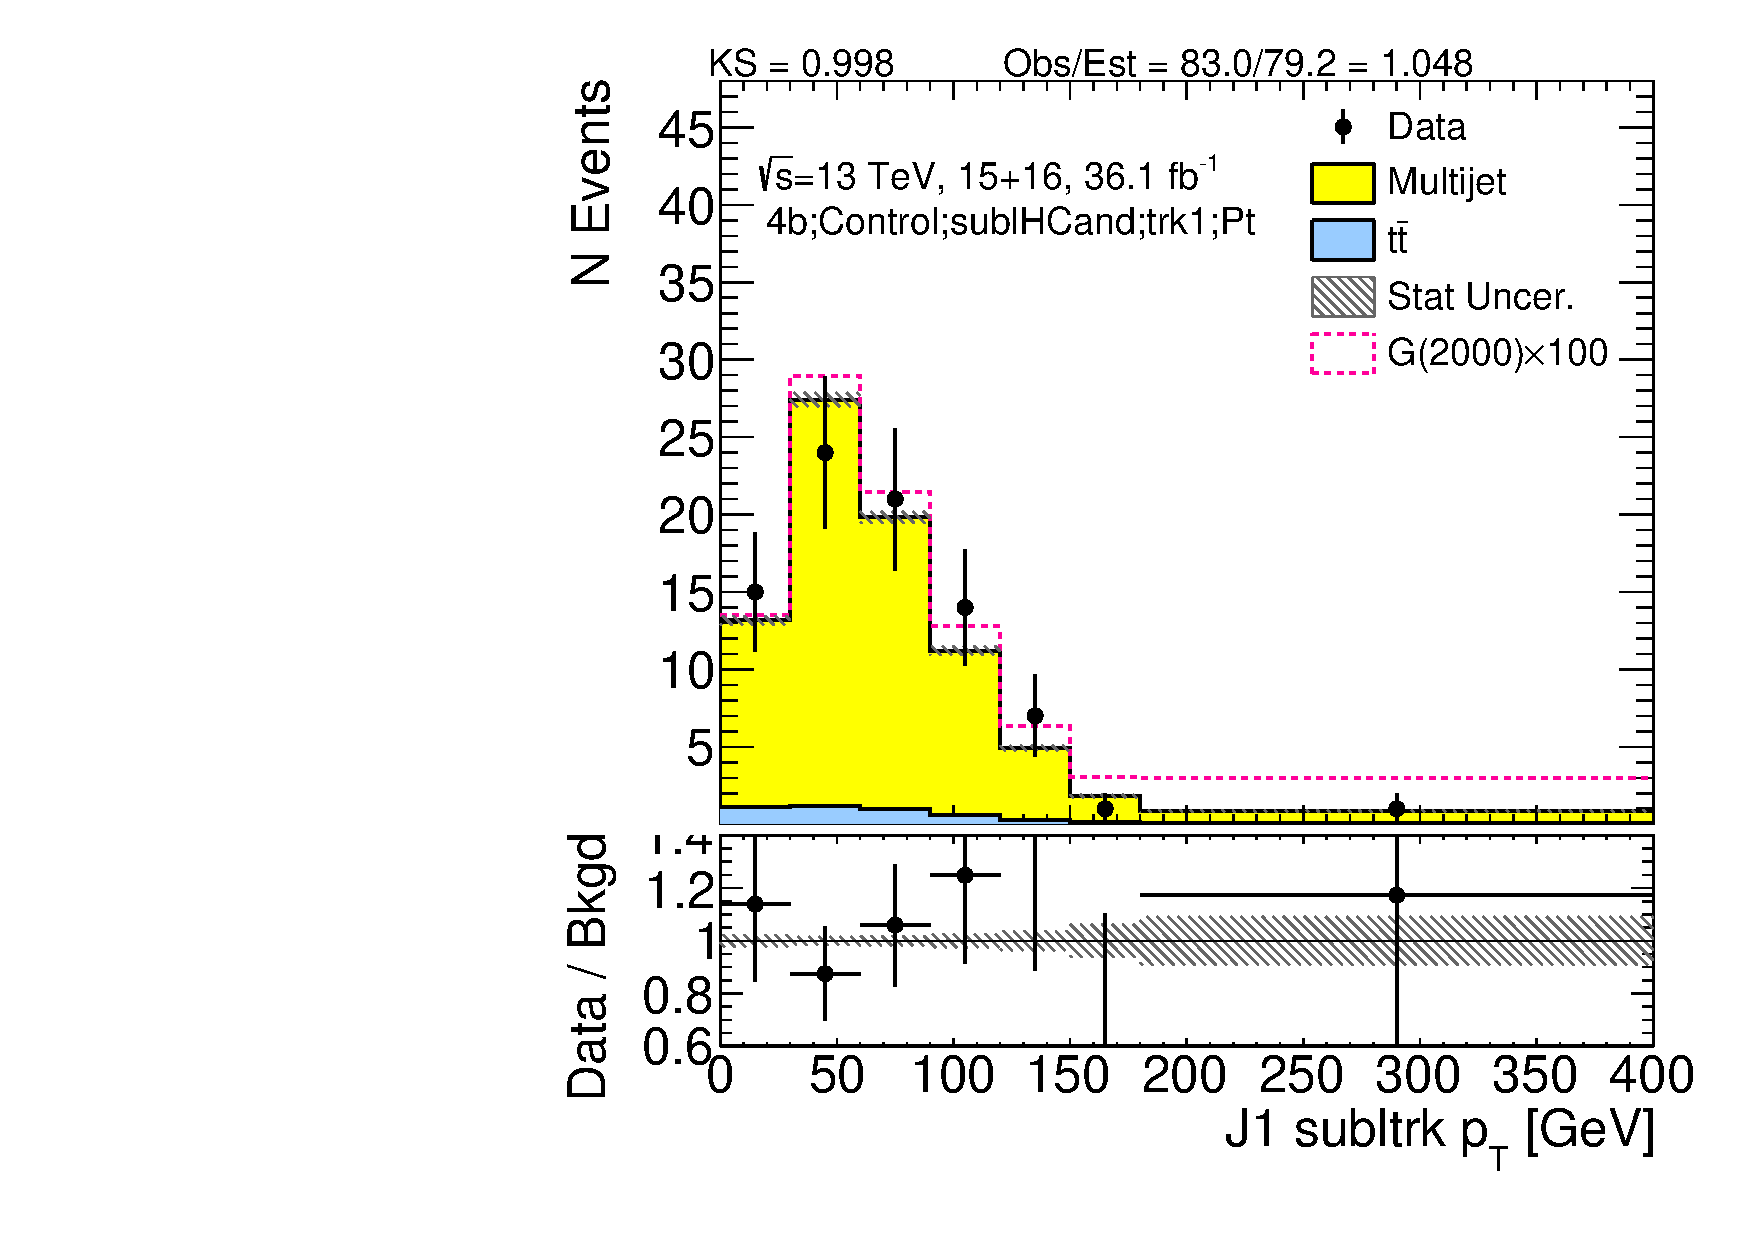
\includegraphics[width=0.33\textwidth, angle=270]{./figures/boosted/Control/Moriond_FourTag_Control_sublHCand_trk1_Pt.pdf}\\
0.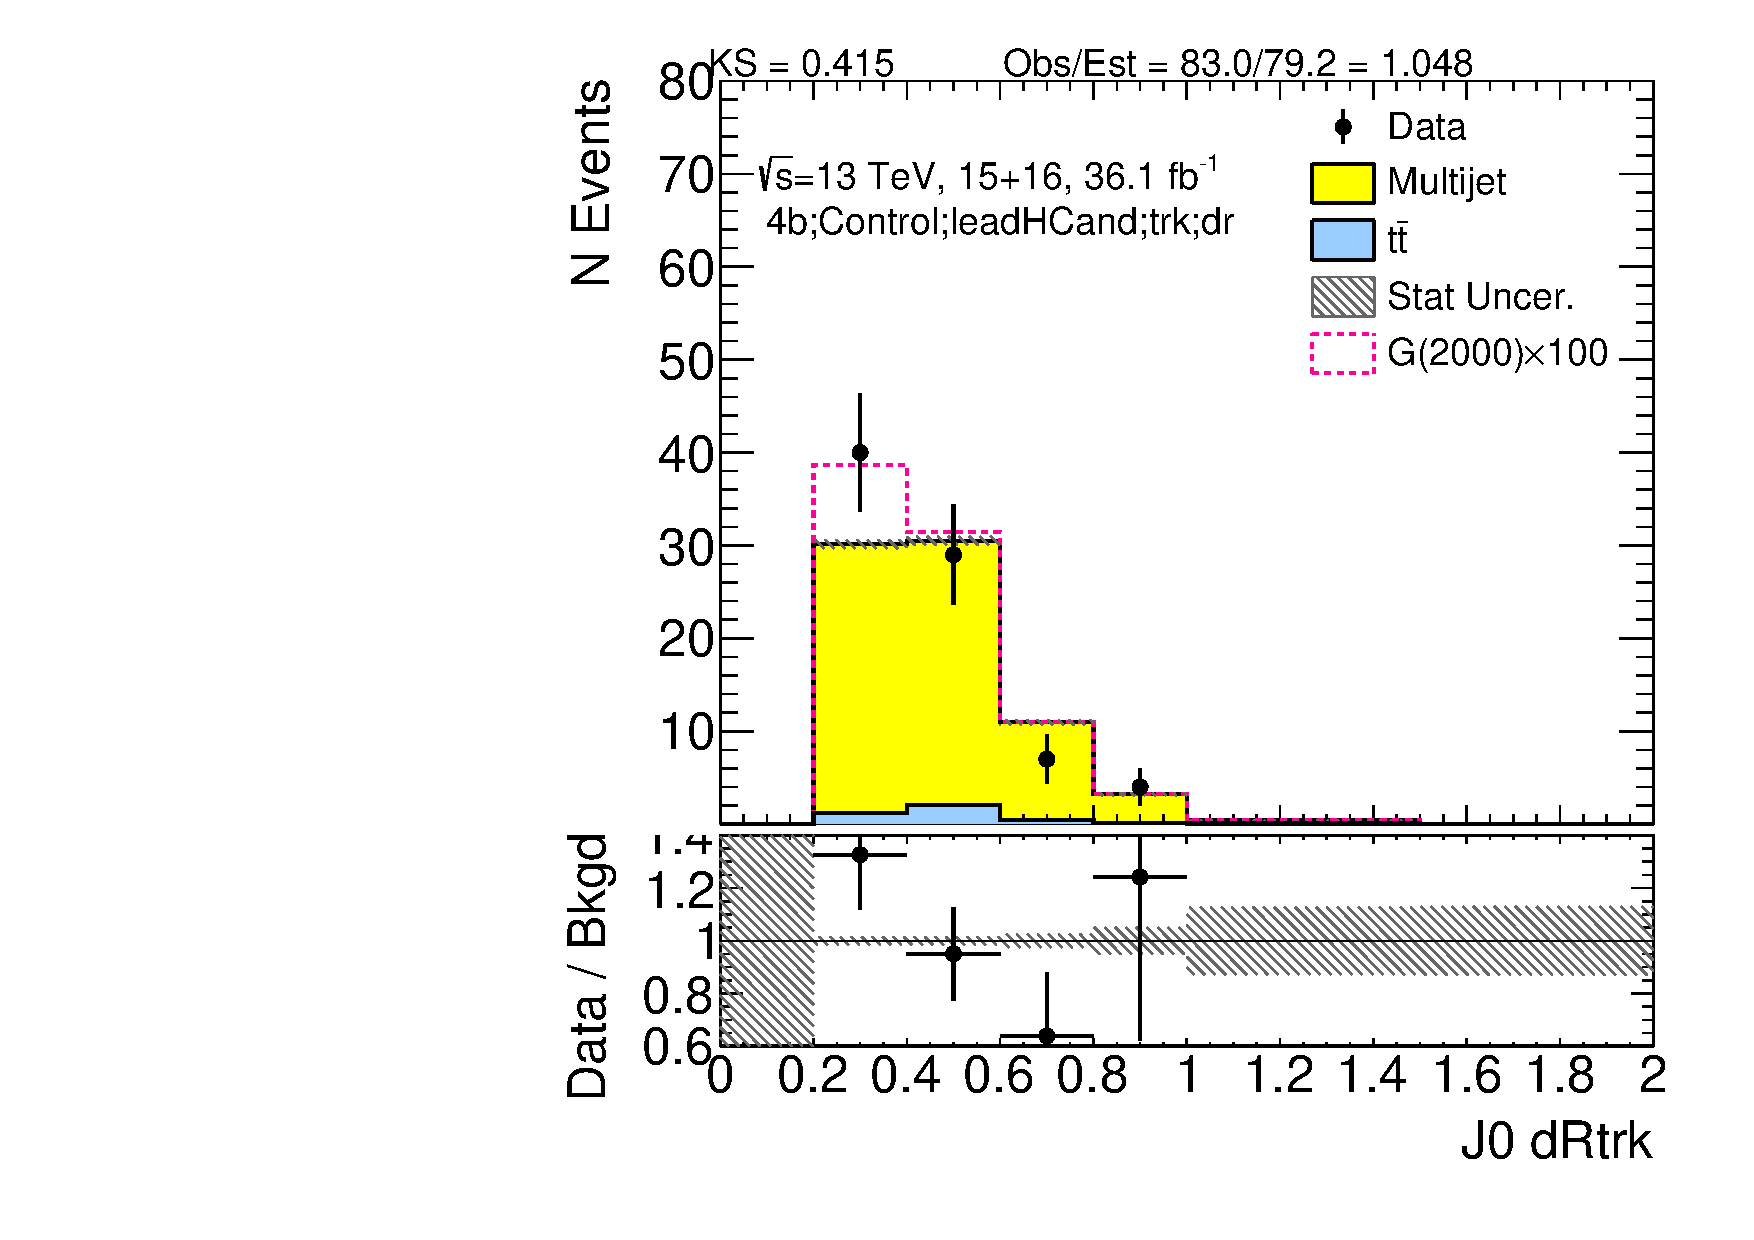
\includegraphics[width=0.33\textwidth, angle=270]{./figures/boosted/Control/Moriond_FourTag_Control_leadHCand_trk_dr.pdf}
0.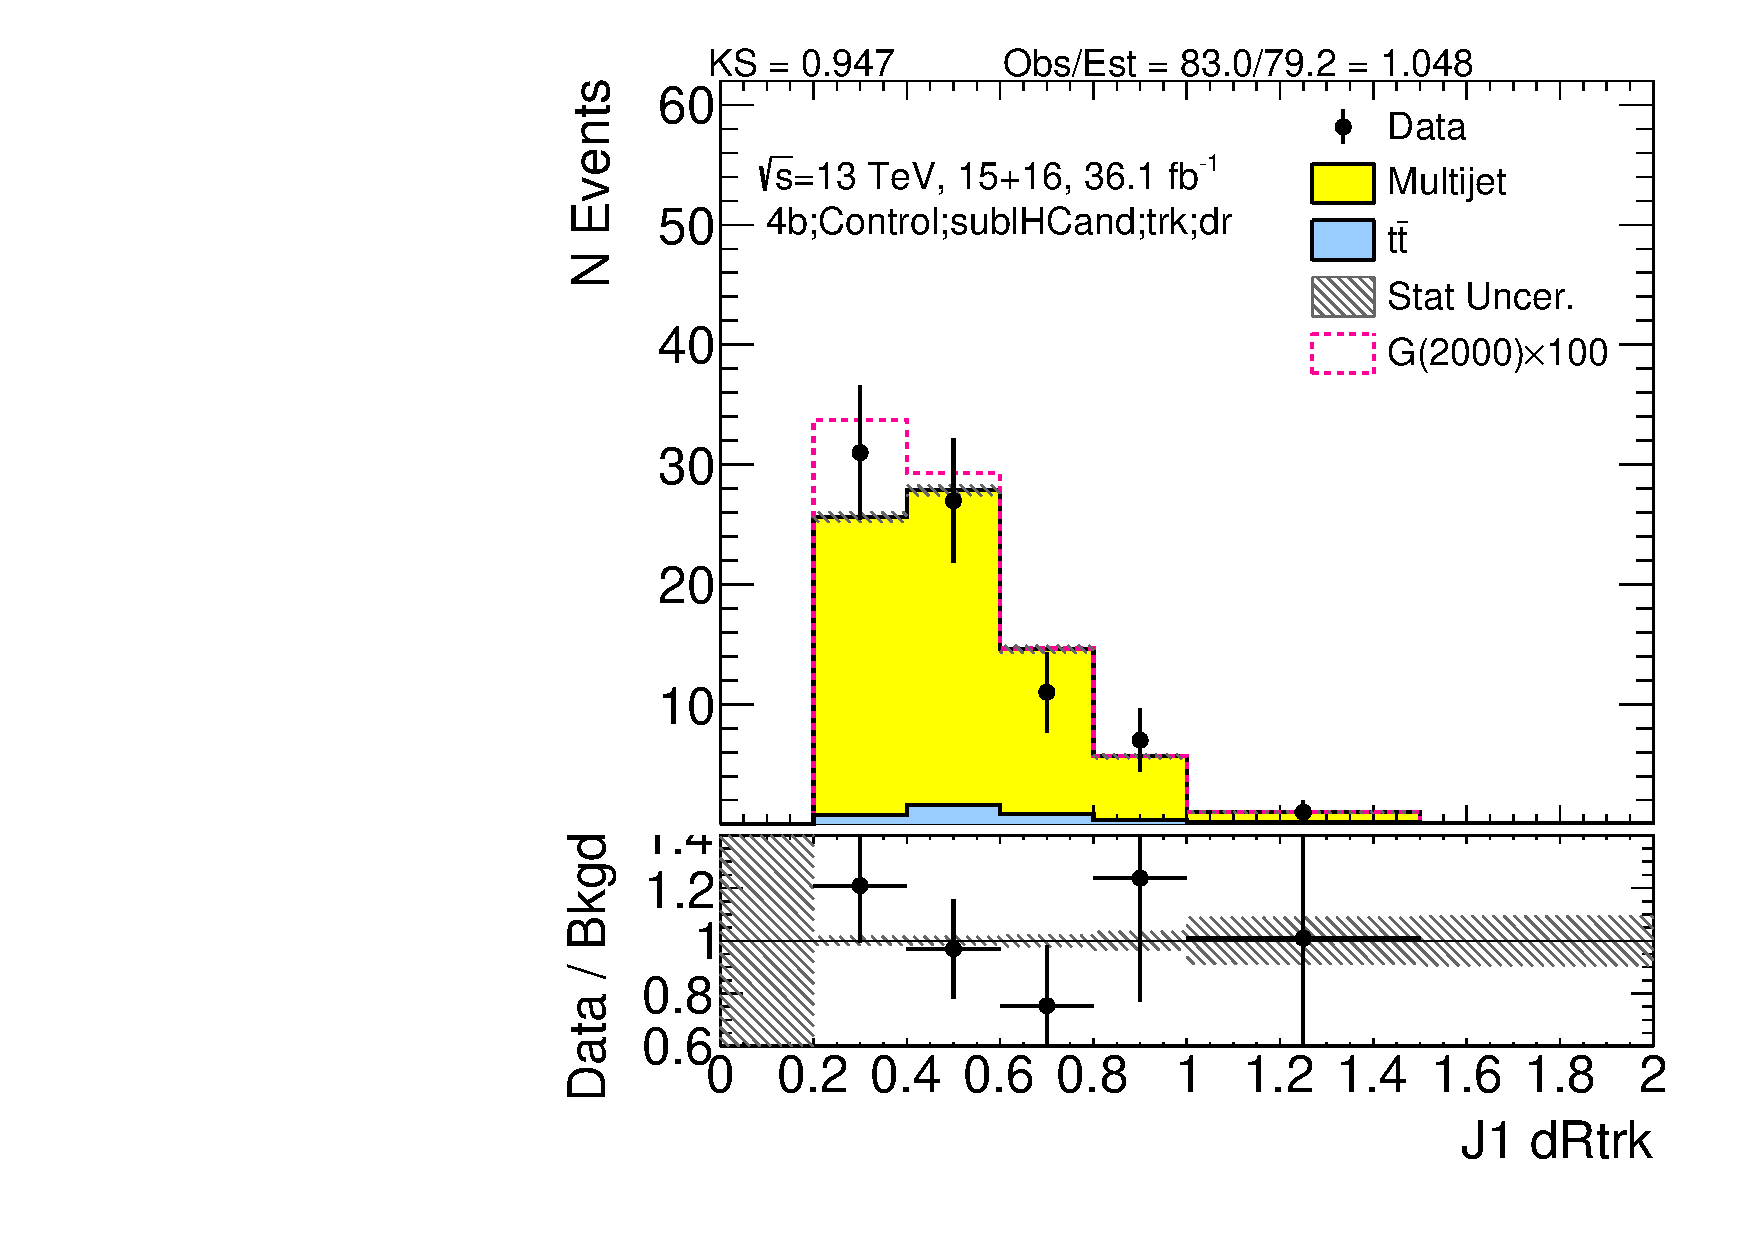
\includegraphics[width=0.33\textwidth, angle=270]{./figures/boosted/Control/Moriond_FourTag_Control_sublHCand_trk_dr.pdf}
  \caption{First two rows show the kinematics of the lead (left) and sub-lead (right) small-$R$ track jets associated to the lead (first-row) and sub-lead (second-row) large-$R$ jet in data and prediction in the sideband region after requiring 4 $b$-tags. Third row shows the $\Delta R$ between two leading small-$R$ track-jets associated to the leading (left) and sub-leading (right) large-$R$ jet. The normalization agrees by construction, and the shapes are a feature of the prediction. }
  \label{fig:boosted-4b-control-ak2}
\end{center}
\end{figure*}


\begin{figure*}[htbp!]
\begin{center}
0.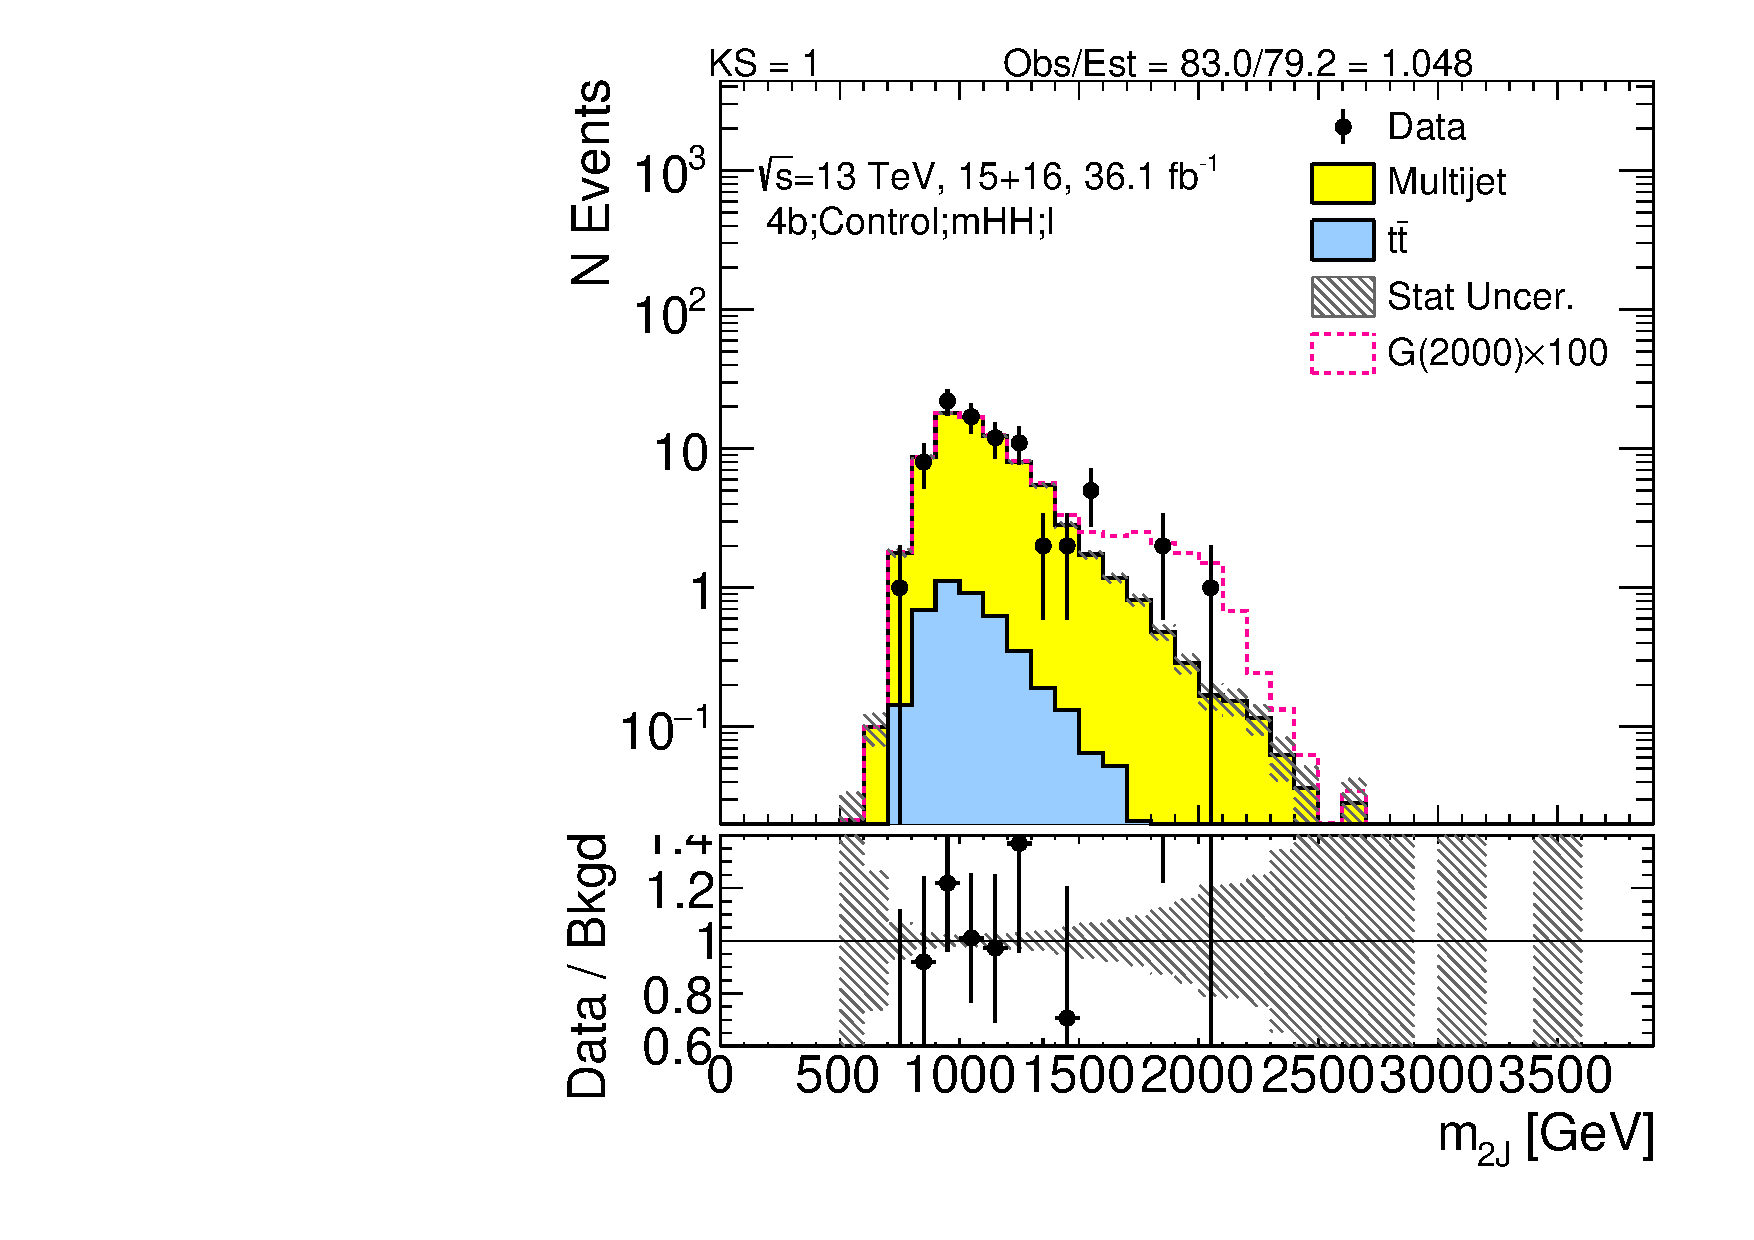
\includegraphics[width=0.33\textwidth, angle=270]{./figures/boosted/Control/Moriond_FourTag_Control_mHH_l_1.pdf}
0.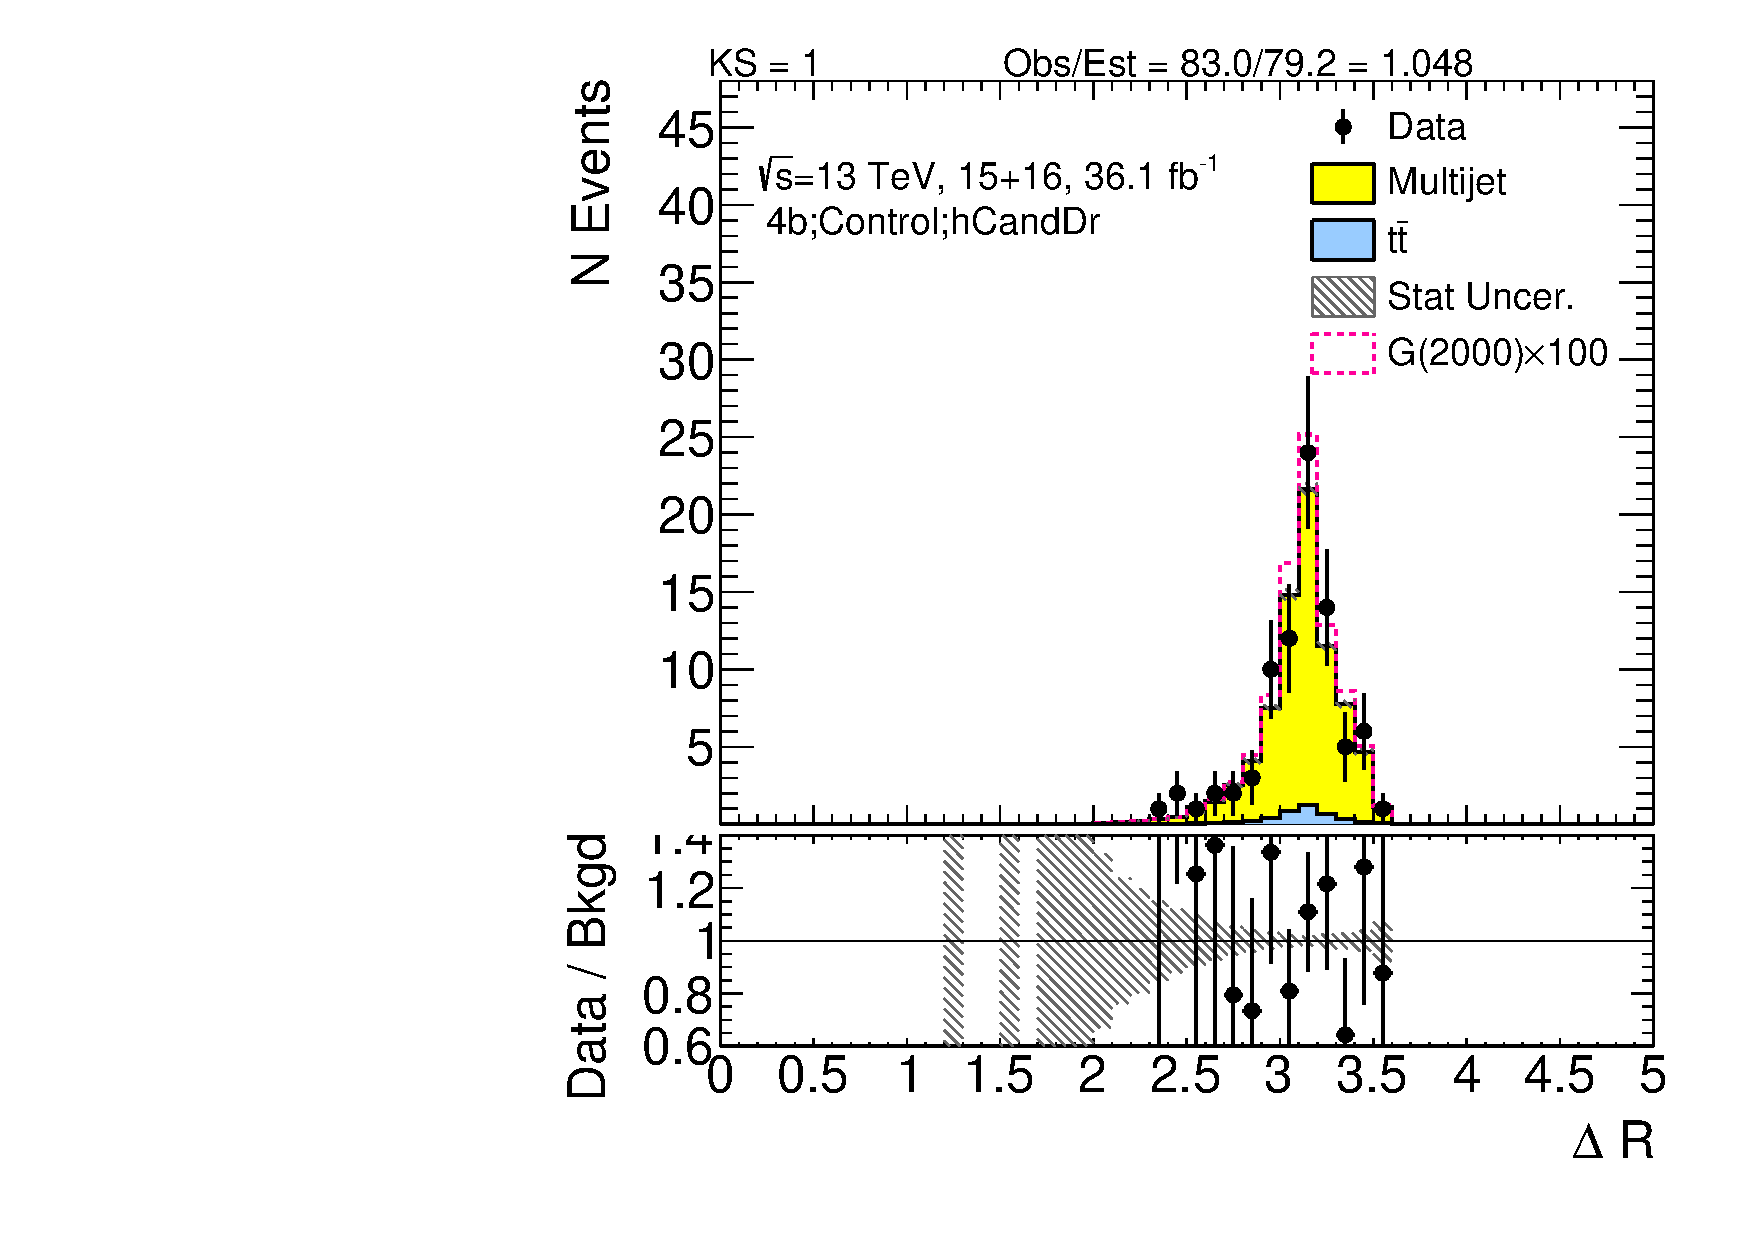
\includegraphics[width=0.33\textwidth, angle=270]{./figures/boosted/Control/Moriond_FourTag_Control_hCandDr.pdf}\\
0.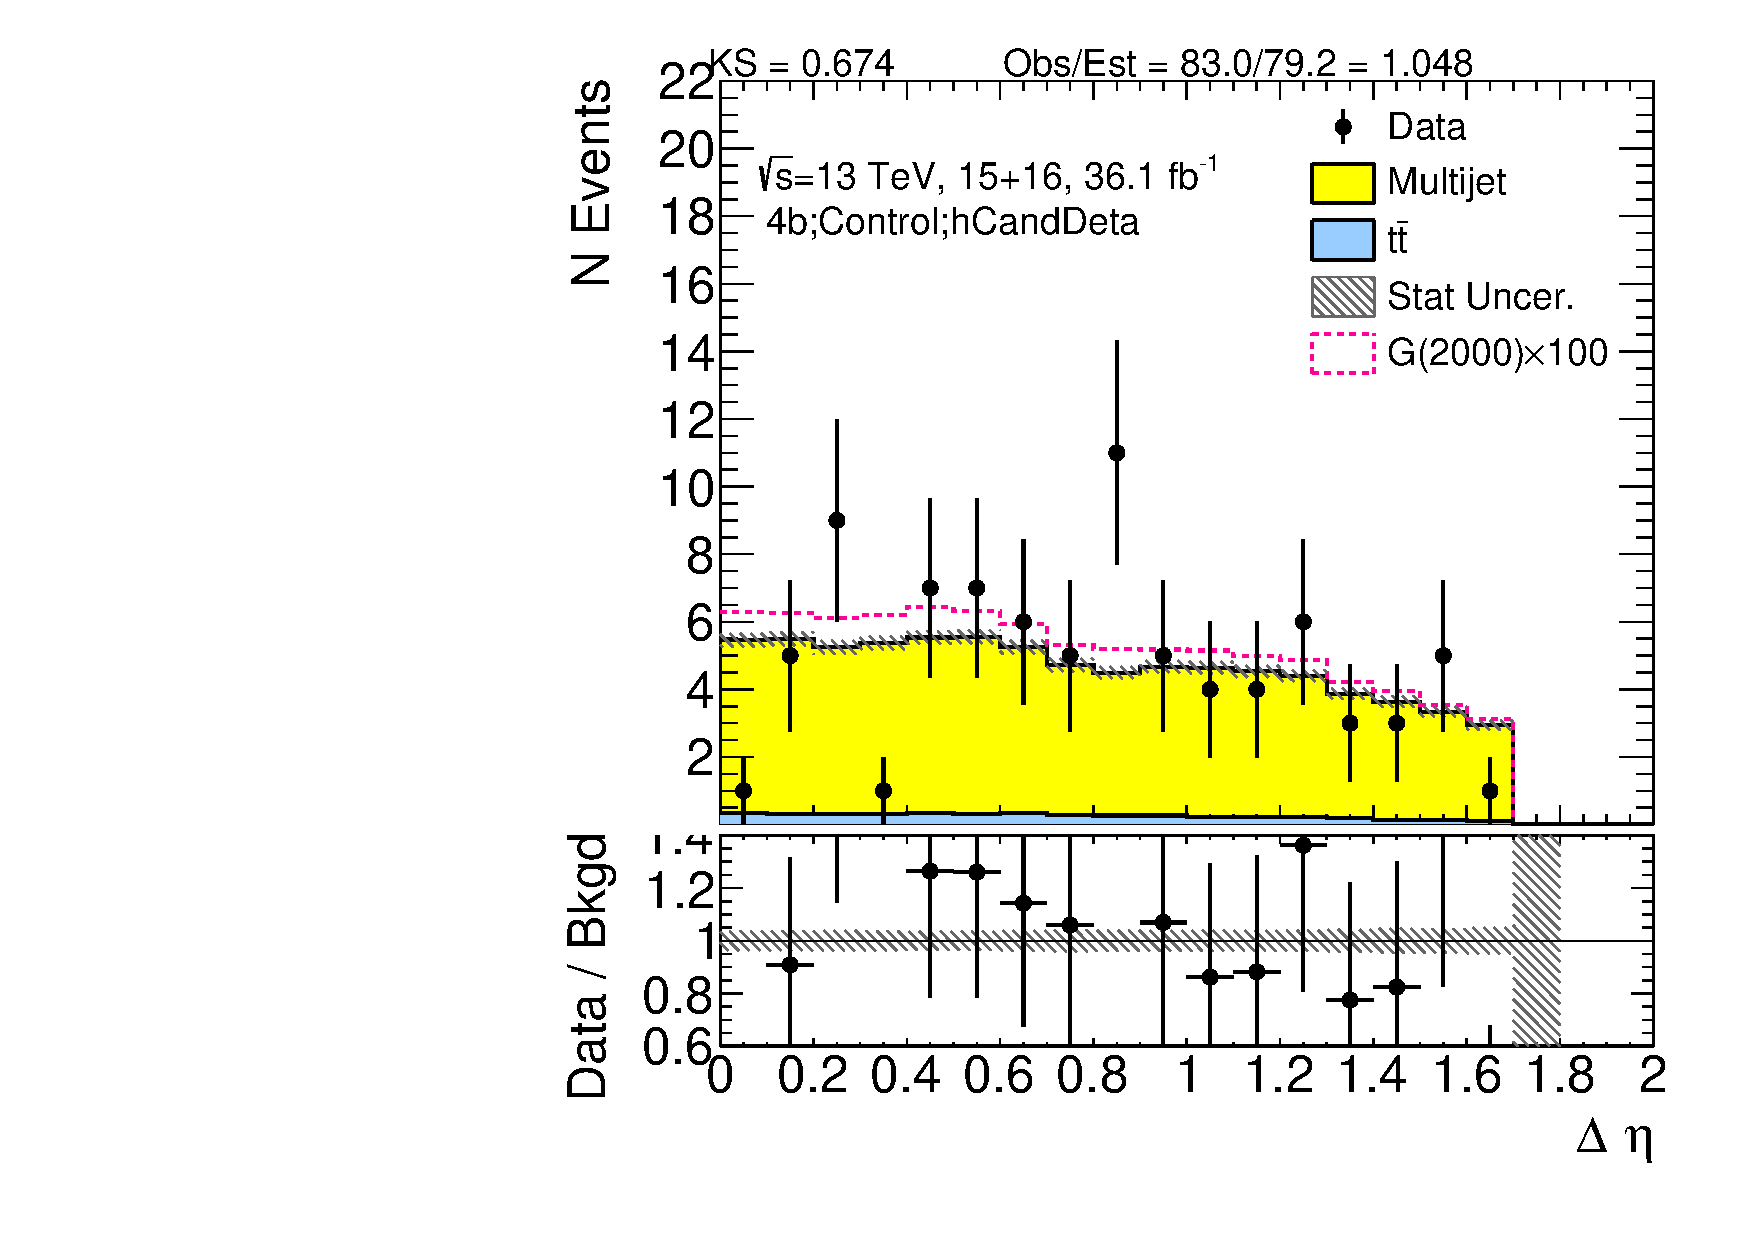
\includegraphics[width=0.33\textwidth, angle=270]{./figures/boosted/Control/Moriond_FourTag_Control_hCandDeta.pdf}
0.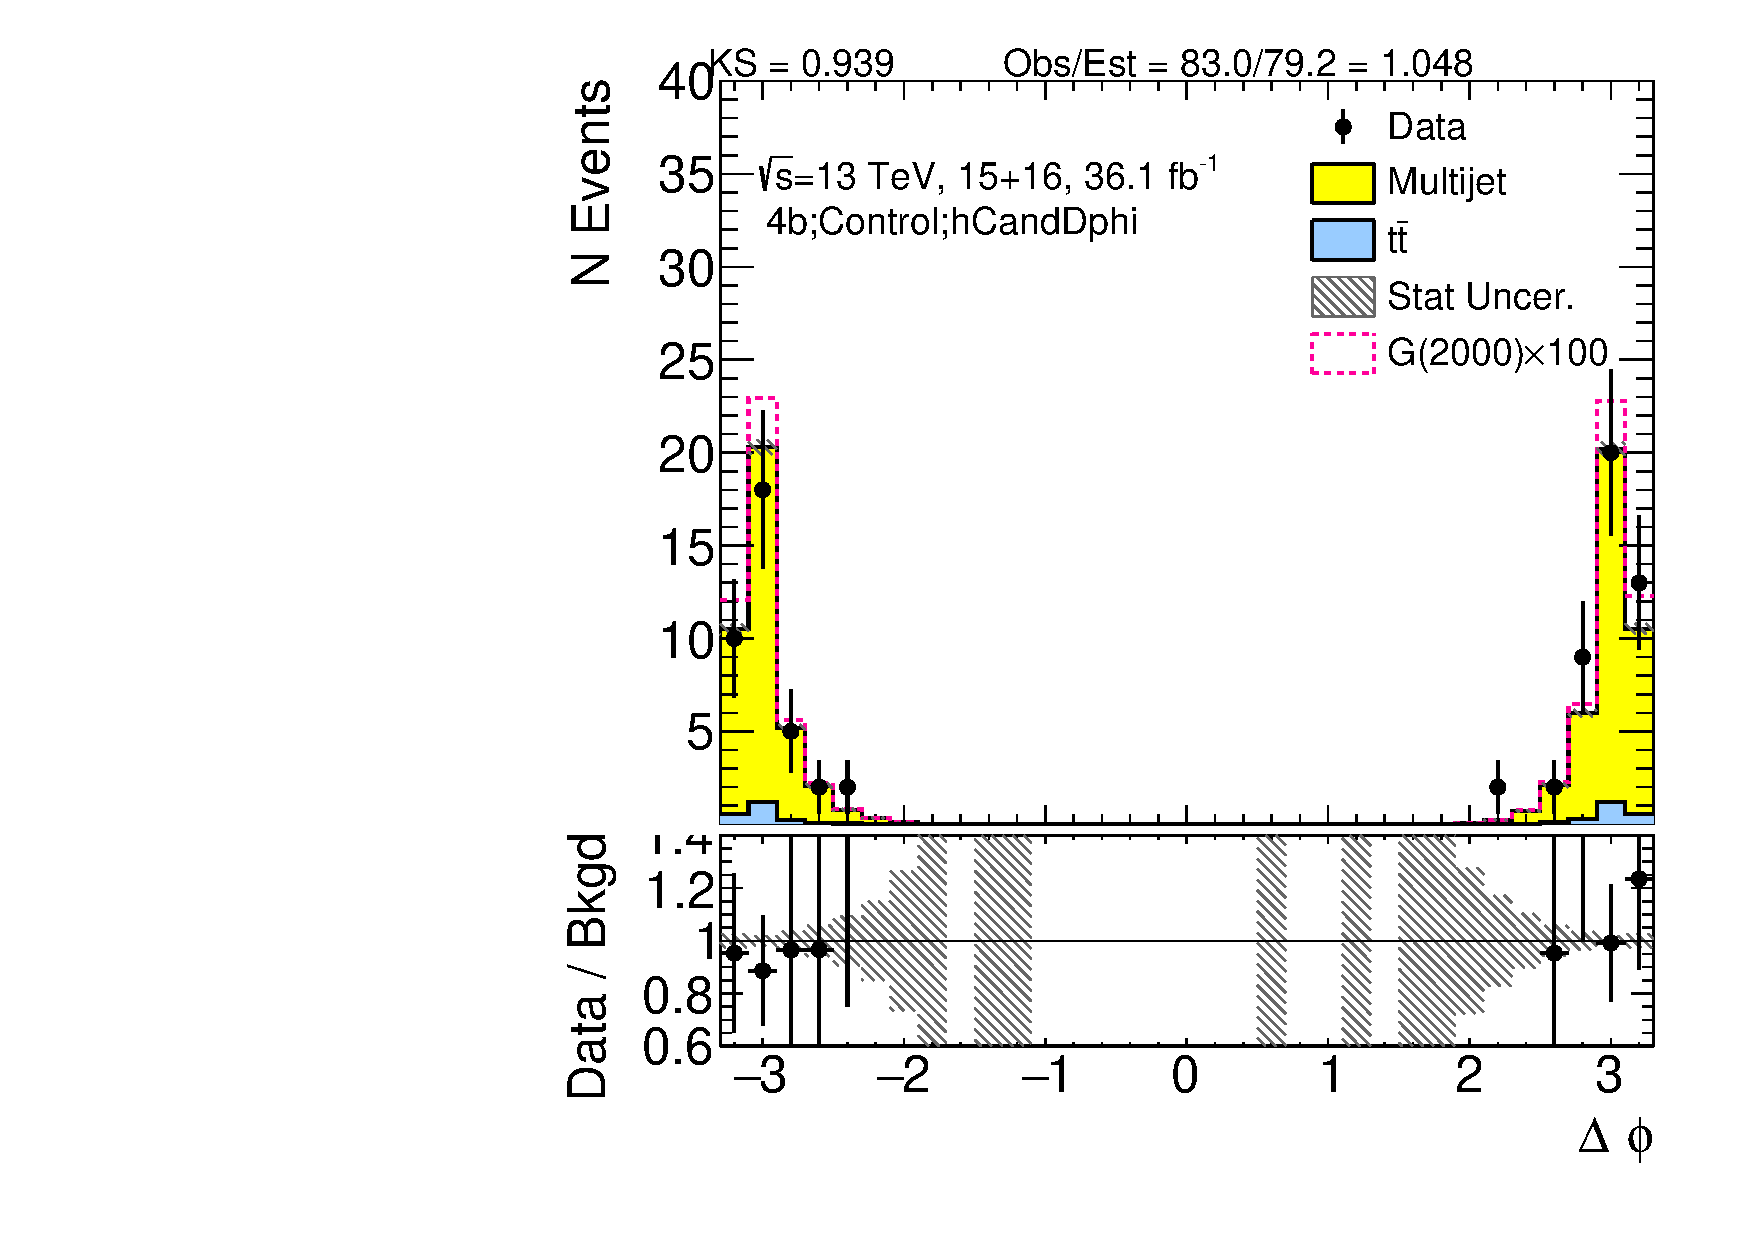
\includegraphics[width=0.33\textwidth, angle=270]{./figures/boosted/Control/Moriond_FourTag_Control_hCandDphi.pdf}
  \caption{Kinematics of the large-$R$ jet system in data and prediction in the sideband region after requiring 4 $b$-tags. The normalization agrees by construction, and the shapes are a feature of the prediction. }
  \label{fig:boosted-4b-control-ak10-system}
\end{center}
\end{figure*}

\clearpage

\begin{figure*}[htbp!]
\begin{center}
0.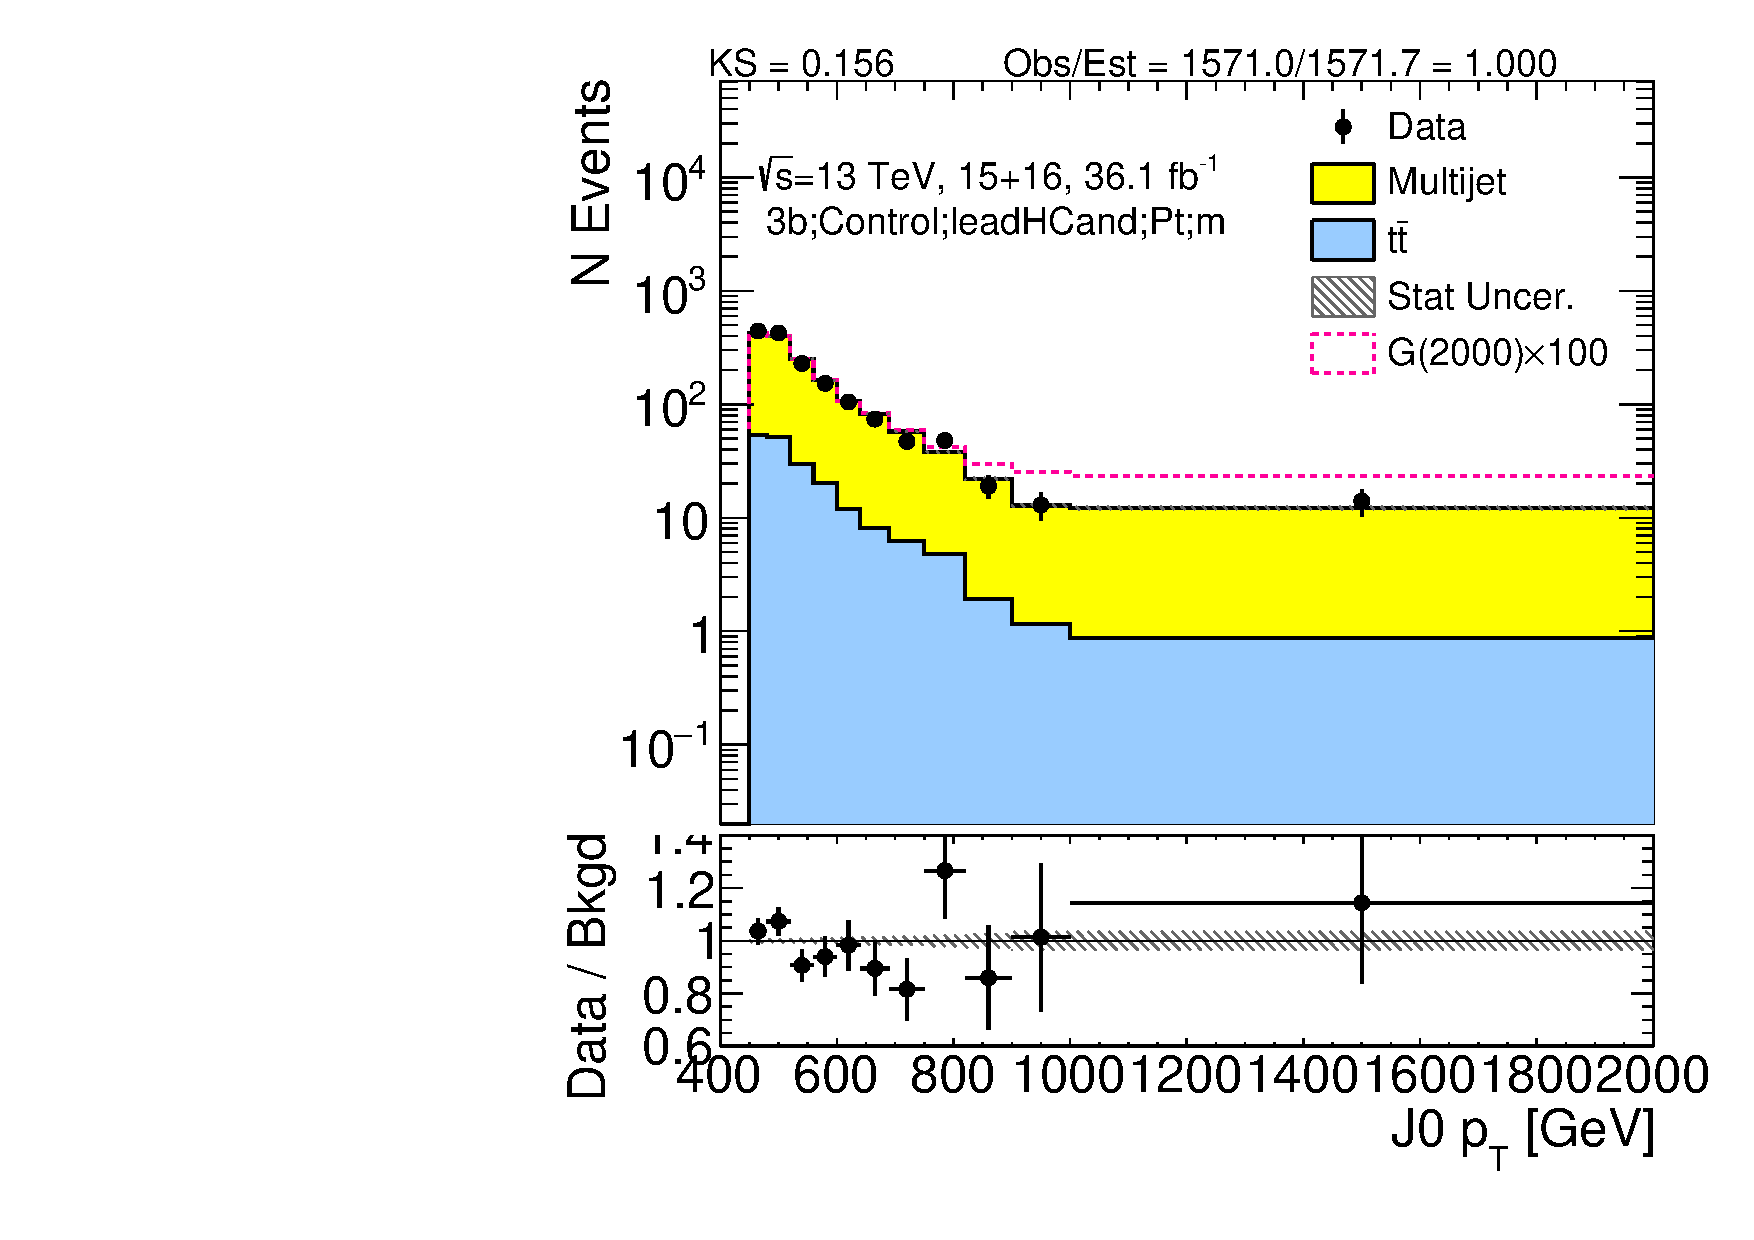
\includegraphics[width=0.33\textwidth, angle=270]{./figures/boosted/Control/Moriond_ThreeTag_Control_leadHCand_Pt_m_1.pdf}
0.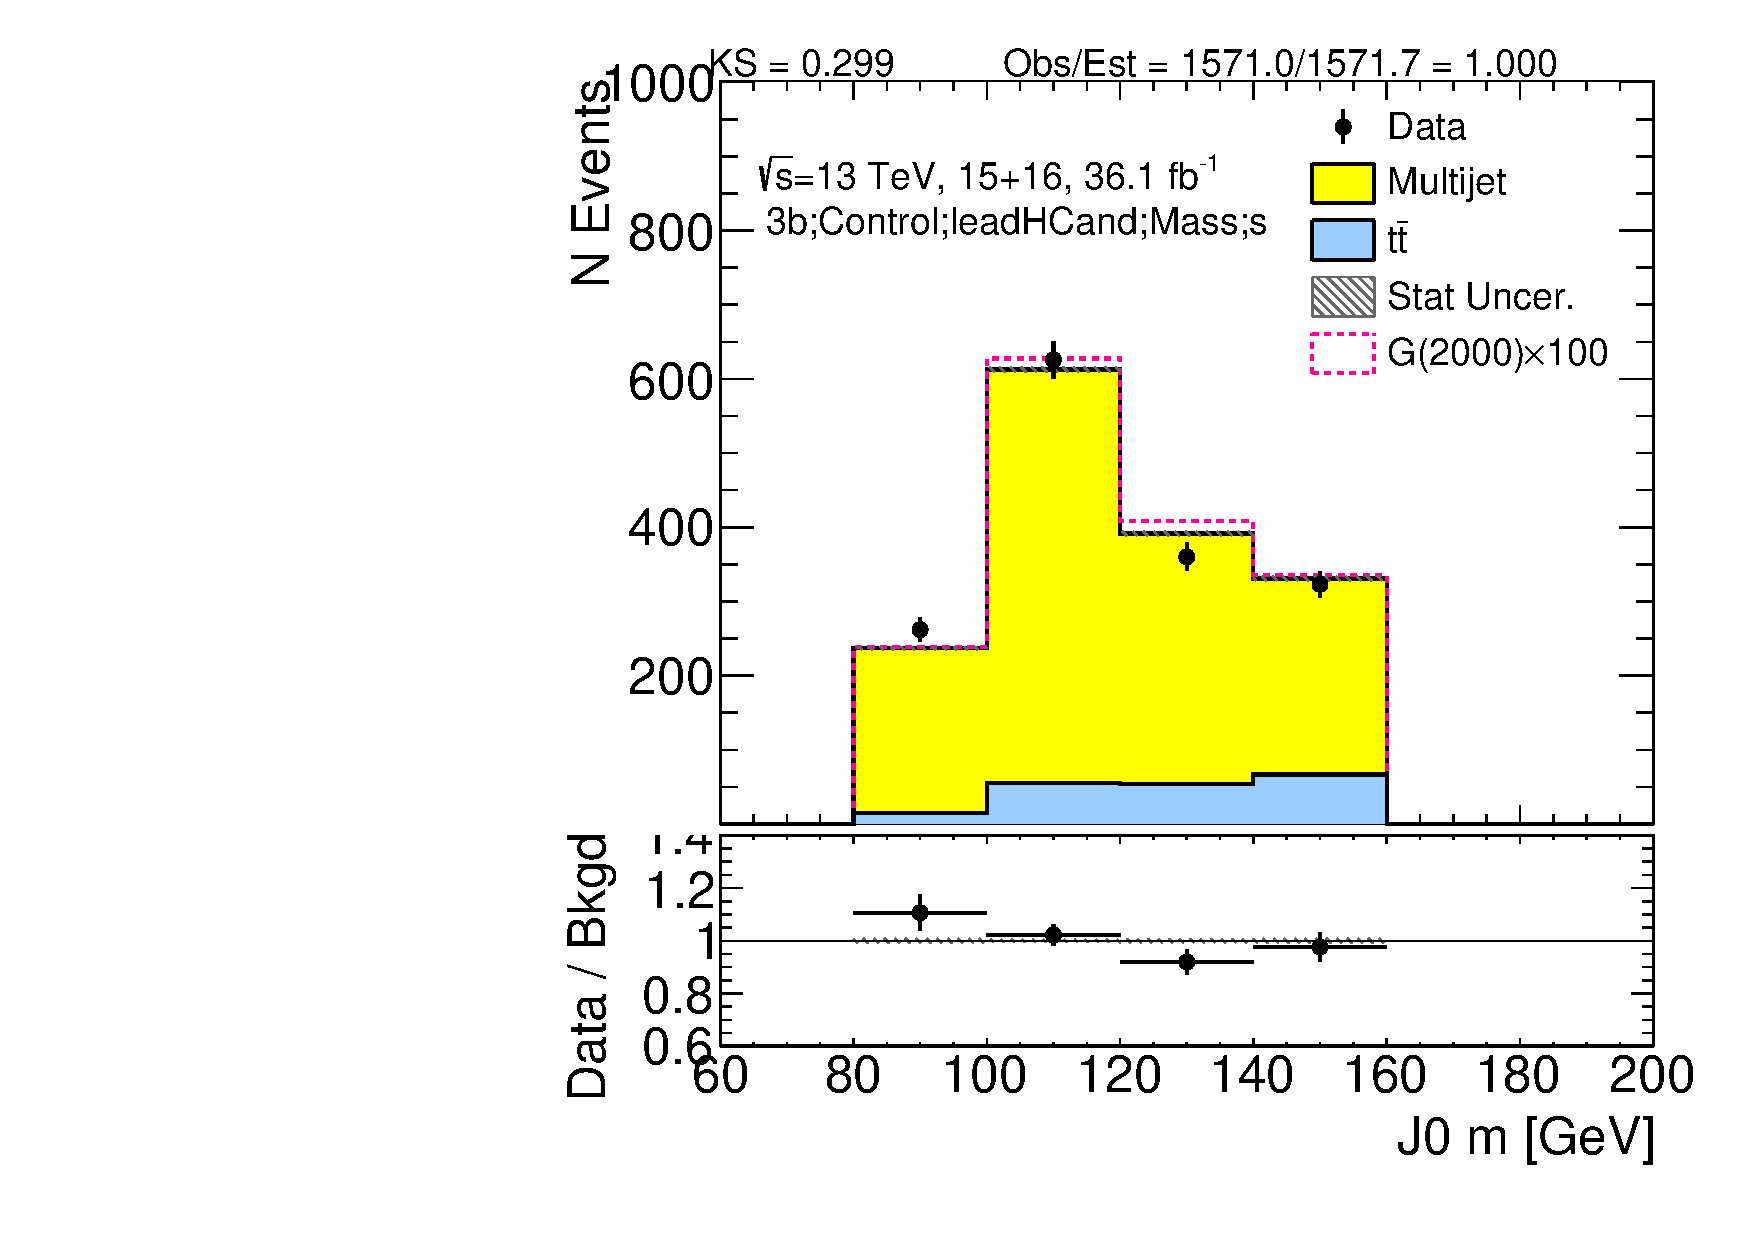
\includegraphics[width=0.33\textwidth, angle=270]{./figures/boosted/Control/Moriond_ThreeTag_Control_leadHCand_Mass_s.pdf}\\
0.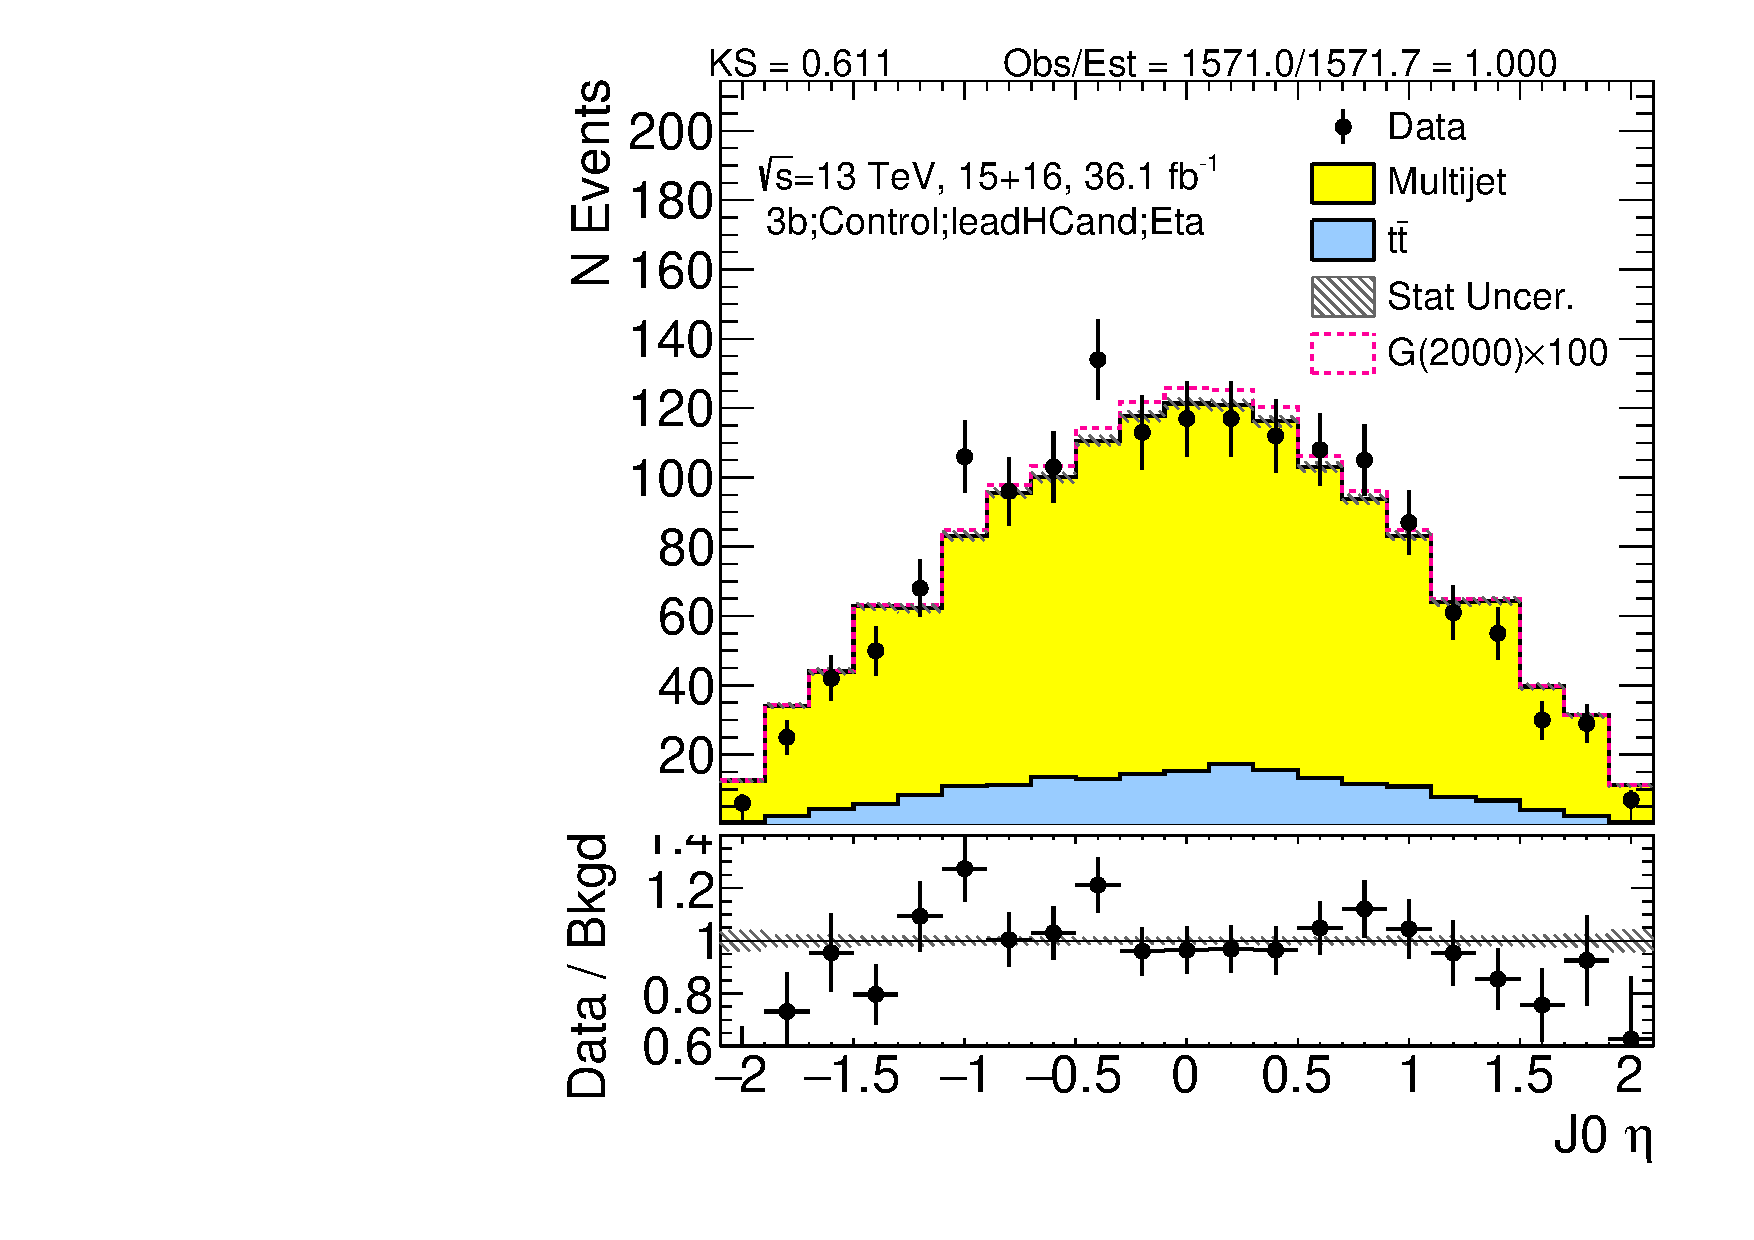
\includegraphics[width=0.33\textwidth, angle=270]{./figures/boosted/Control/Moriond_ThreeTag_Control_leadHCand_Eta.pdf}
0.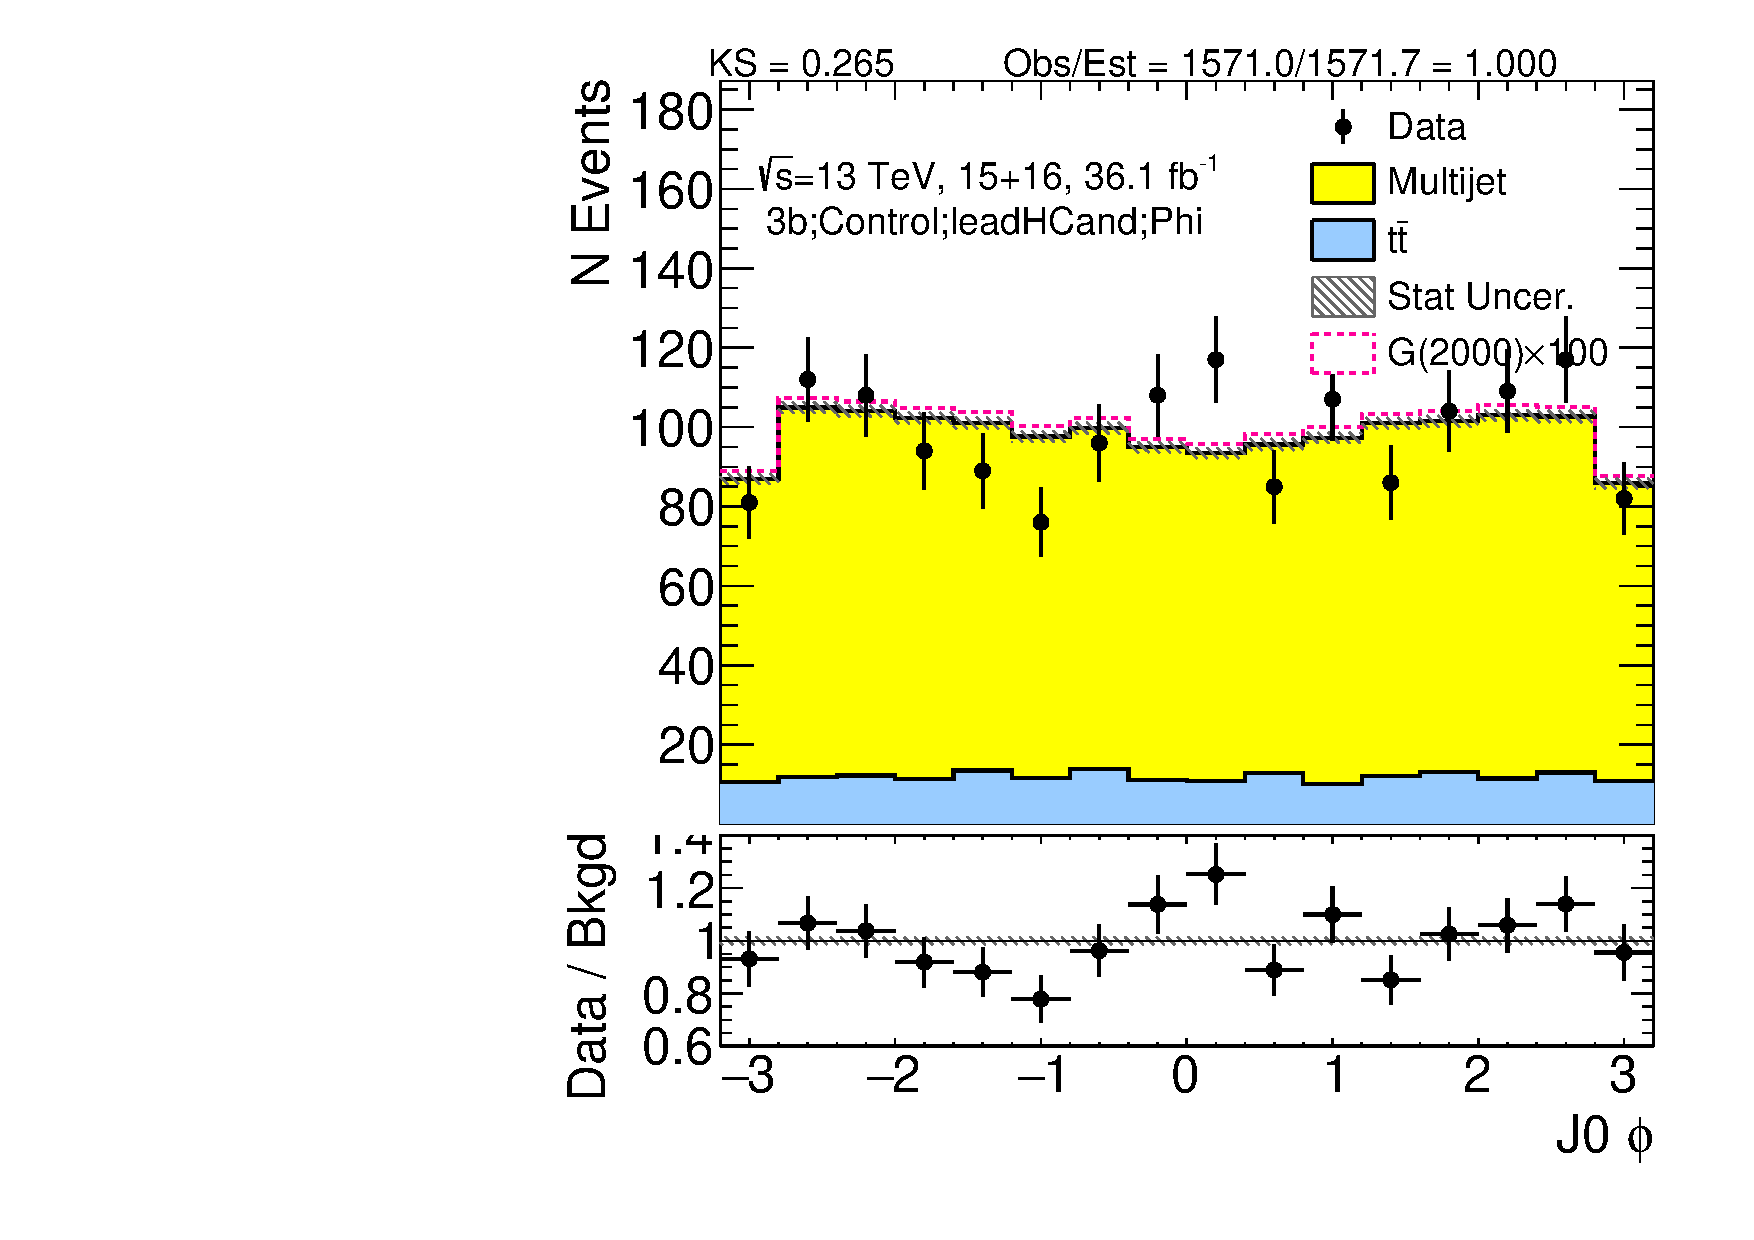
\includegraphics[width=0.33\textwidth, angle=270]{./figures/boosted/Control/Moriond_ThreeTag_Control_leadHCand_Phi.pdf}
  \caption{Kinematics of the lead large-$R$ jet in data and prediction in the sideband region after requiring 3 $b$-tags. The normalization agrees by construction, and the shapes are a feature of the prediction.}
  \label{fig:boosted-3b-control-ak10-lead}
\end{center}
\end{figure*}

\begin{figure*}[htbp!]
\begin{center}
0.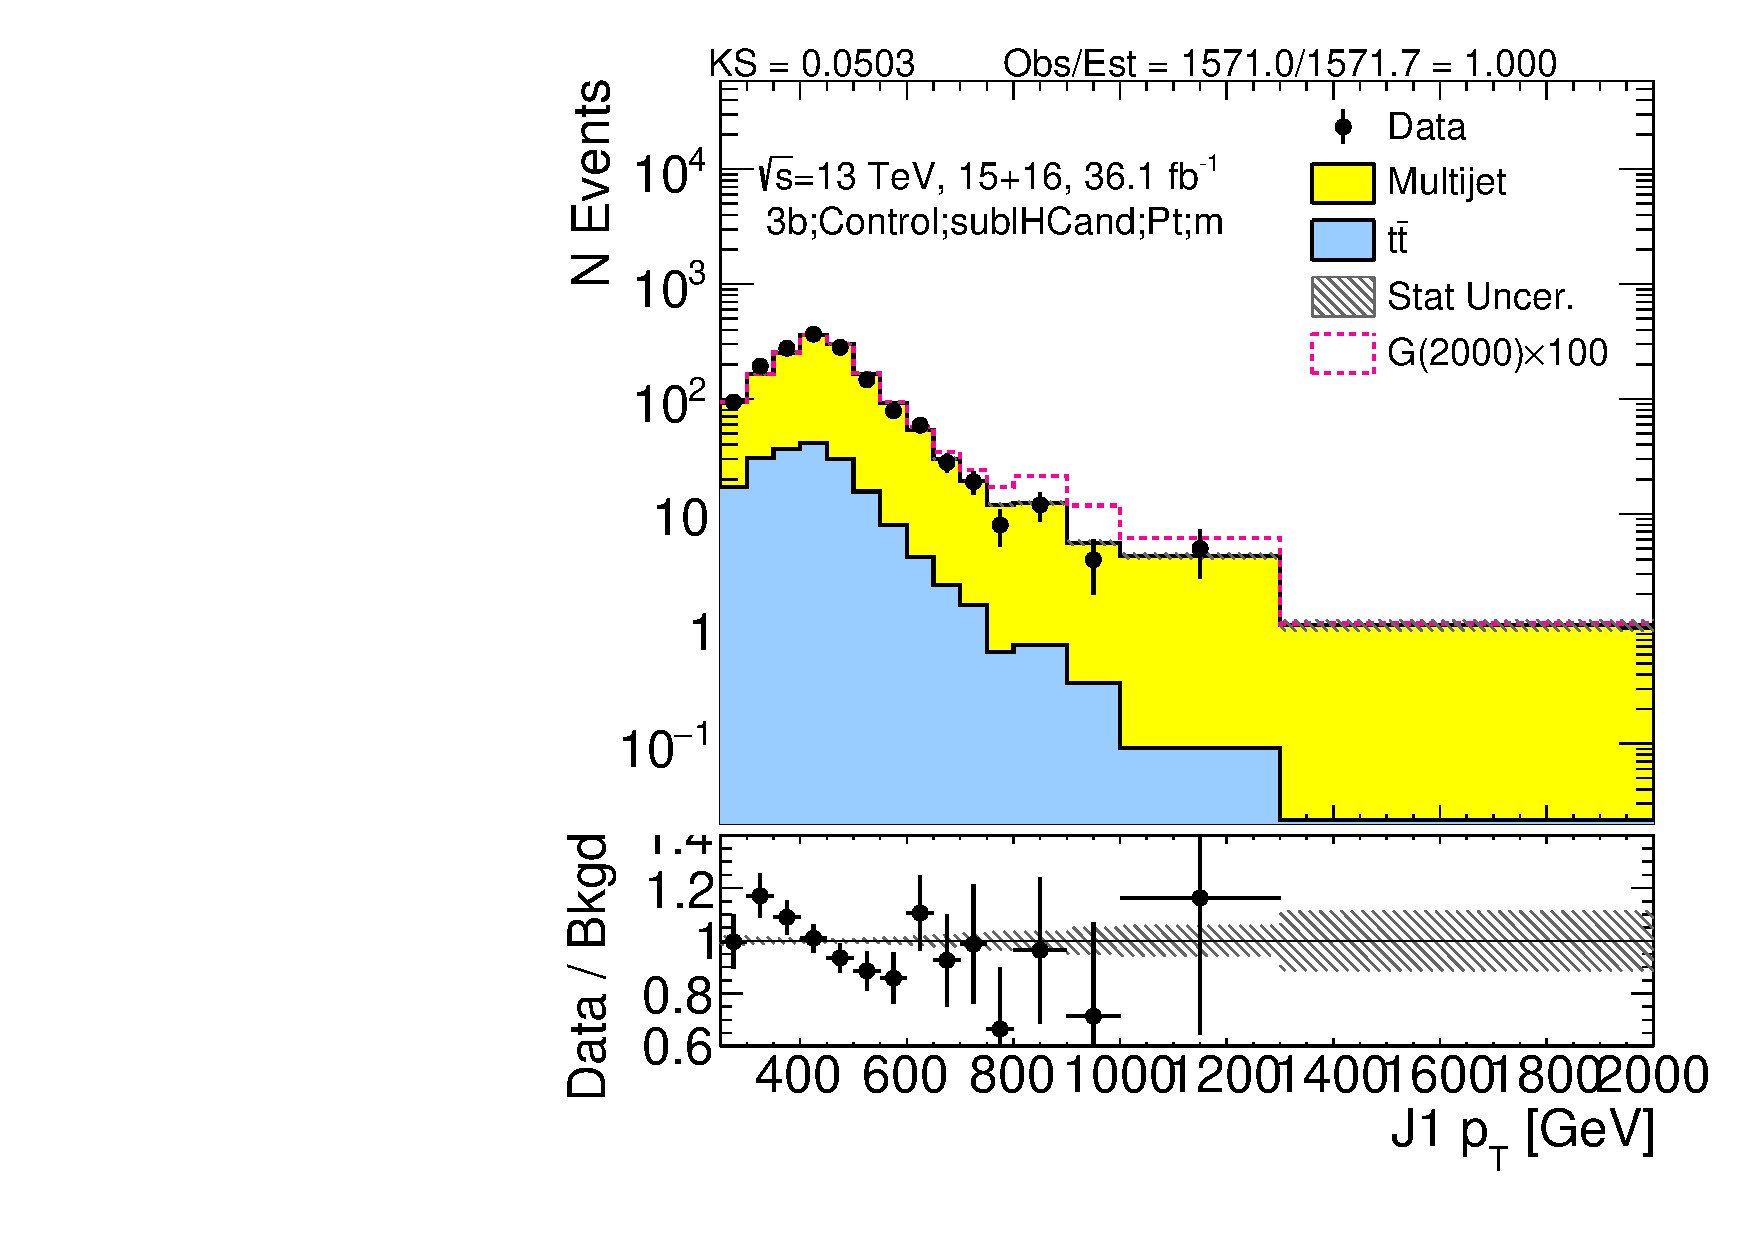
\includegraphics[width=0.33\textwidth, angle=270]{./figures/boosted/Control/Moriond_ThreeTag_Control_sublHCand_Pt_m_1.pdf}
0.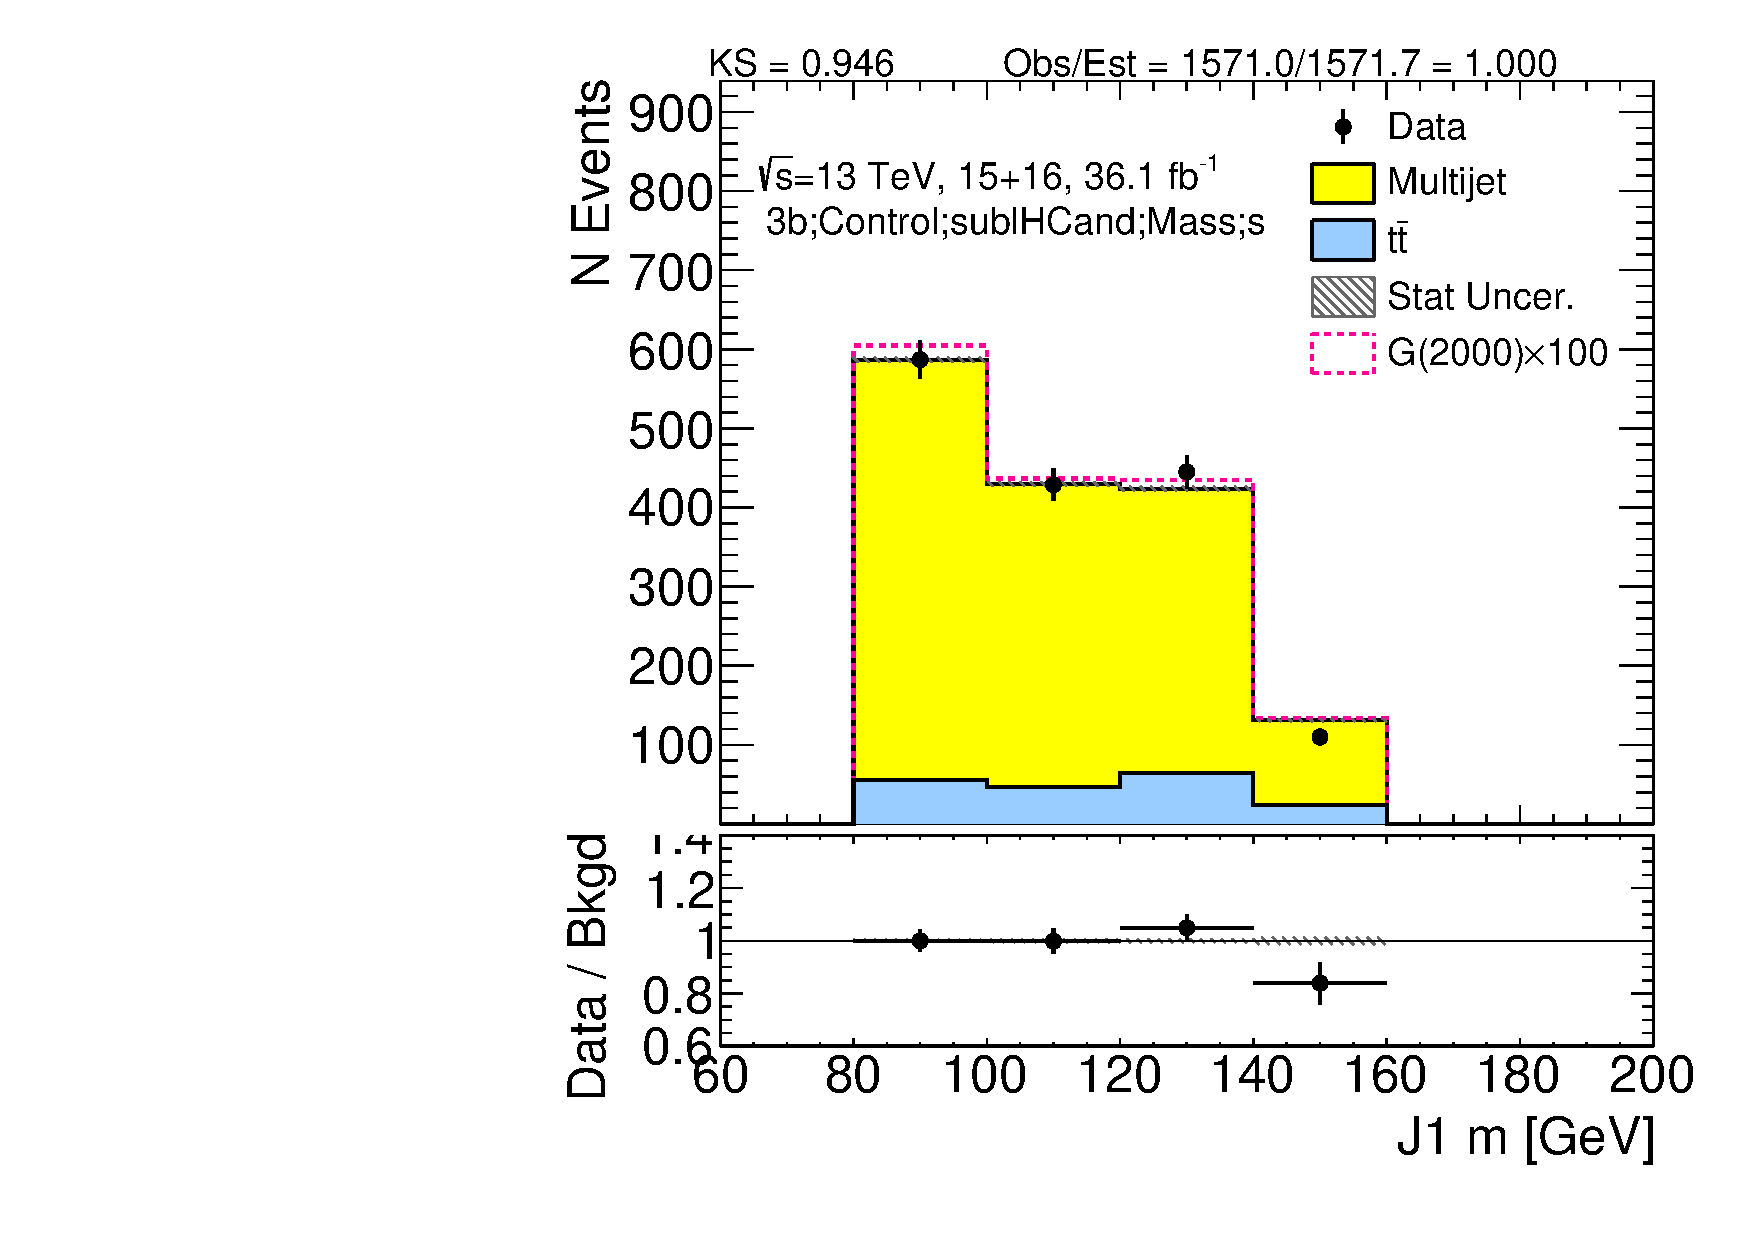
\includegraphics[width=0.33\textwidth, angle=270]{./figures/boosted/Control/Moriond_ThreeTag_Control_sublHCand_Mass_s.pdf}\\
0.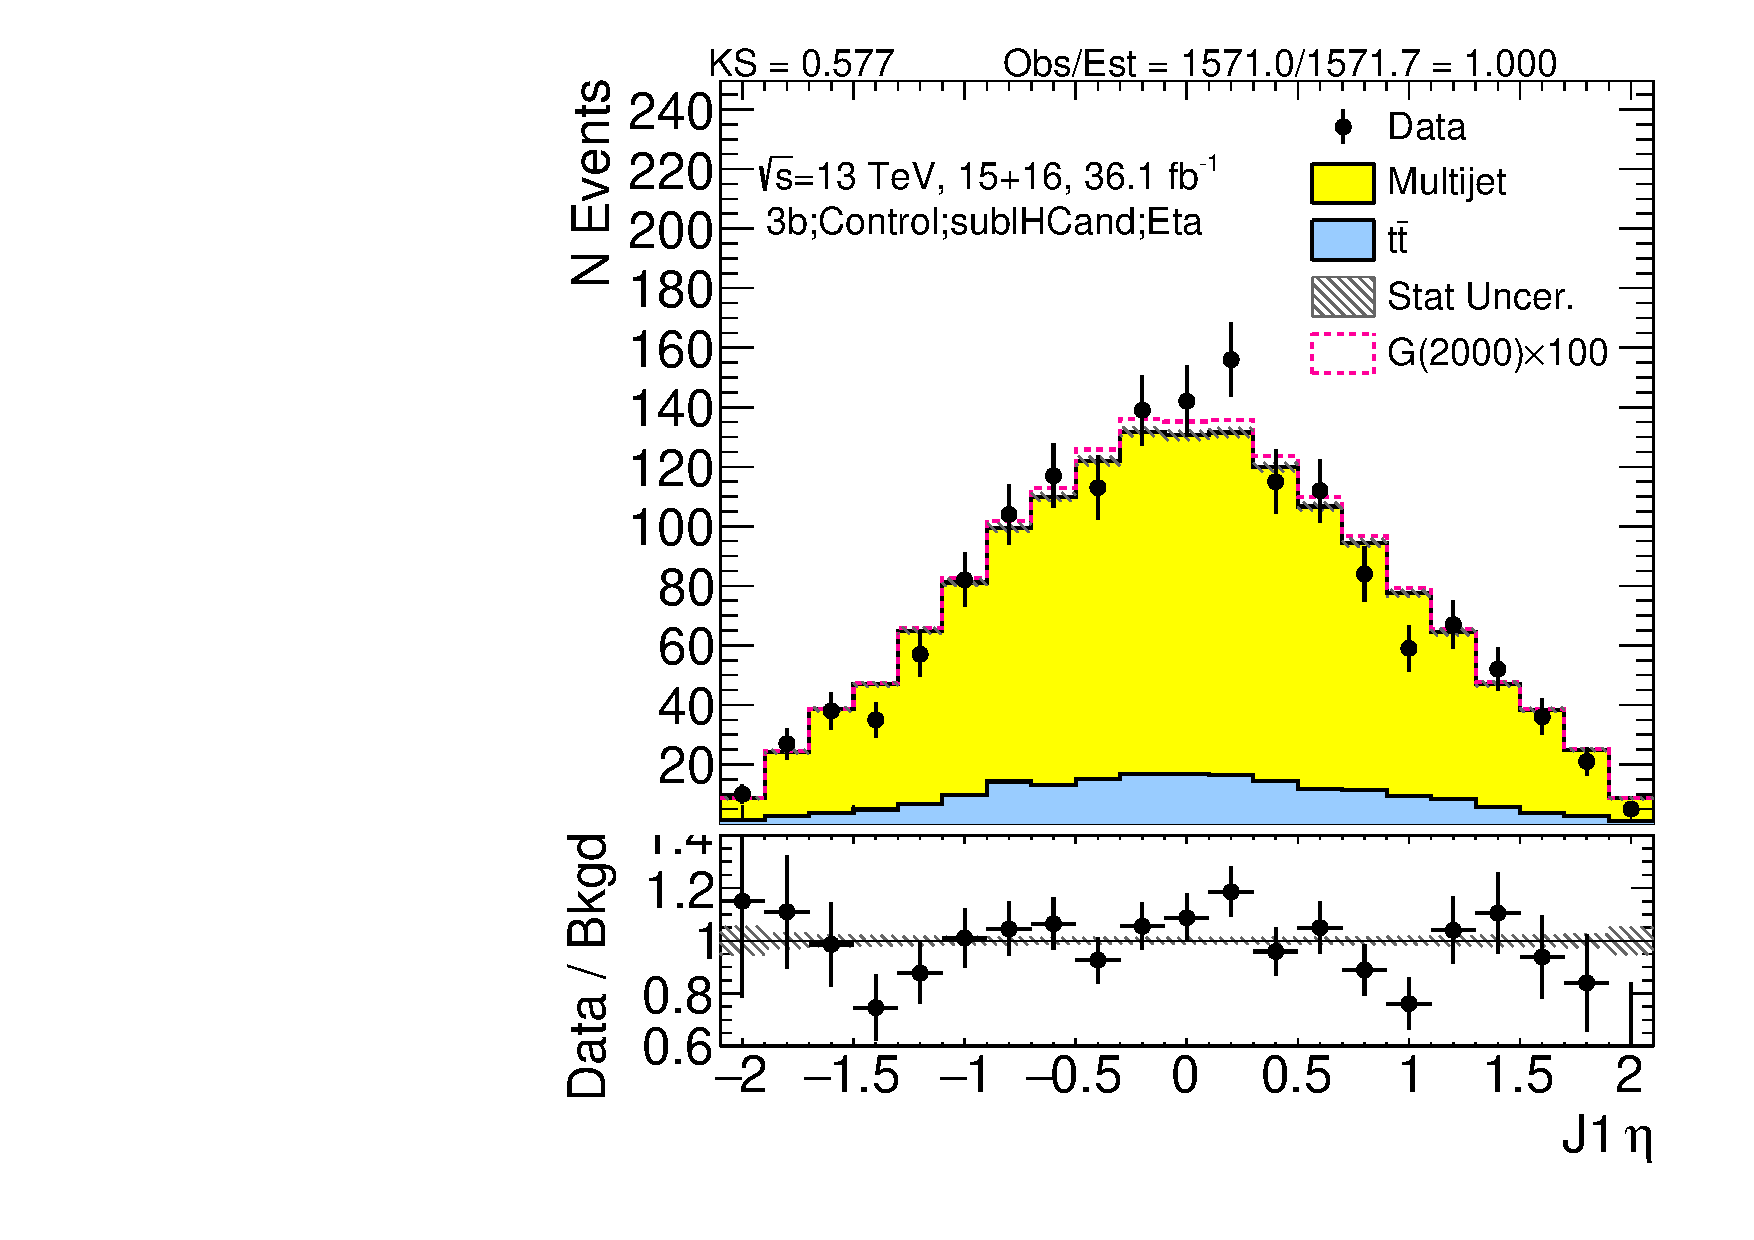
\includegraphics[width=0.33\textwidth, angle=270]{./figures/boosted/Control/Moriond_ThreeTag_Control_sublHCand_Eta.pdf}
0.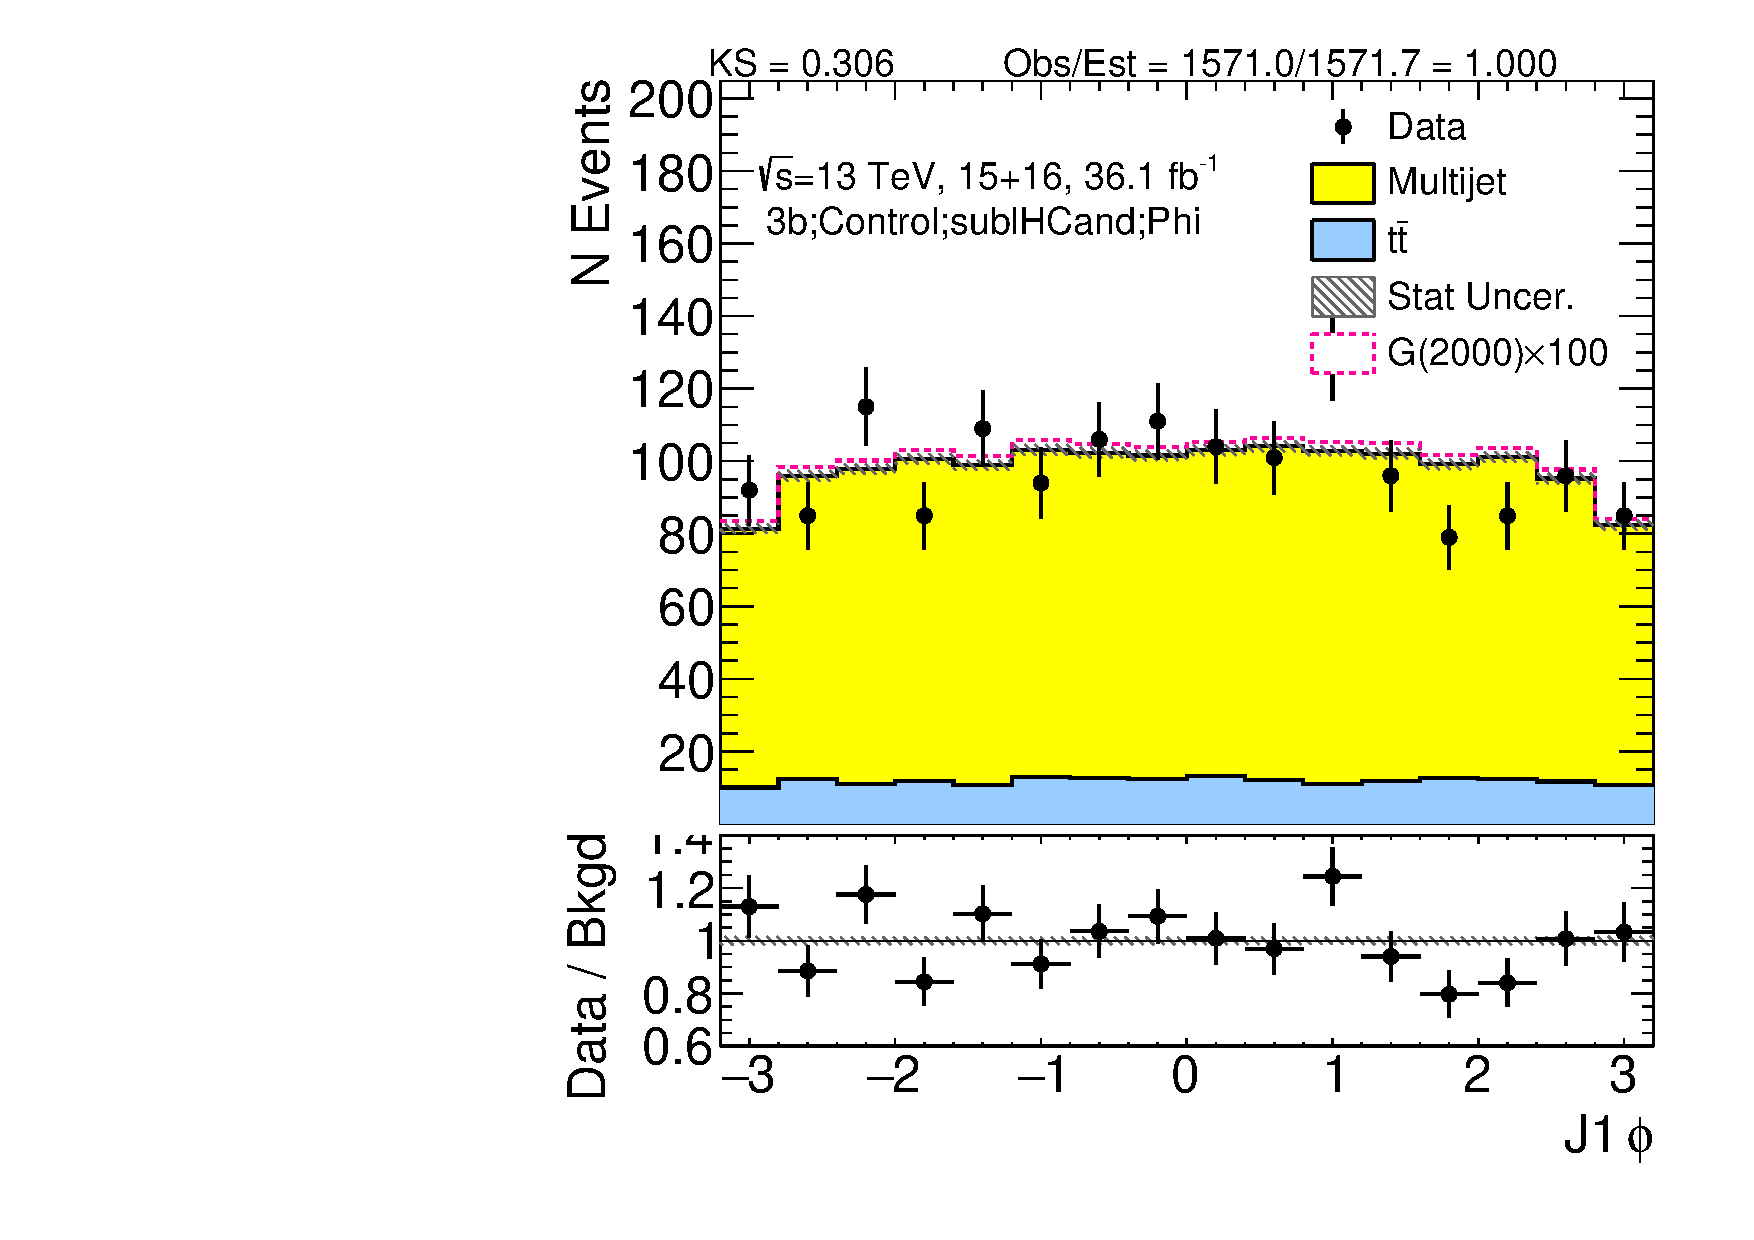
\includegraphics[width=0.33\textwidth, angle=270]{./figures/boosted/Control/Moriond_ThreeTag_Control_sublHCand_Phi.pdf}
  \caption{Kinematics of the sub-lead large-$R$ jet in data and prediction in the sideband region after requiring 3 $b$-tags. The normalization agrees by construction, and the shapes are a feature of the prediction.}
  \label{fig:boosted-3b-control-ak10-subl}
\end{center}
\end{figure*}

\begin{figure*}[htbp!]
\begin{center}
0.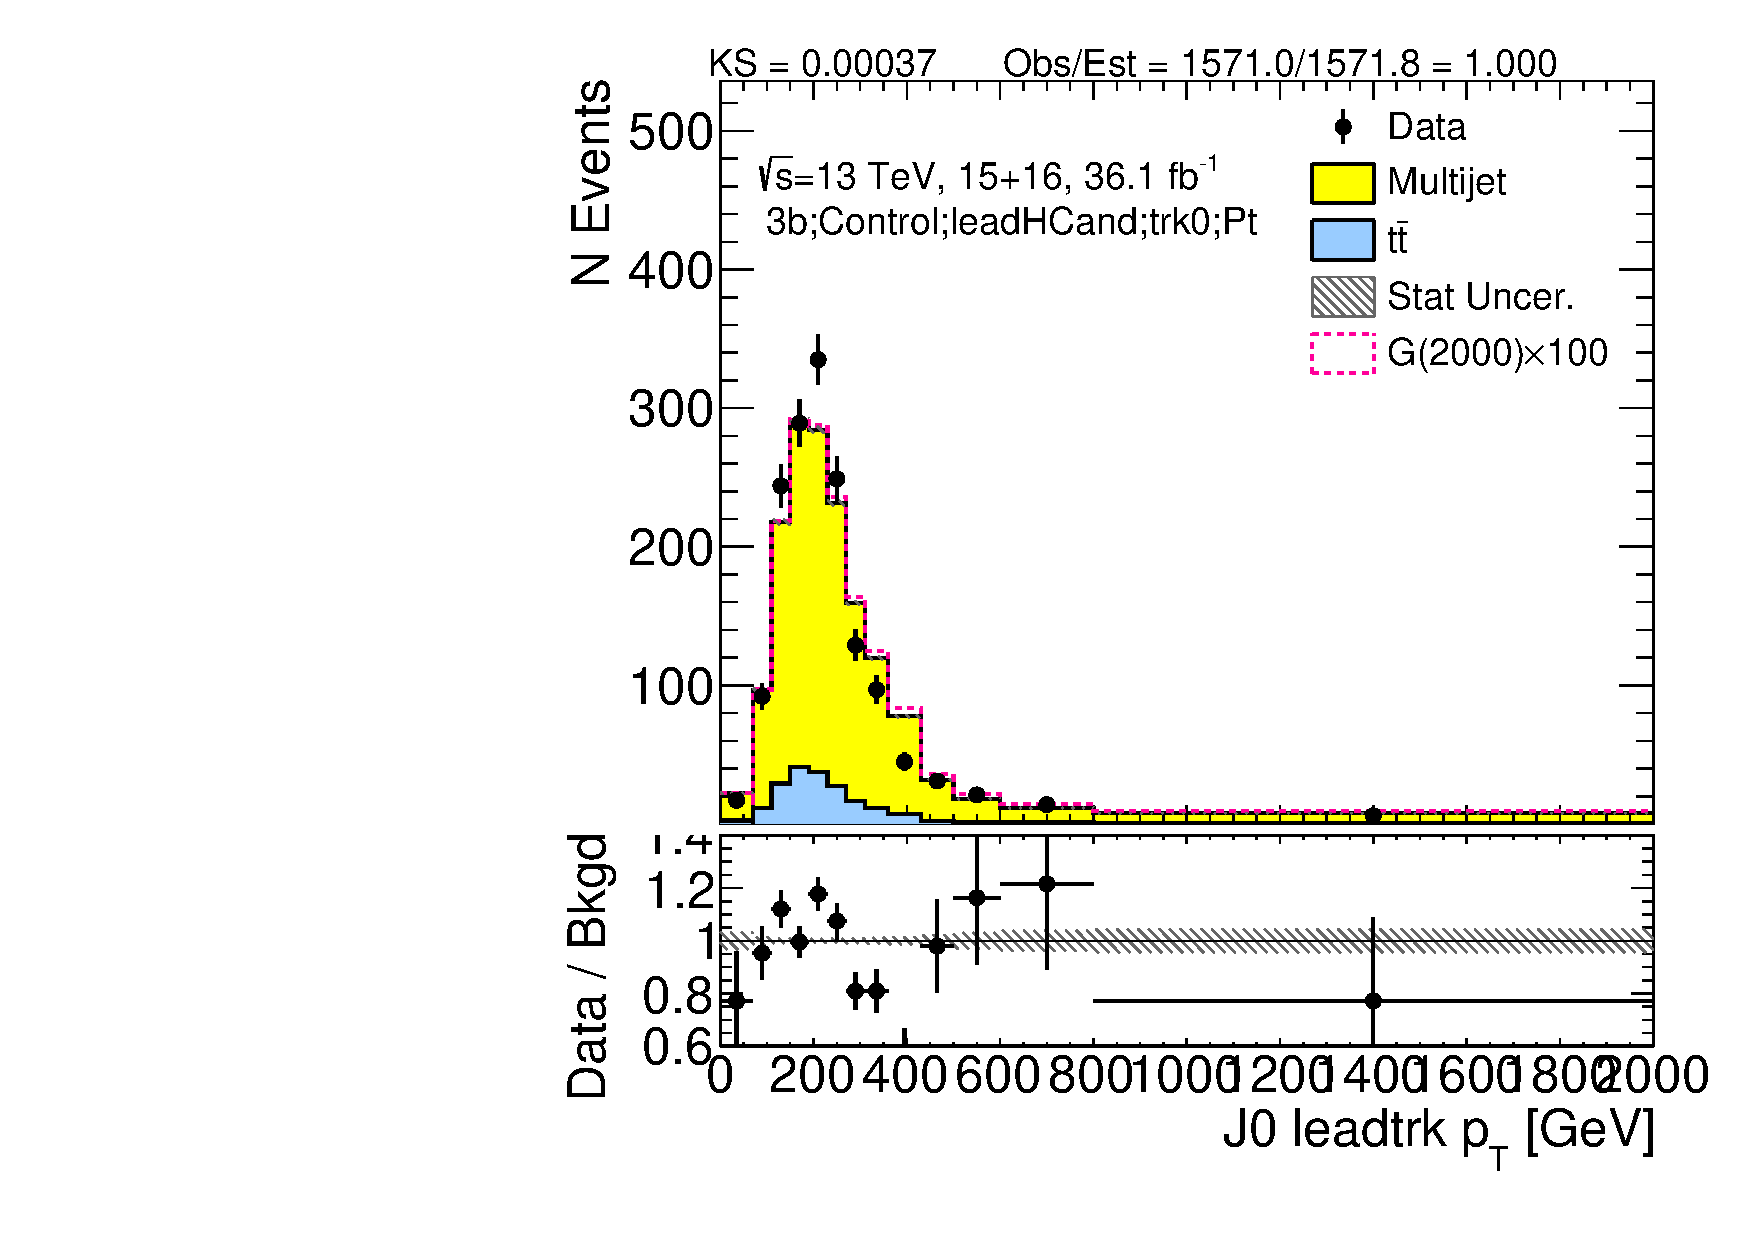
\includegraphics[width=0.33\textwidth, angle=270]{./figures/boosted/Control/Moriond_ThreeTag_Control_leadHCand_trk0_Pt.pdf}
0.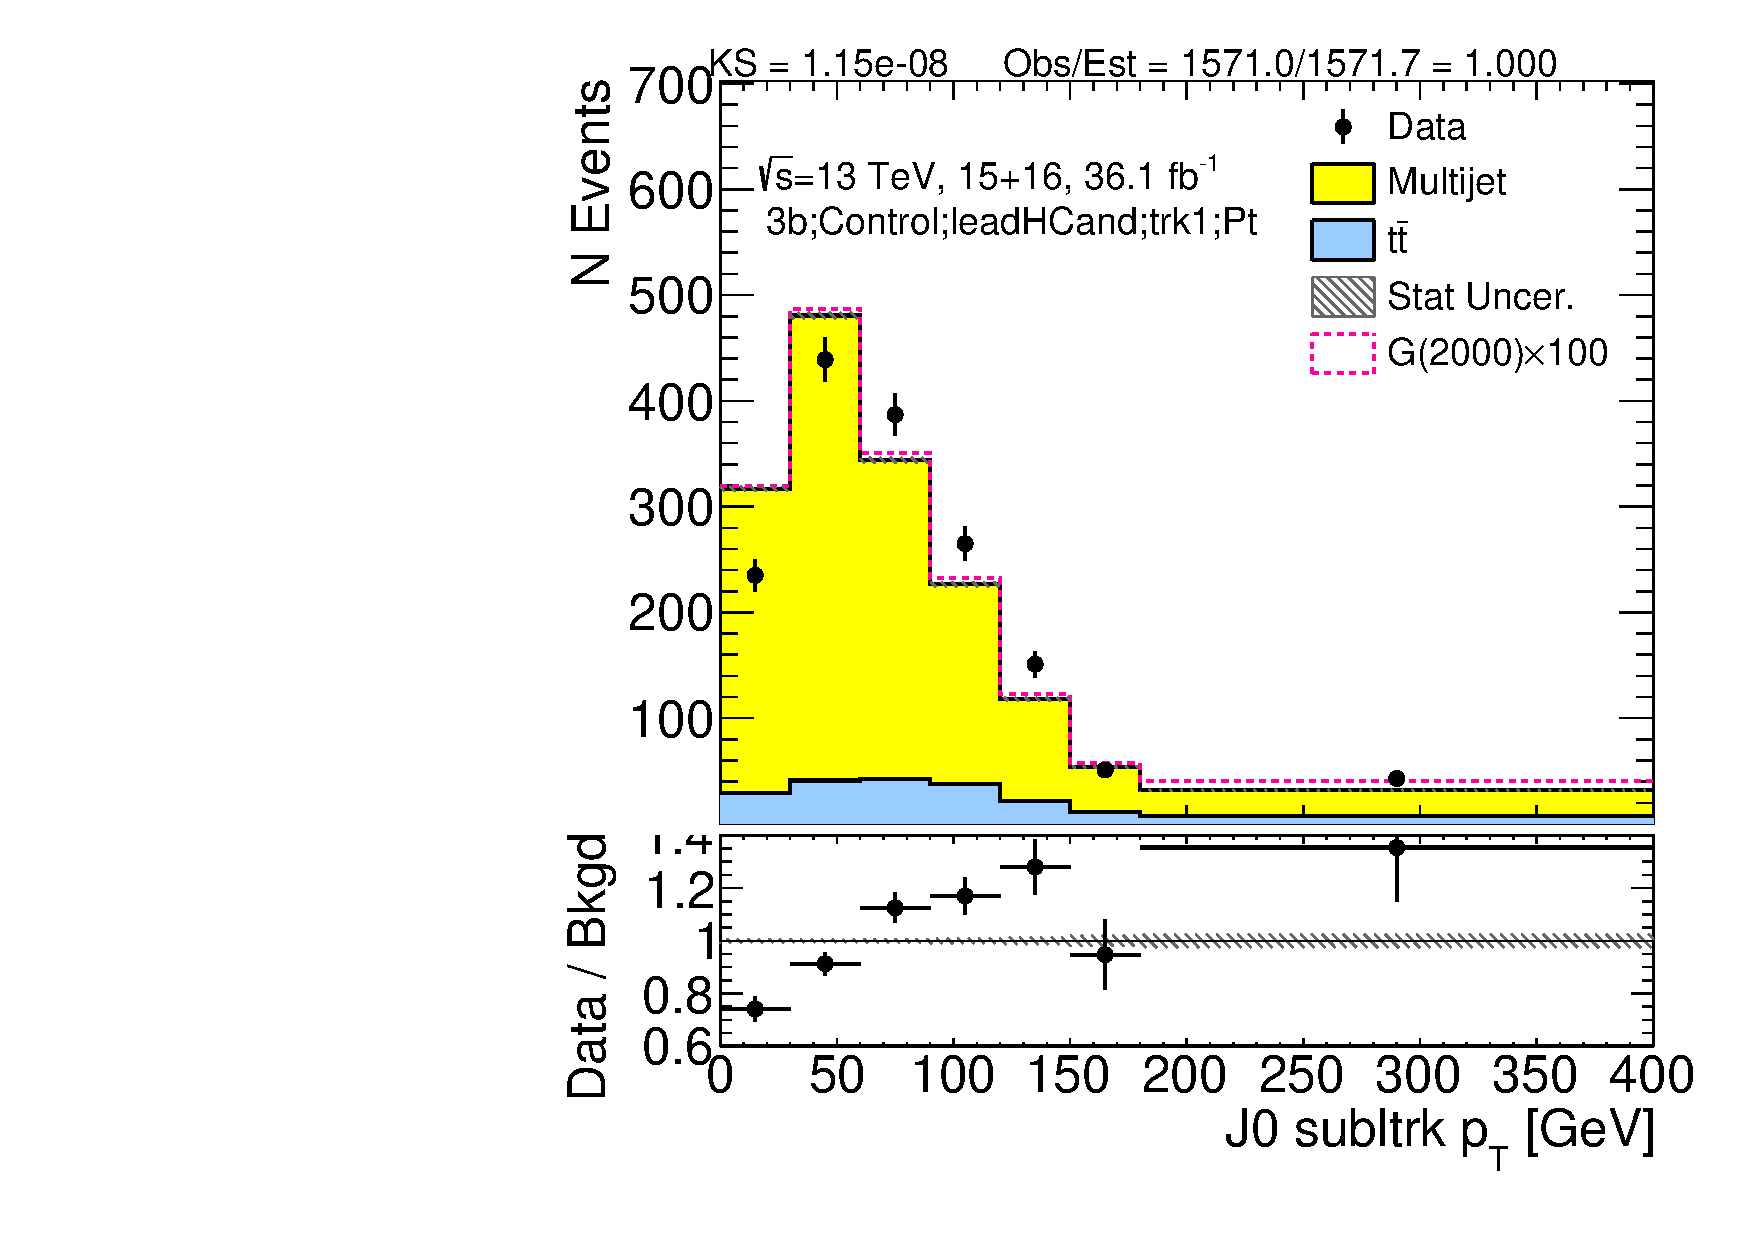
\includegraphics[width=0.33\textwidth, angle=270]{./figures/boosted/Control/Moriond_ThreeTag_Control_leadHCand_trk1_Pt.pdf}\\
0.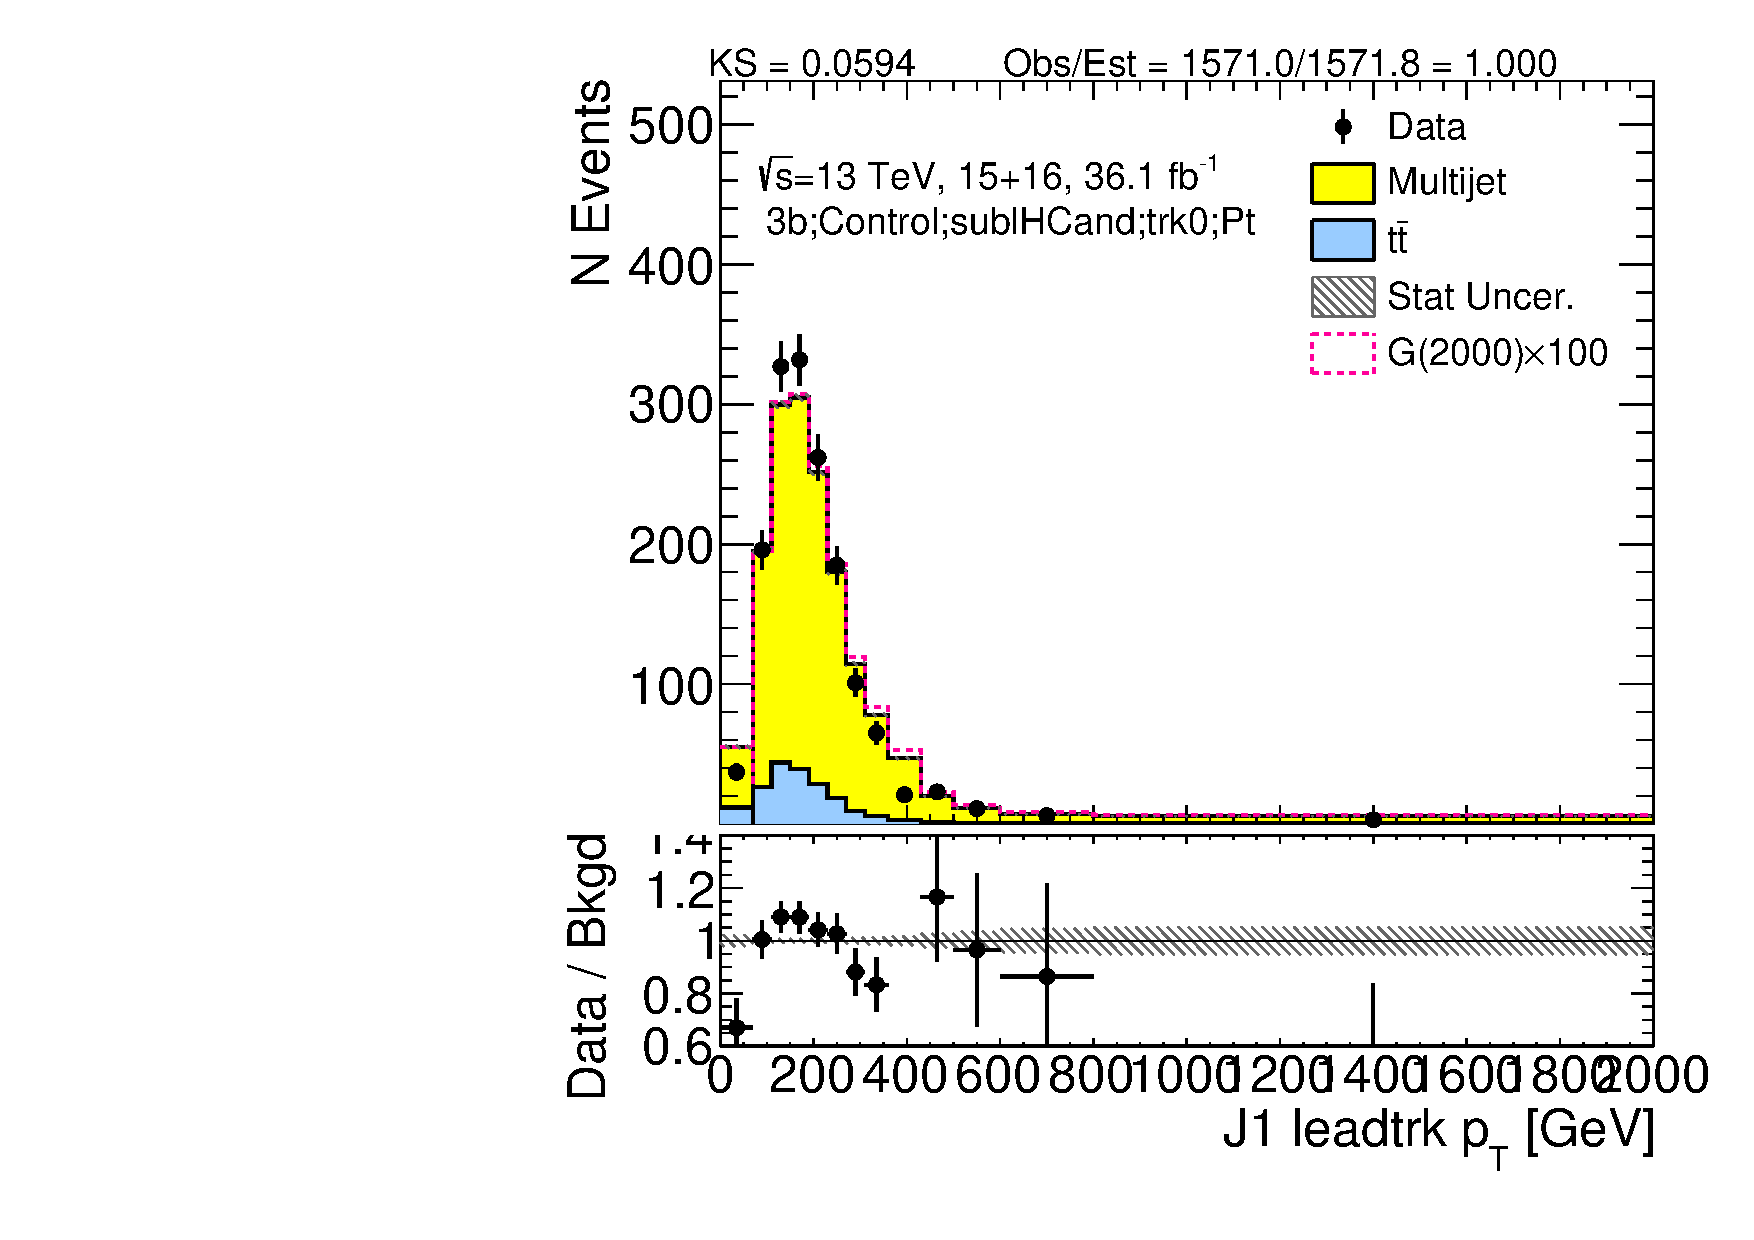
\includegraphics[width=0.33\textwidth, angle=270]{./figures/boosted/Control/Moriond_ThreeTag_Control_sublHCand_trk0_Pt.pdf}
0.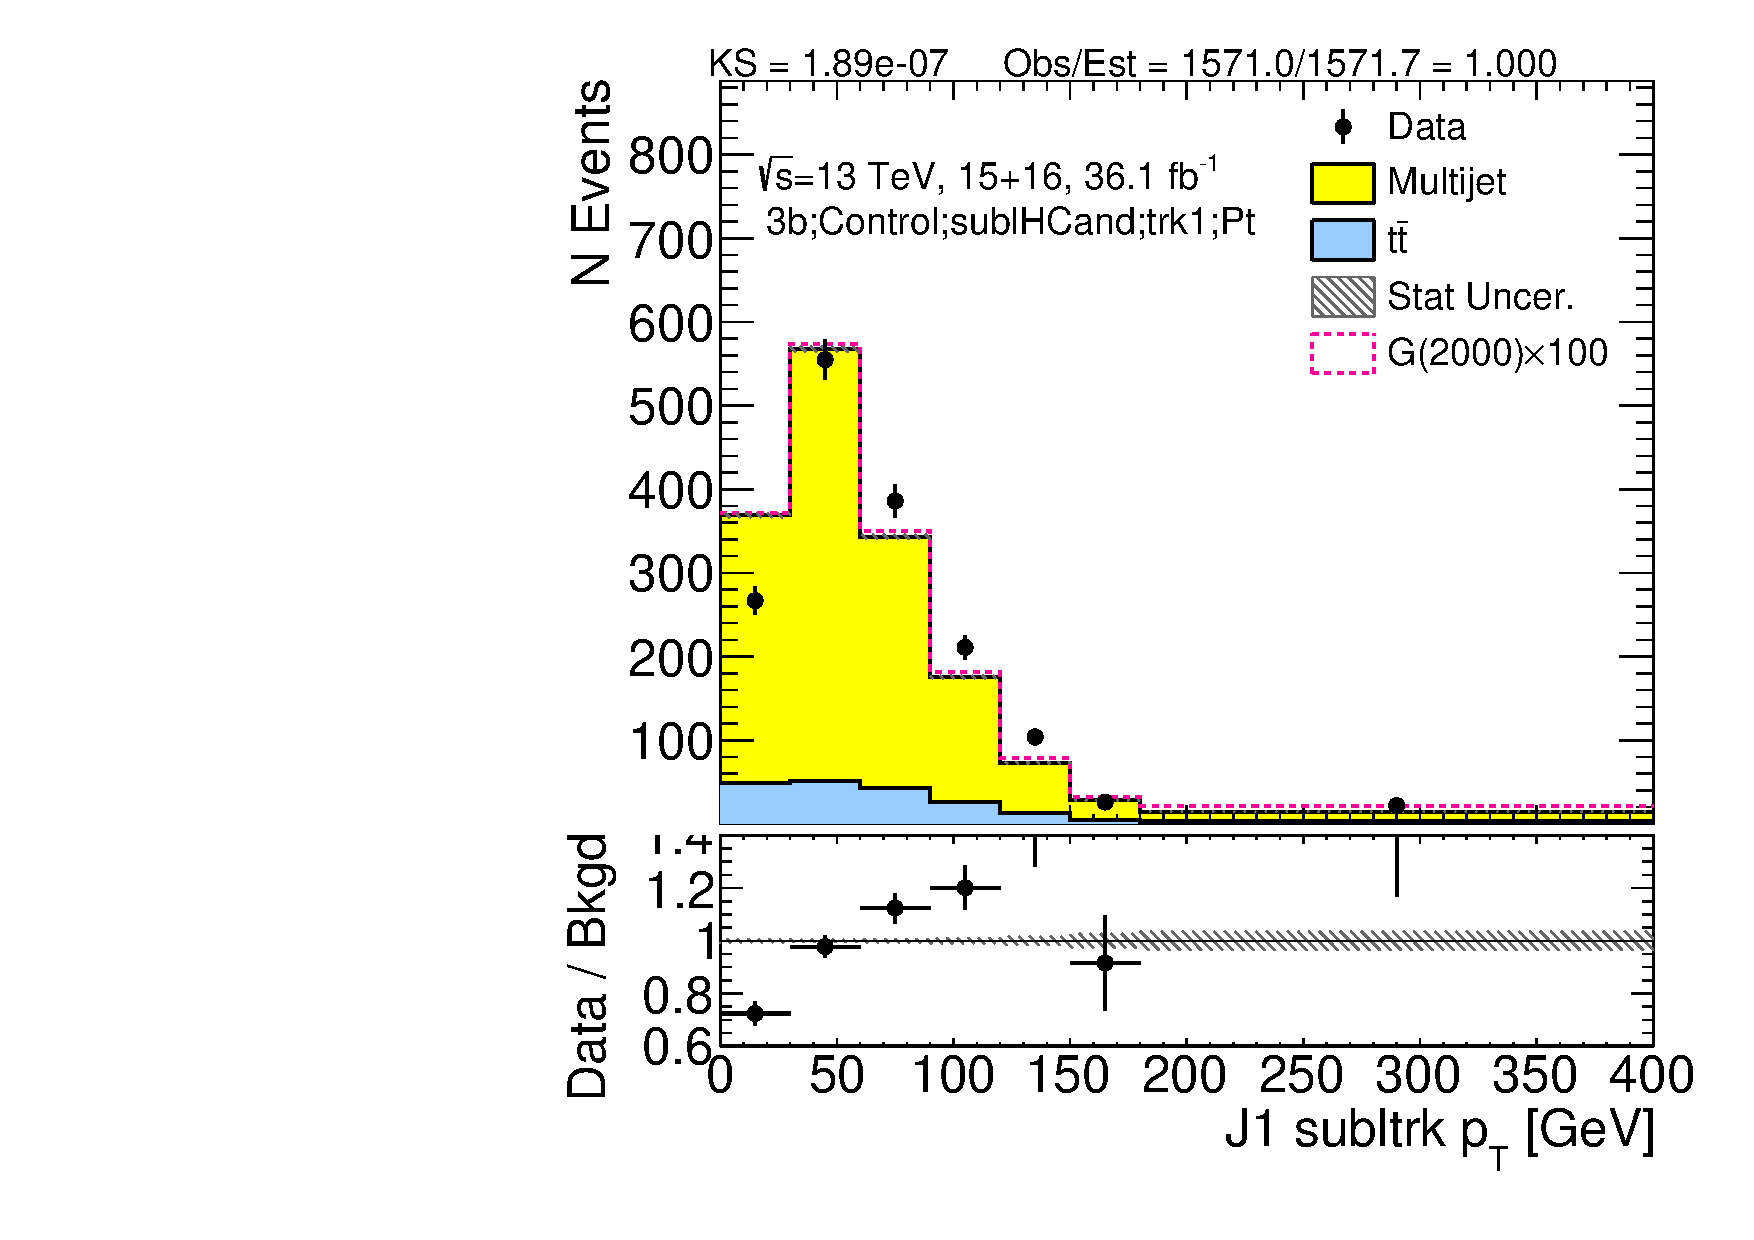
\includegraphics[width=0.33\textwidth, angle=270]{./figures/boosted/Control/Moriond_ThreeTag_Control_sublHCand_trk1_Pt.pdf}\\
0.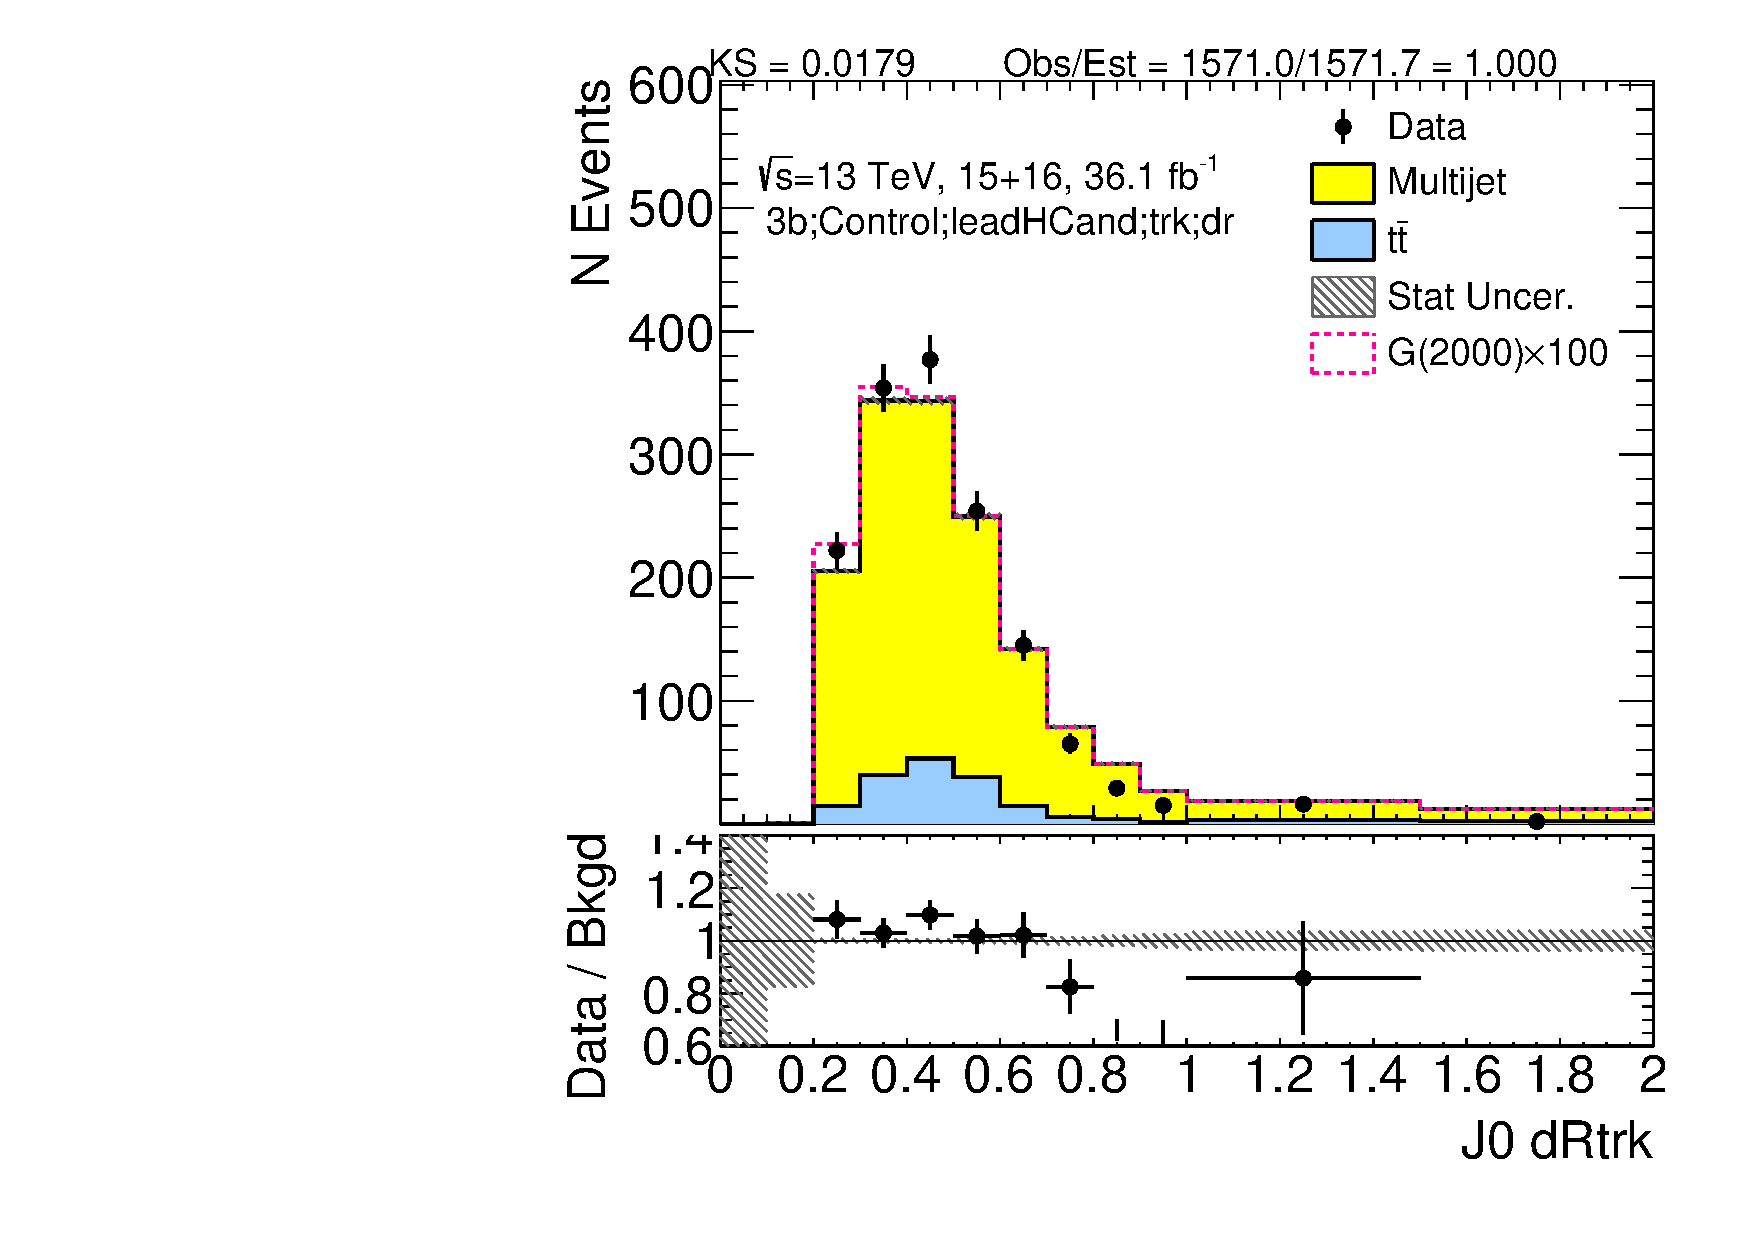
\includegraphics[width=0.33\textwidth, angle=270]{./figures/boosted/Control/Moriond_ThreeTag_Control_leadHCand_trk_dr.pdf}
0.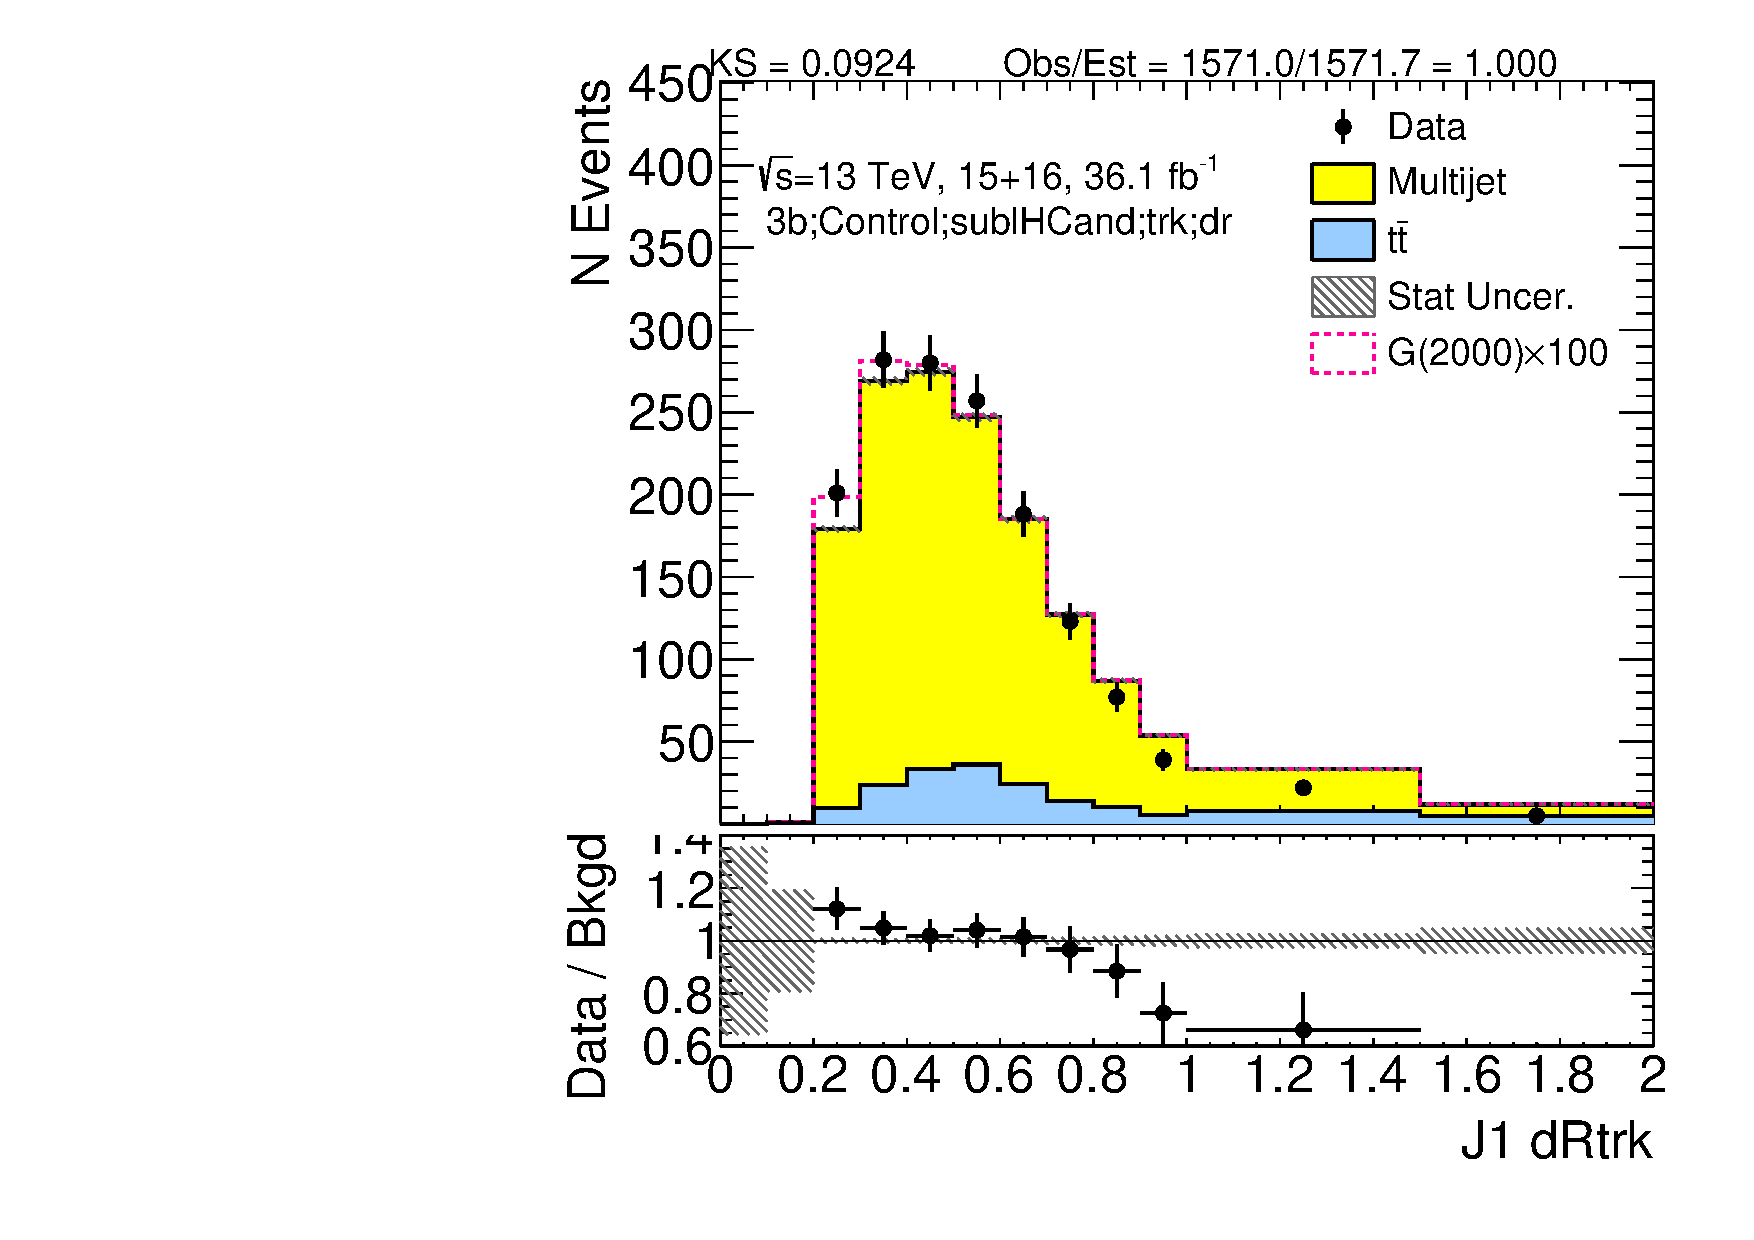
\includegraphics[width=0.33\textwidth, angle=270]{./figures/boosted/Control/Moriond_ThreeTag_Control_sublHCand_trk_dr.pdf}
  \caption{First two rows show the kinematics of the lead (left) and sub-lead (right) small-$R$ track jets associated to the lead (first-row) and sub-lead (second-row) large-$R$ jet in data and prediction in the sideband region after requiring 3 $b$-tags. Third row shows the $\Delta R$ between two leading small-$R$ track-jets associated to the leading (left) and sub-leading (right) large-$R$ jet. The normalization agrees by construction, and the shapes are a feature of the prediction. }
  \label{fig:boosted-3b-control-ak2}
\end{center}
\end{figure*}


\begin{figure*}[htbp!]
\begin{center}
0.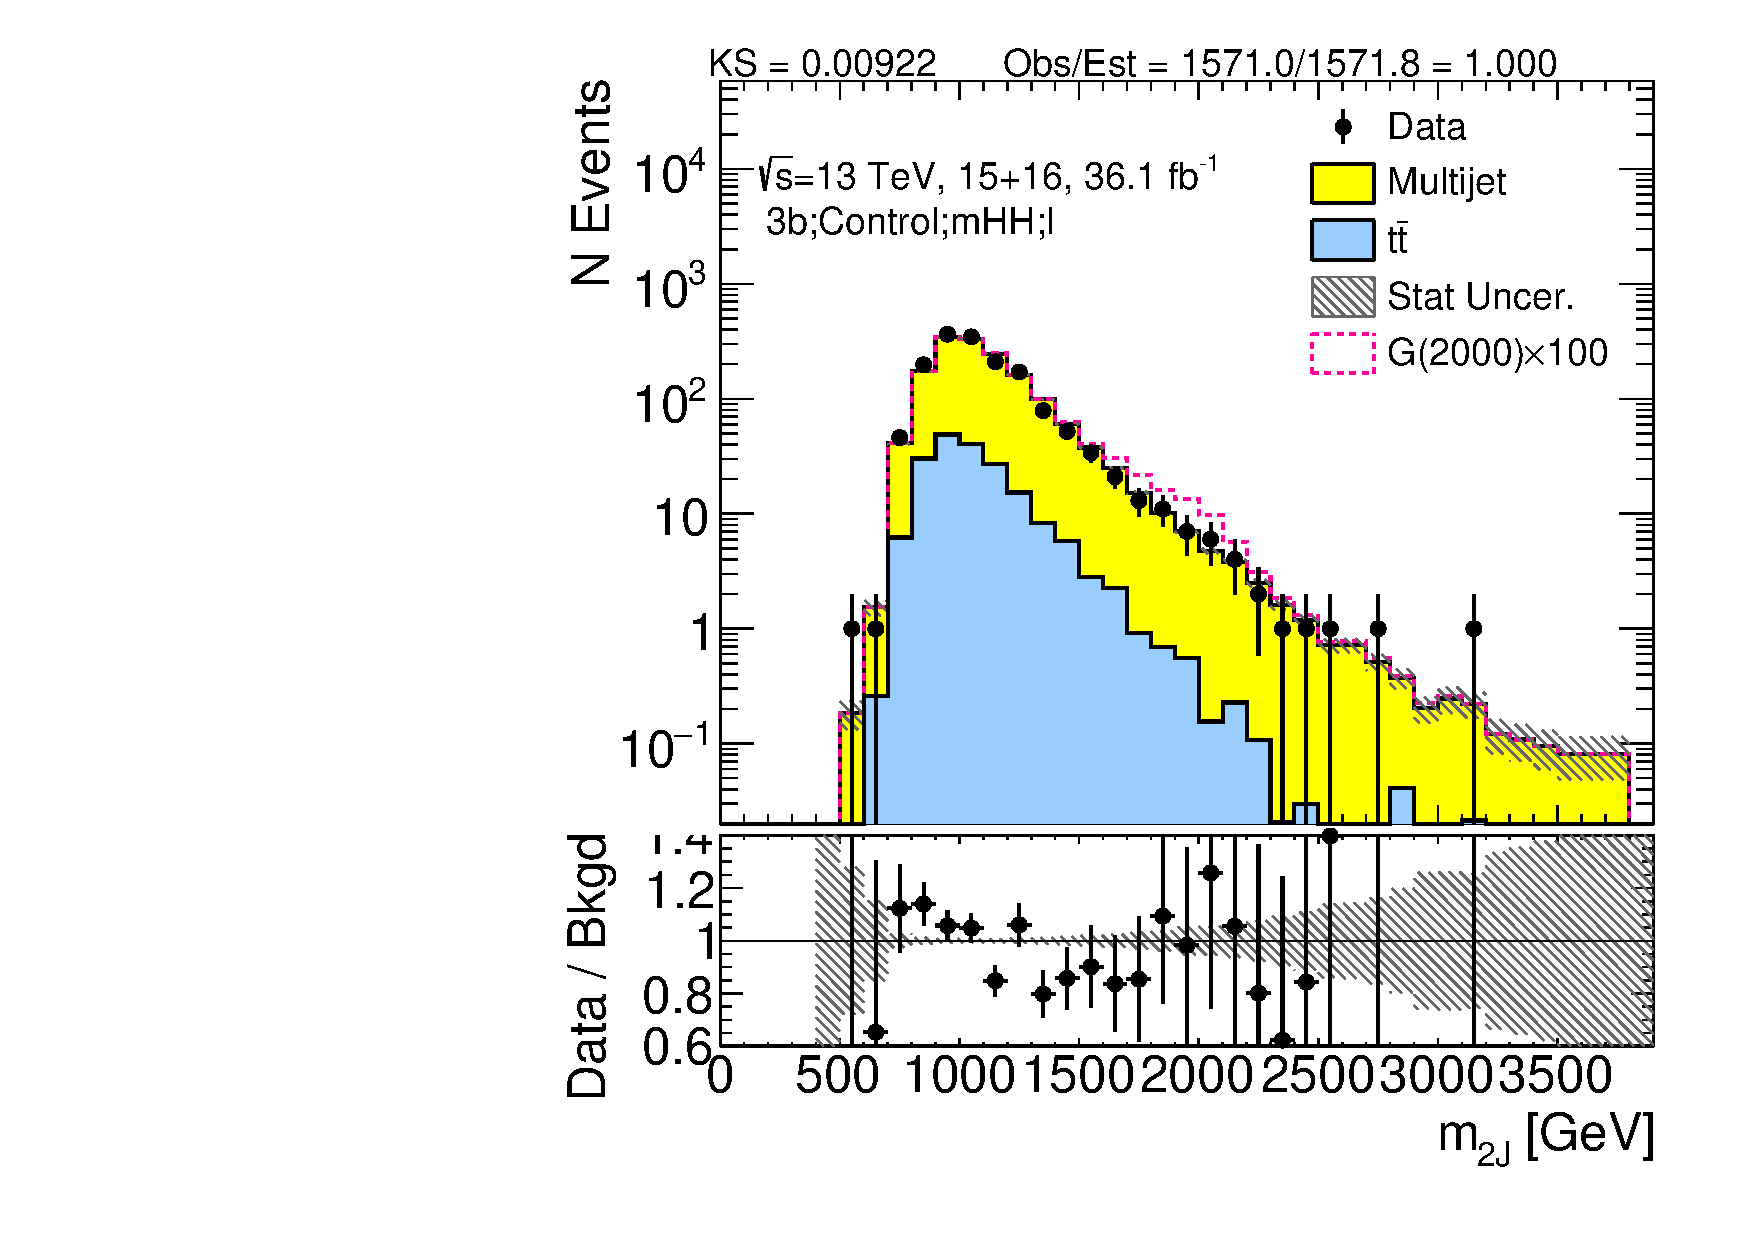
\includegraphics[width=0.33\textwidth, angle=270]{./figures/boosted/Control/Moriond_ThreeTag_Control_mHH_l_1.pdf}
0.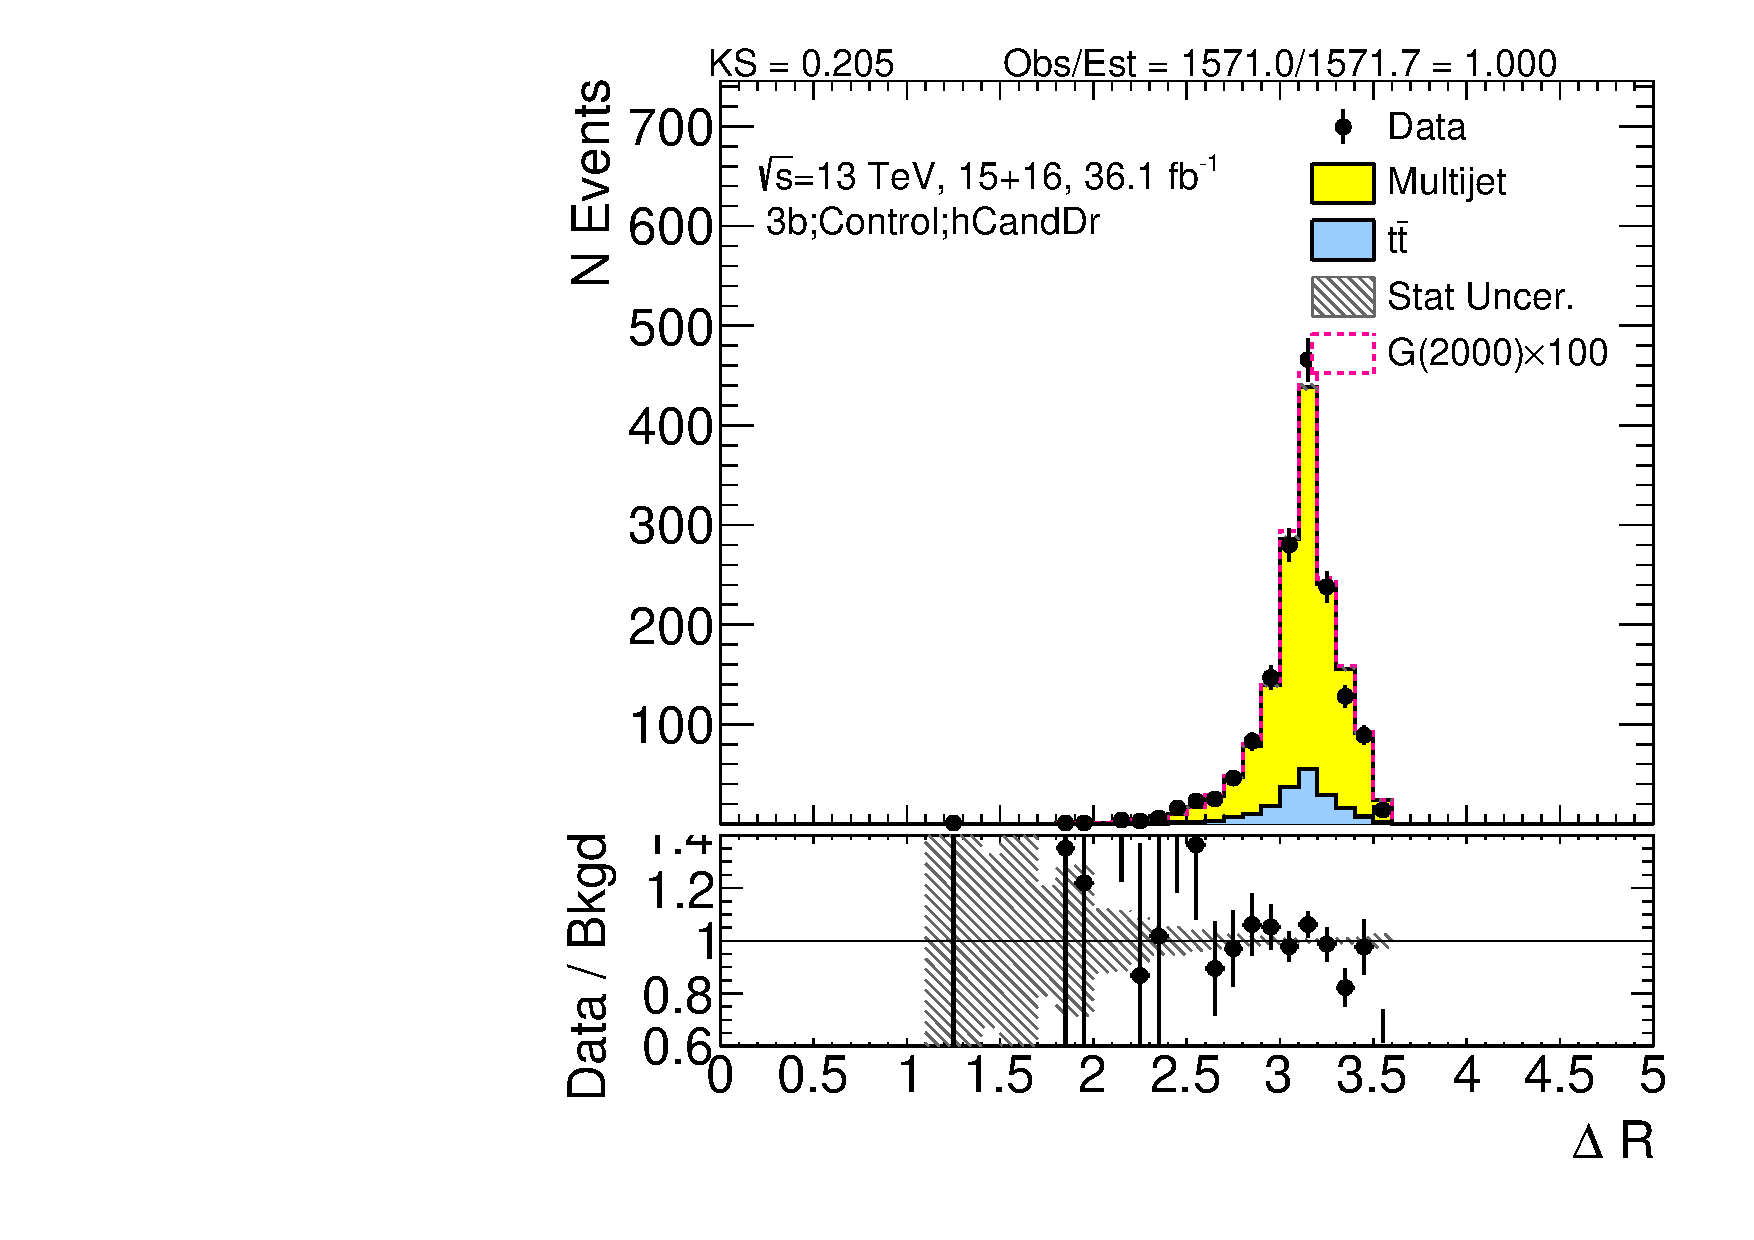
\includegraphics[width=0.33\textwidth, angle=270]{./figures/boosted/Control/Moriond_ThreeTag_Control_hCandDr.pdf}\\
0.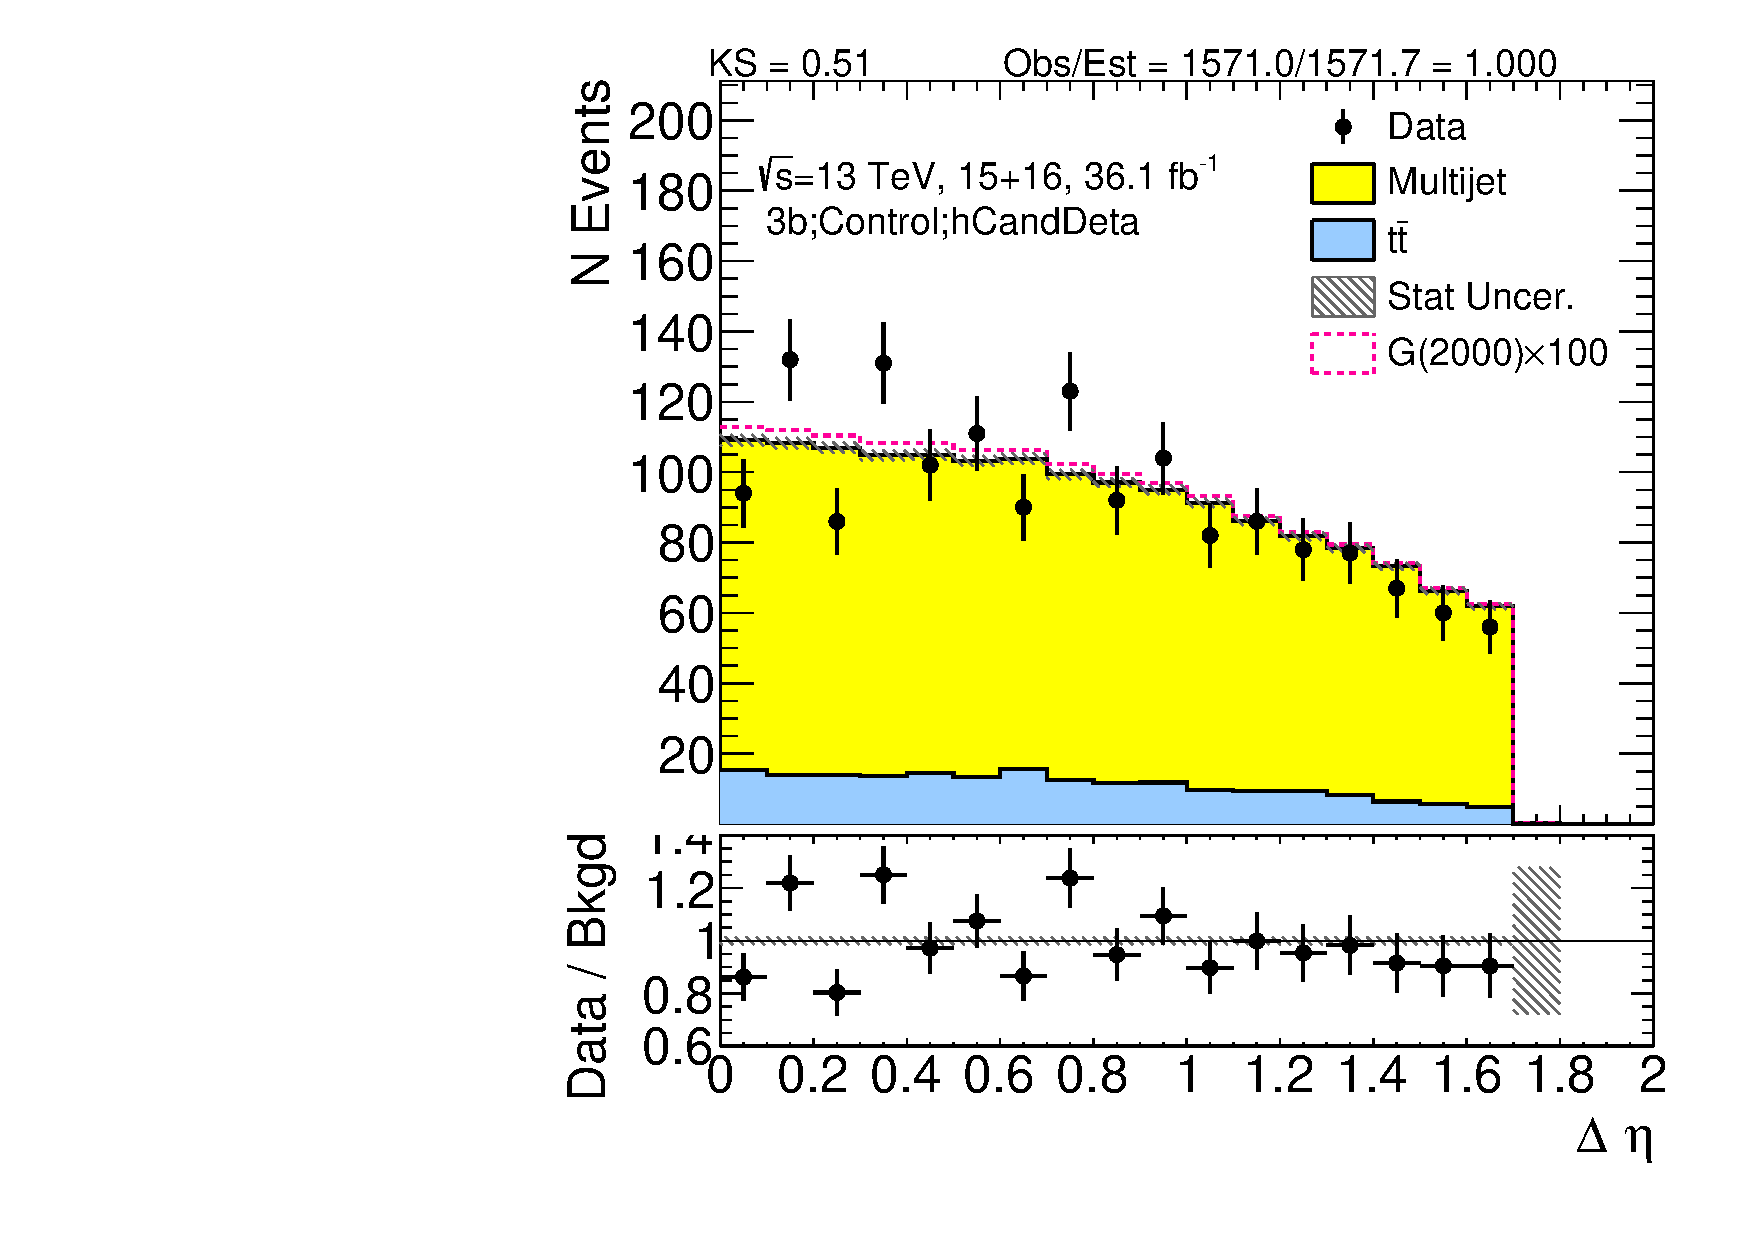
\includegraphics[width=0.33\textwidth, angle=270]{./figures/boosted/Control/Moriond_ThreeTag_Control_hCandDeta.pdf}
0.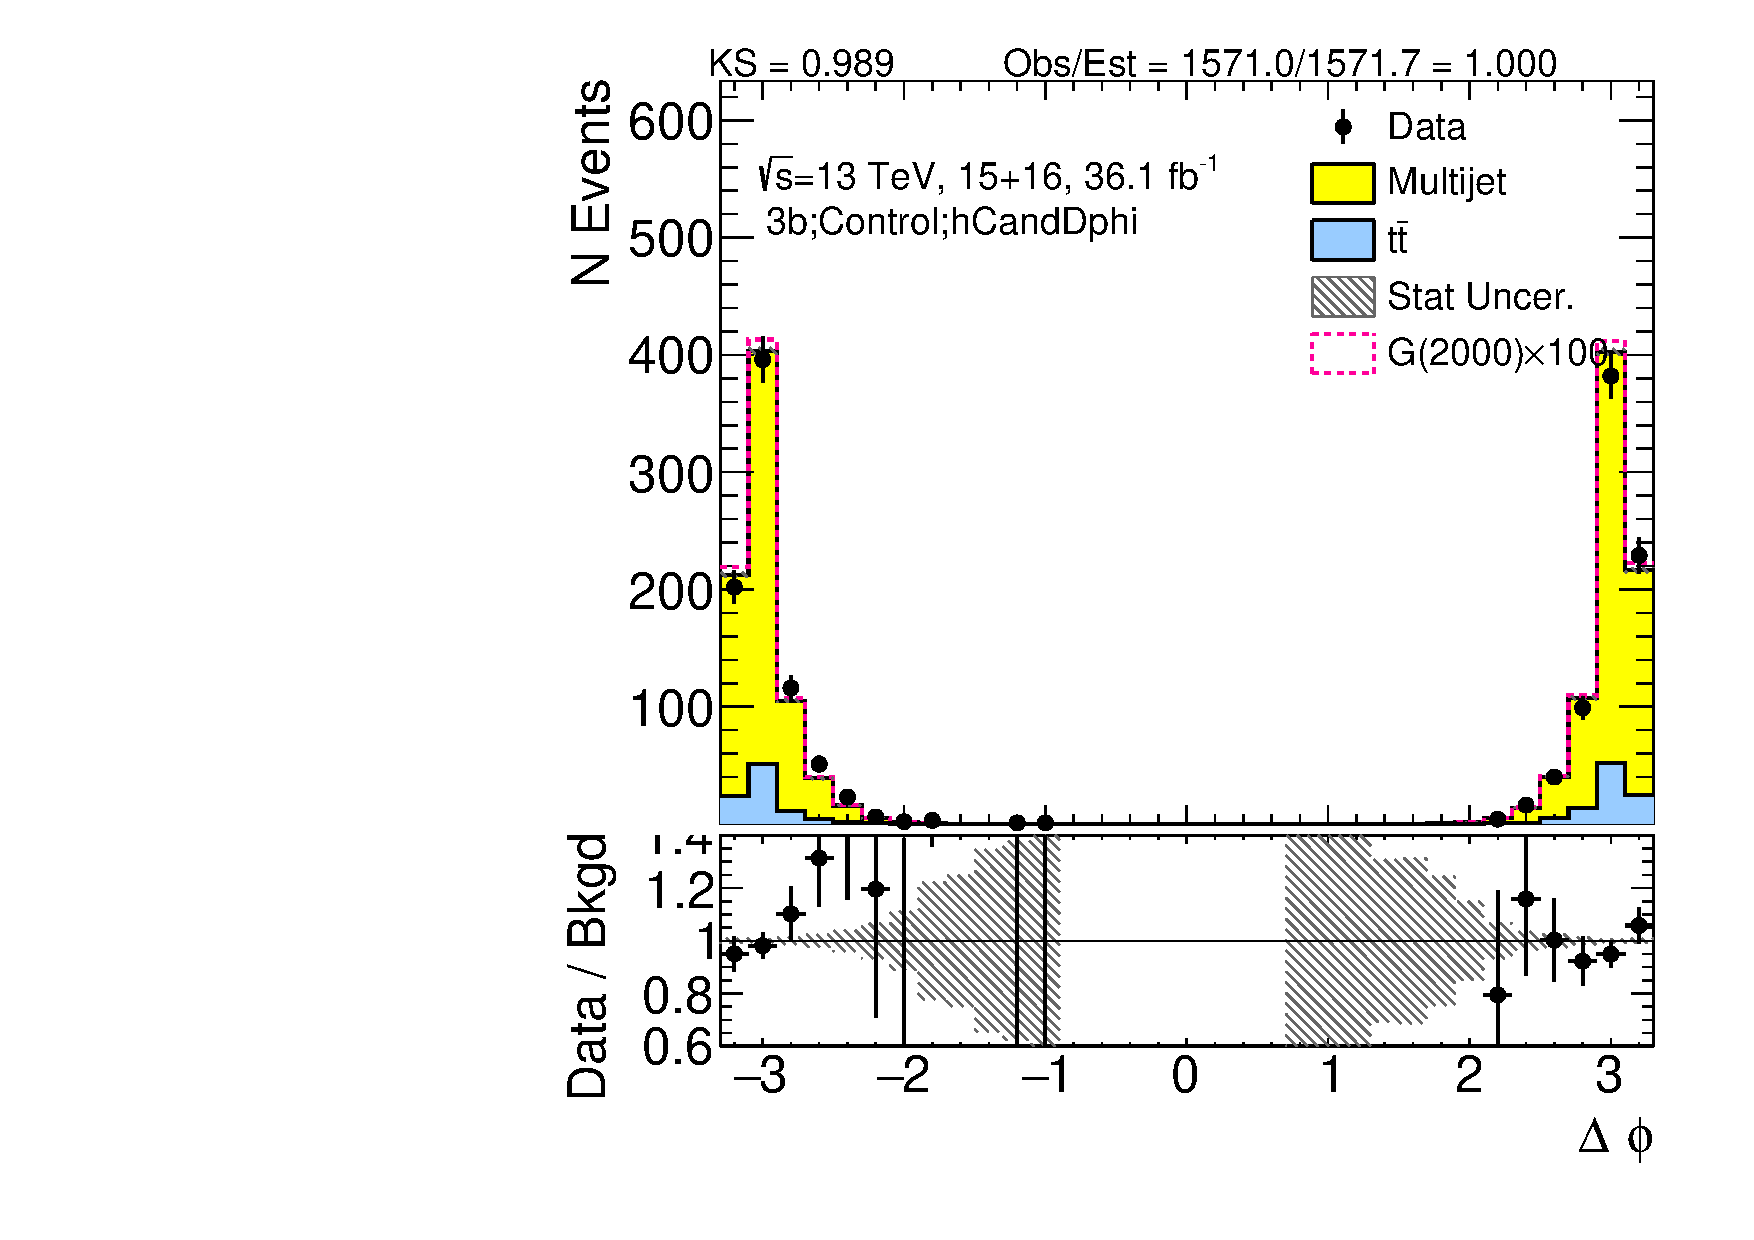
\includegraphics[width=0.33\textwidth, angle=270]{./figures/boosted/Control/Moriond_ThreeTag_Control_hCandDphi.pdf}
  \caption{Kinematics of the large-$R$ jet system in data and prediction in the sideband region after requiring 3 $b$-tags. The normalization agrees by construction, and the shapes are a feature of the prediction. }
  \label{fig:boosted-3b-control-ak10-system}
\end{center}
\end{figure*}

\clearpage

\begin{figure*}[htbp!]
\begin{center}
0.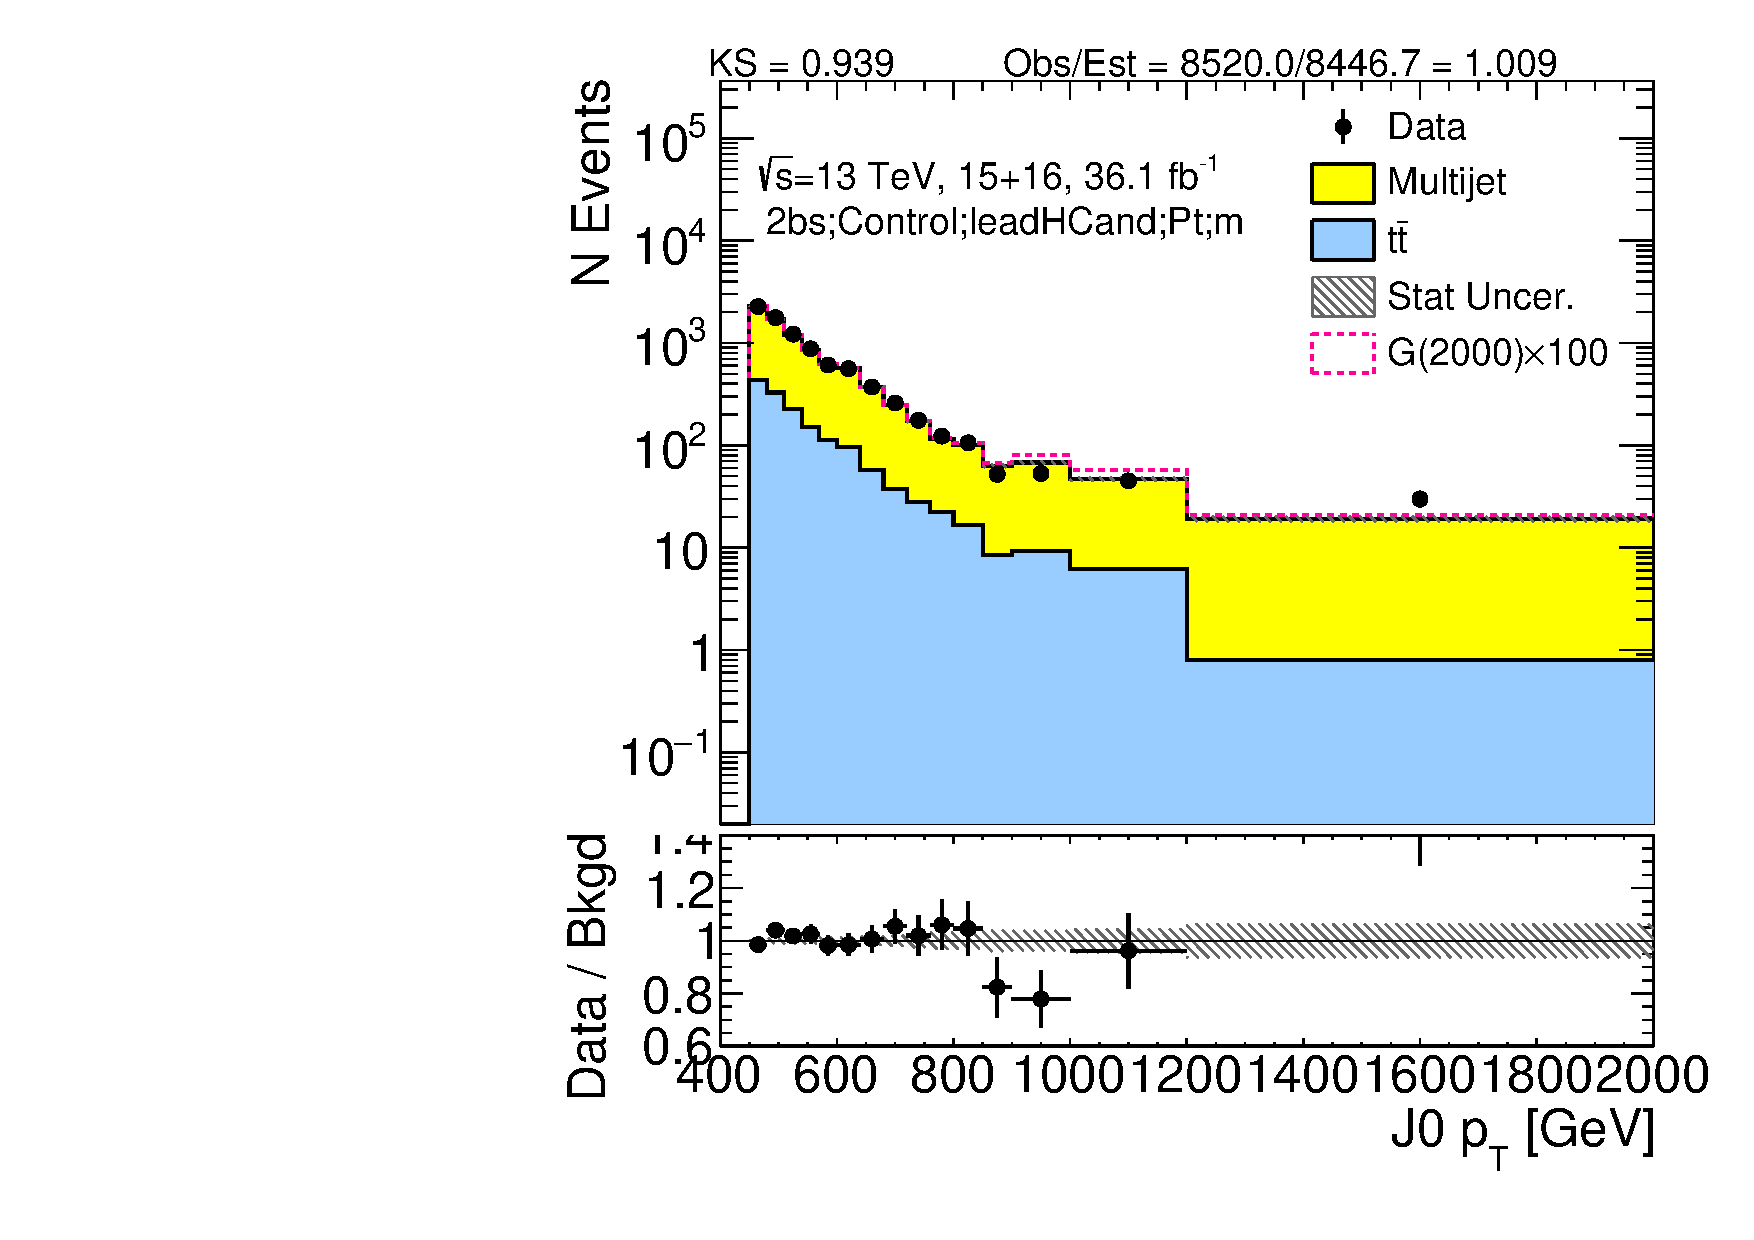
\includegraphics[width=0.33\textwidth, angle=270]{./figures/boosted/Control/Moriond_TwoTag_split_Control_leadHCand_Pt_m_1.pdf}
0.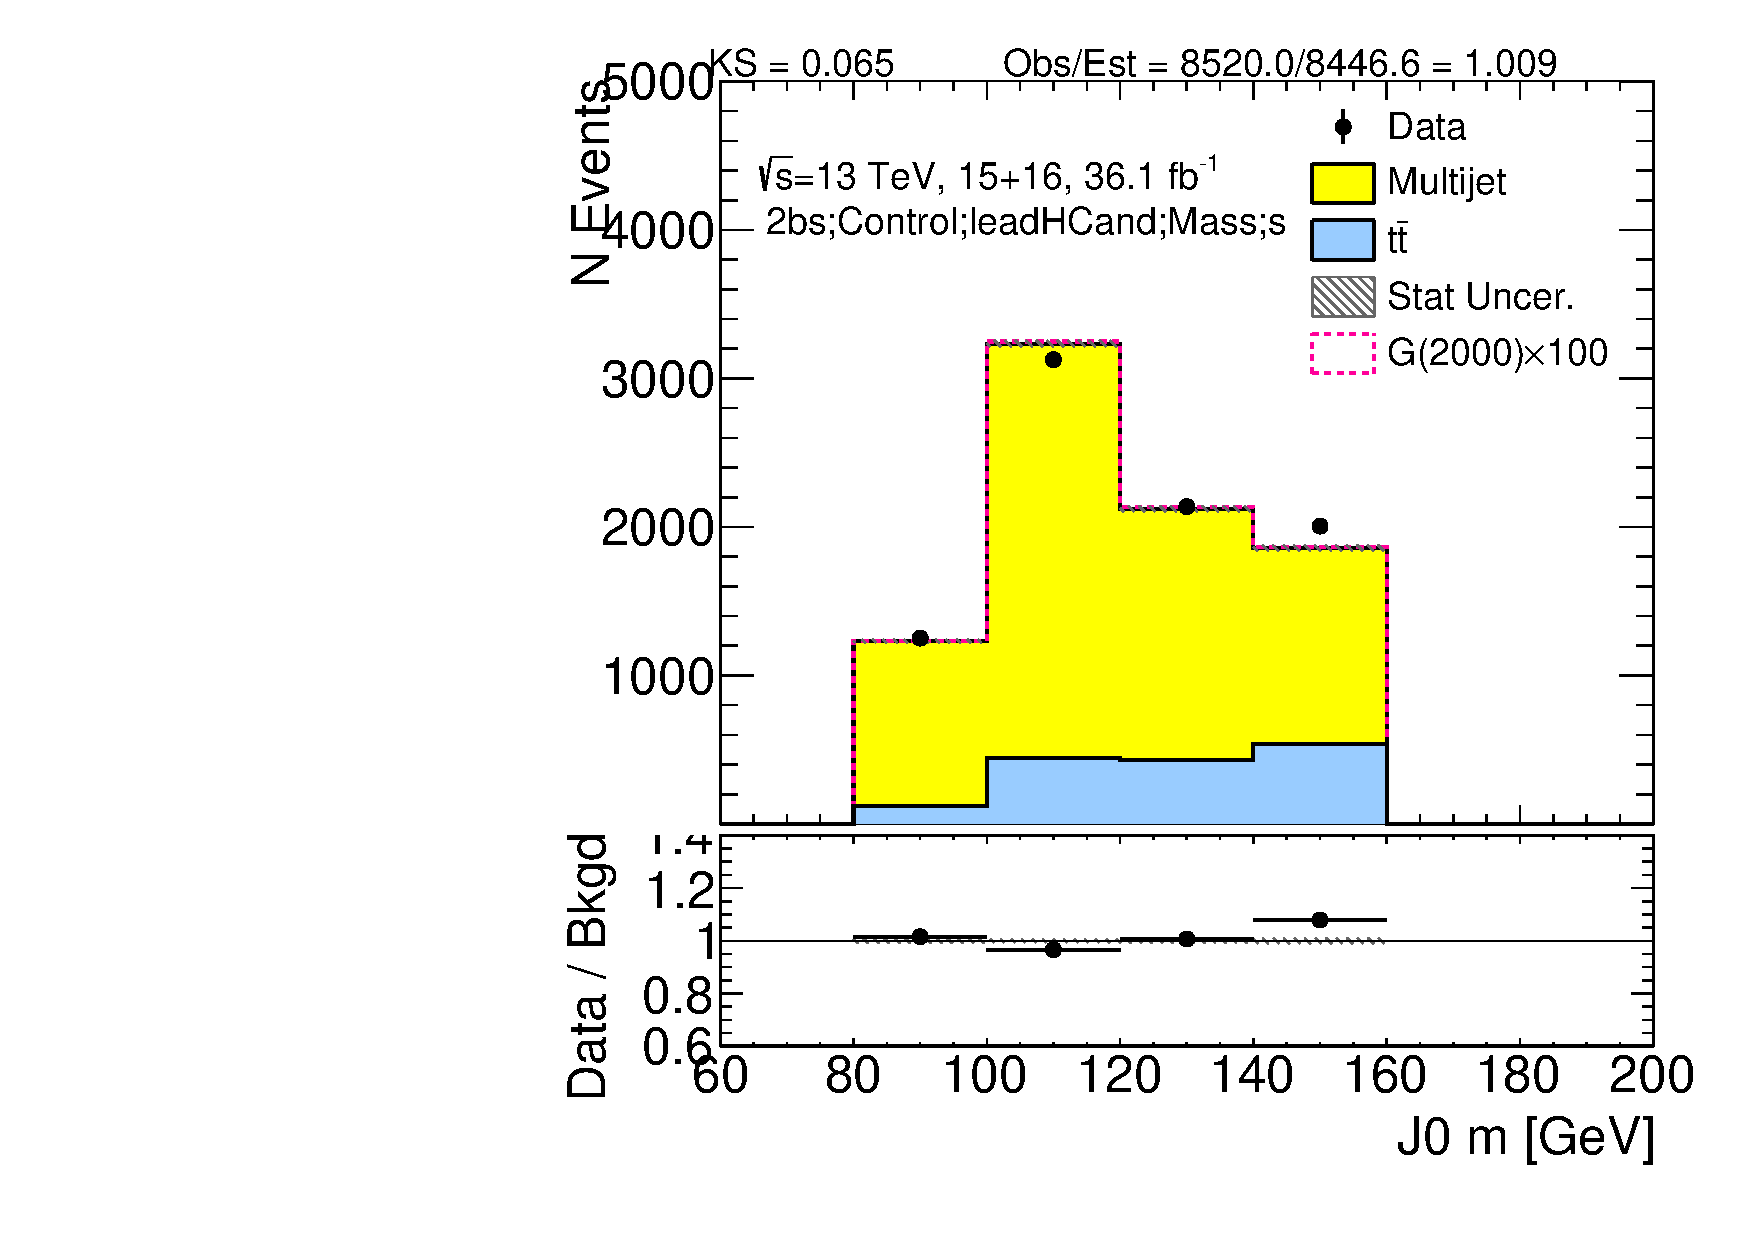
\includegraphics[width=0.33\textwidth, angle=270]{./figures/boosted/Control/Moriond_TwoTag_split_Control_leadHCand_Mass_s.pdf}\\
0.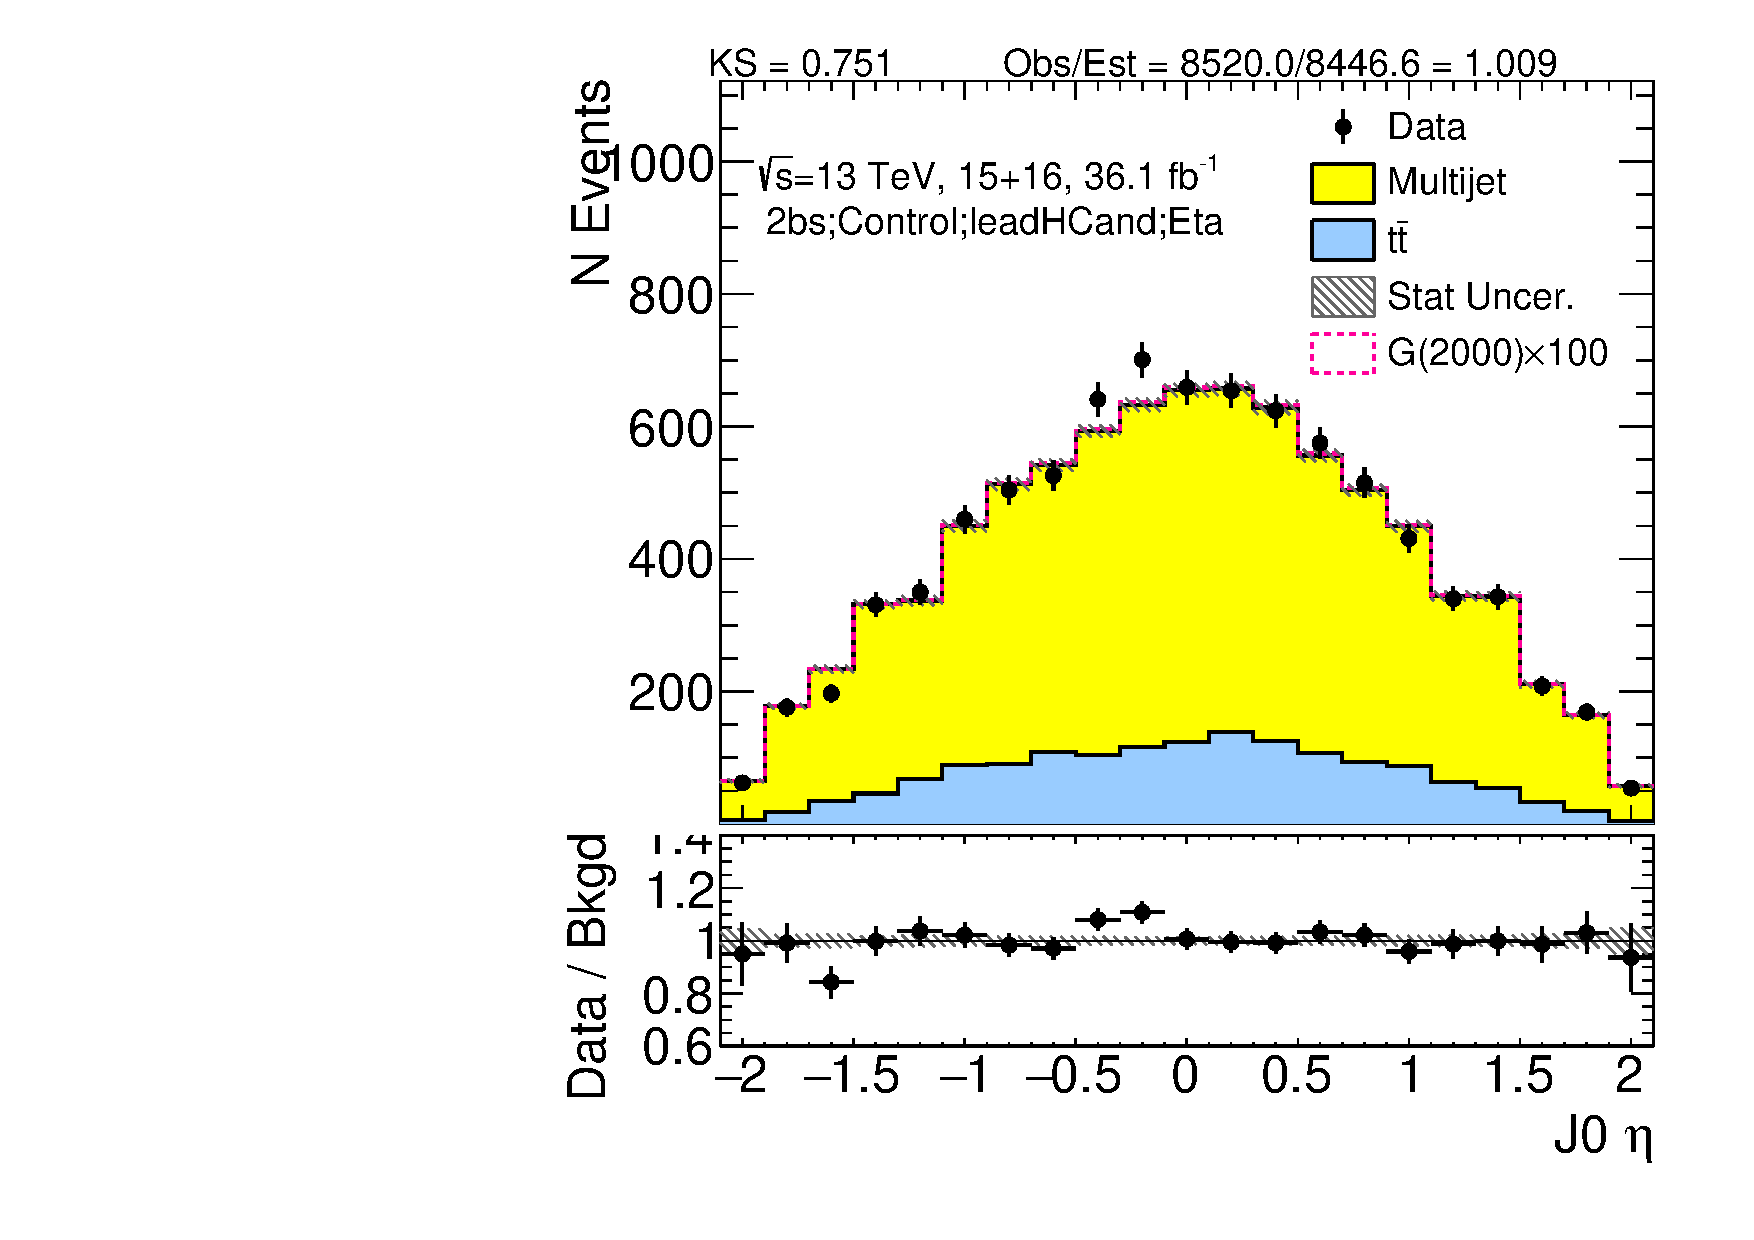
\includegraphics[width=0.33\textwidth, angle=270]{./figures/boosted/Control/Moriond_TwoTag_split_Control_leadHCand_Eta.pdf}
0.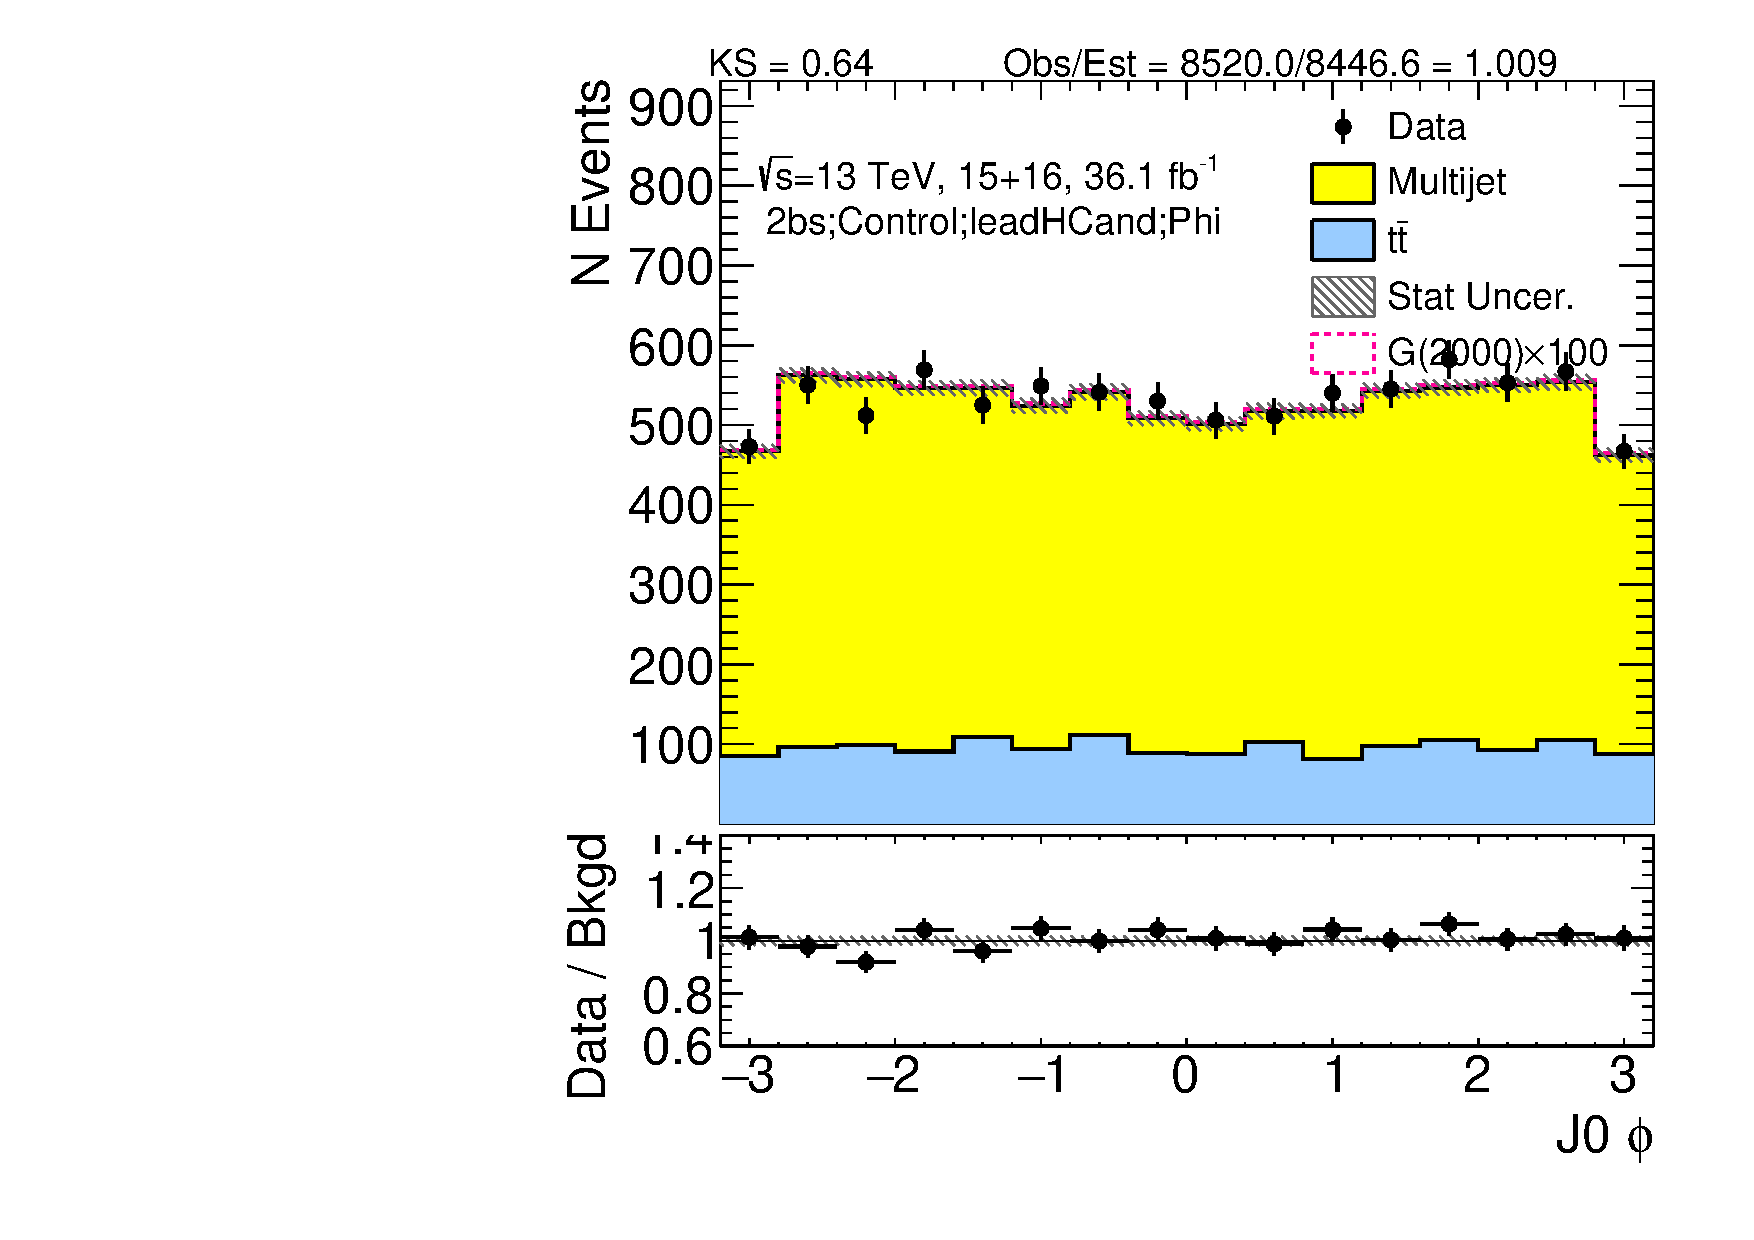
\includegraphics[width=0.33\textwidth, angle=270]{./figures/boosted/Control/Moriond_TwoTag_split_Control_leadHCand_Phi.pdf}
  \caption{Kinematics of the lead large-$R$ jet in data and prediction in the sideband region after requiring 2 $b$-tags split. The normalization agrees by construction, and the shapes are a feature of the prediction.}
  \label{fig:boosted-2bs-control-ak10-lead}
\end{center}
\end{figure*}

\begin{figure*}[htbp!]
\begin{center}
0.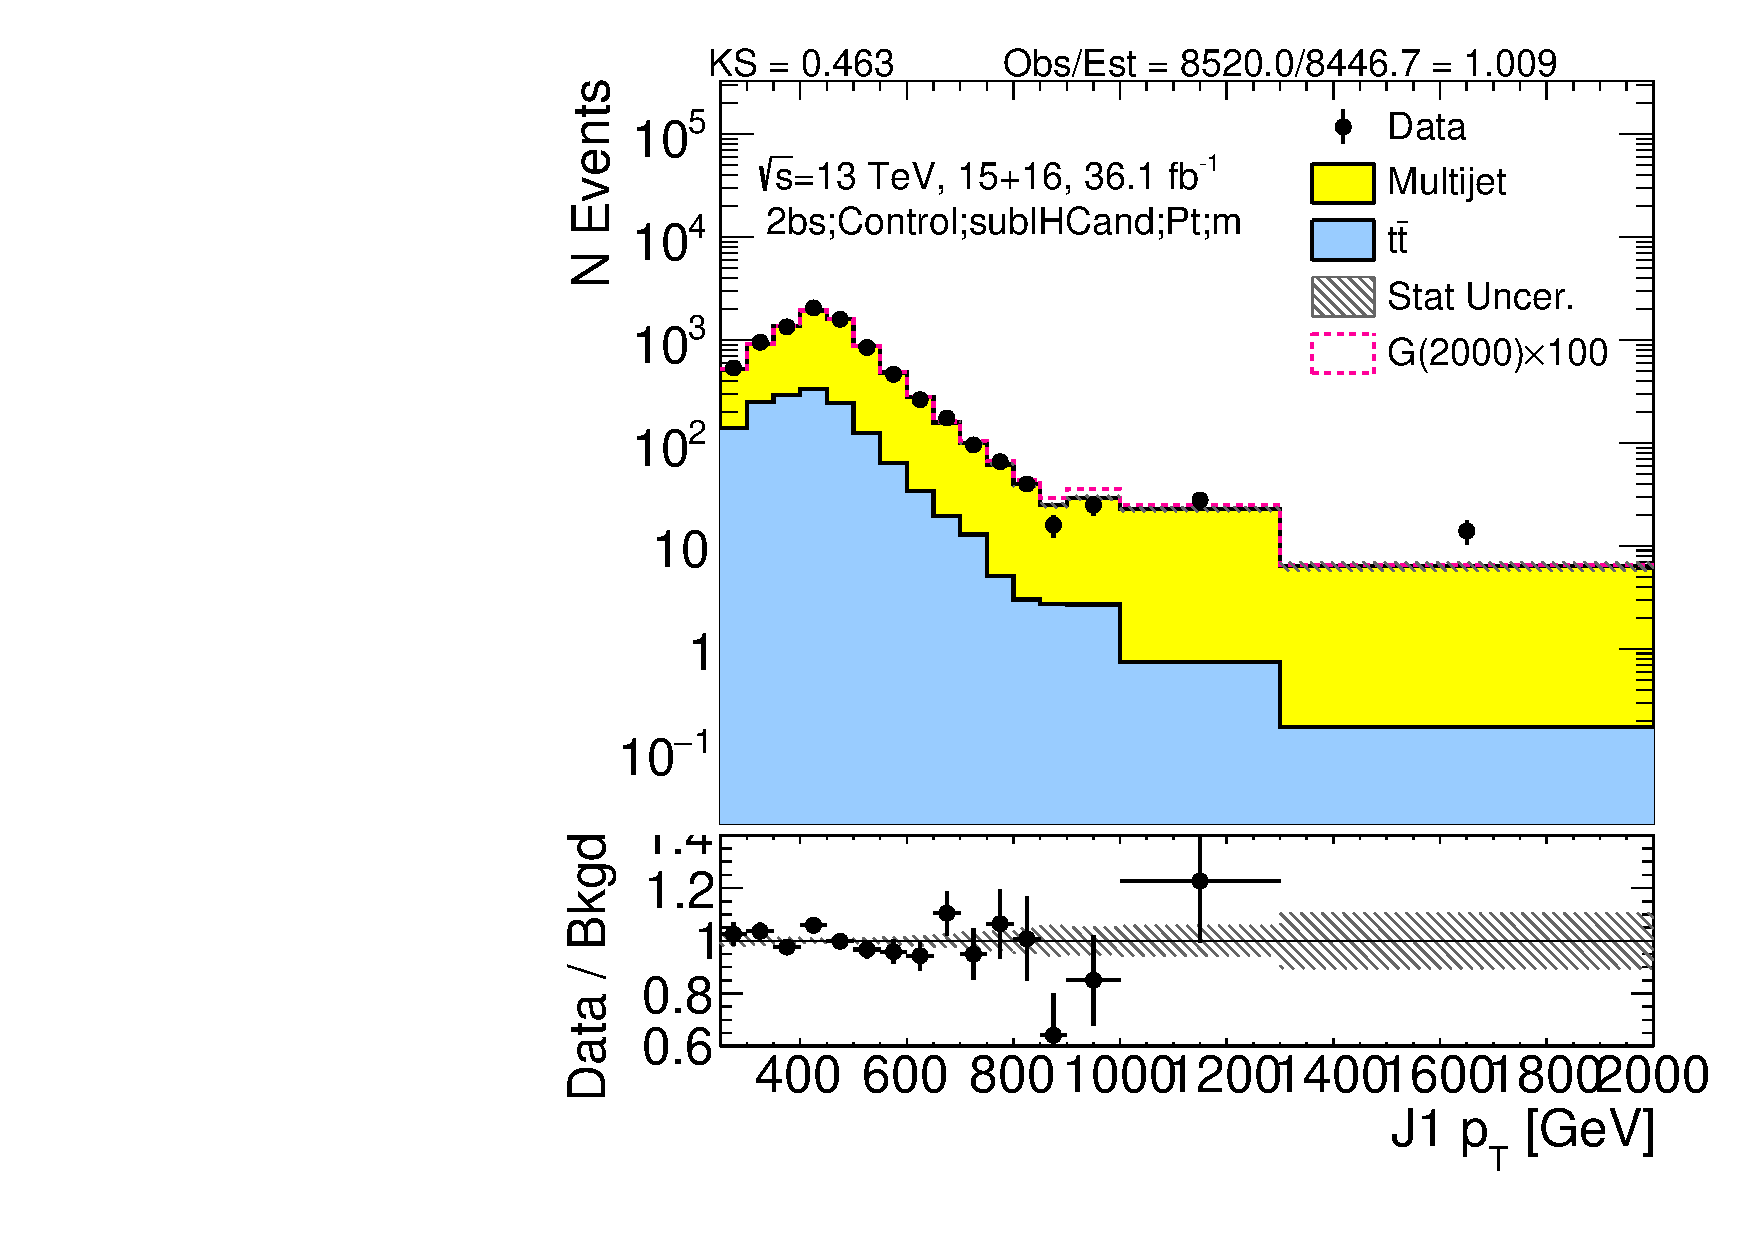
\includegraphics[width=0.33\textwidth, angle=270]{./figures/boosted/Control/Moriond_TwoTag_split_Control_sublHCand_Pt_m_1.pdf}
0.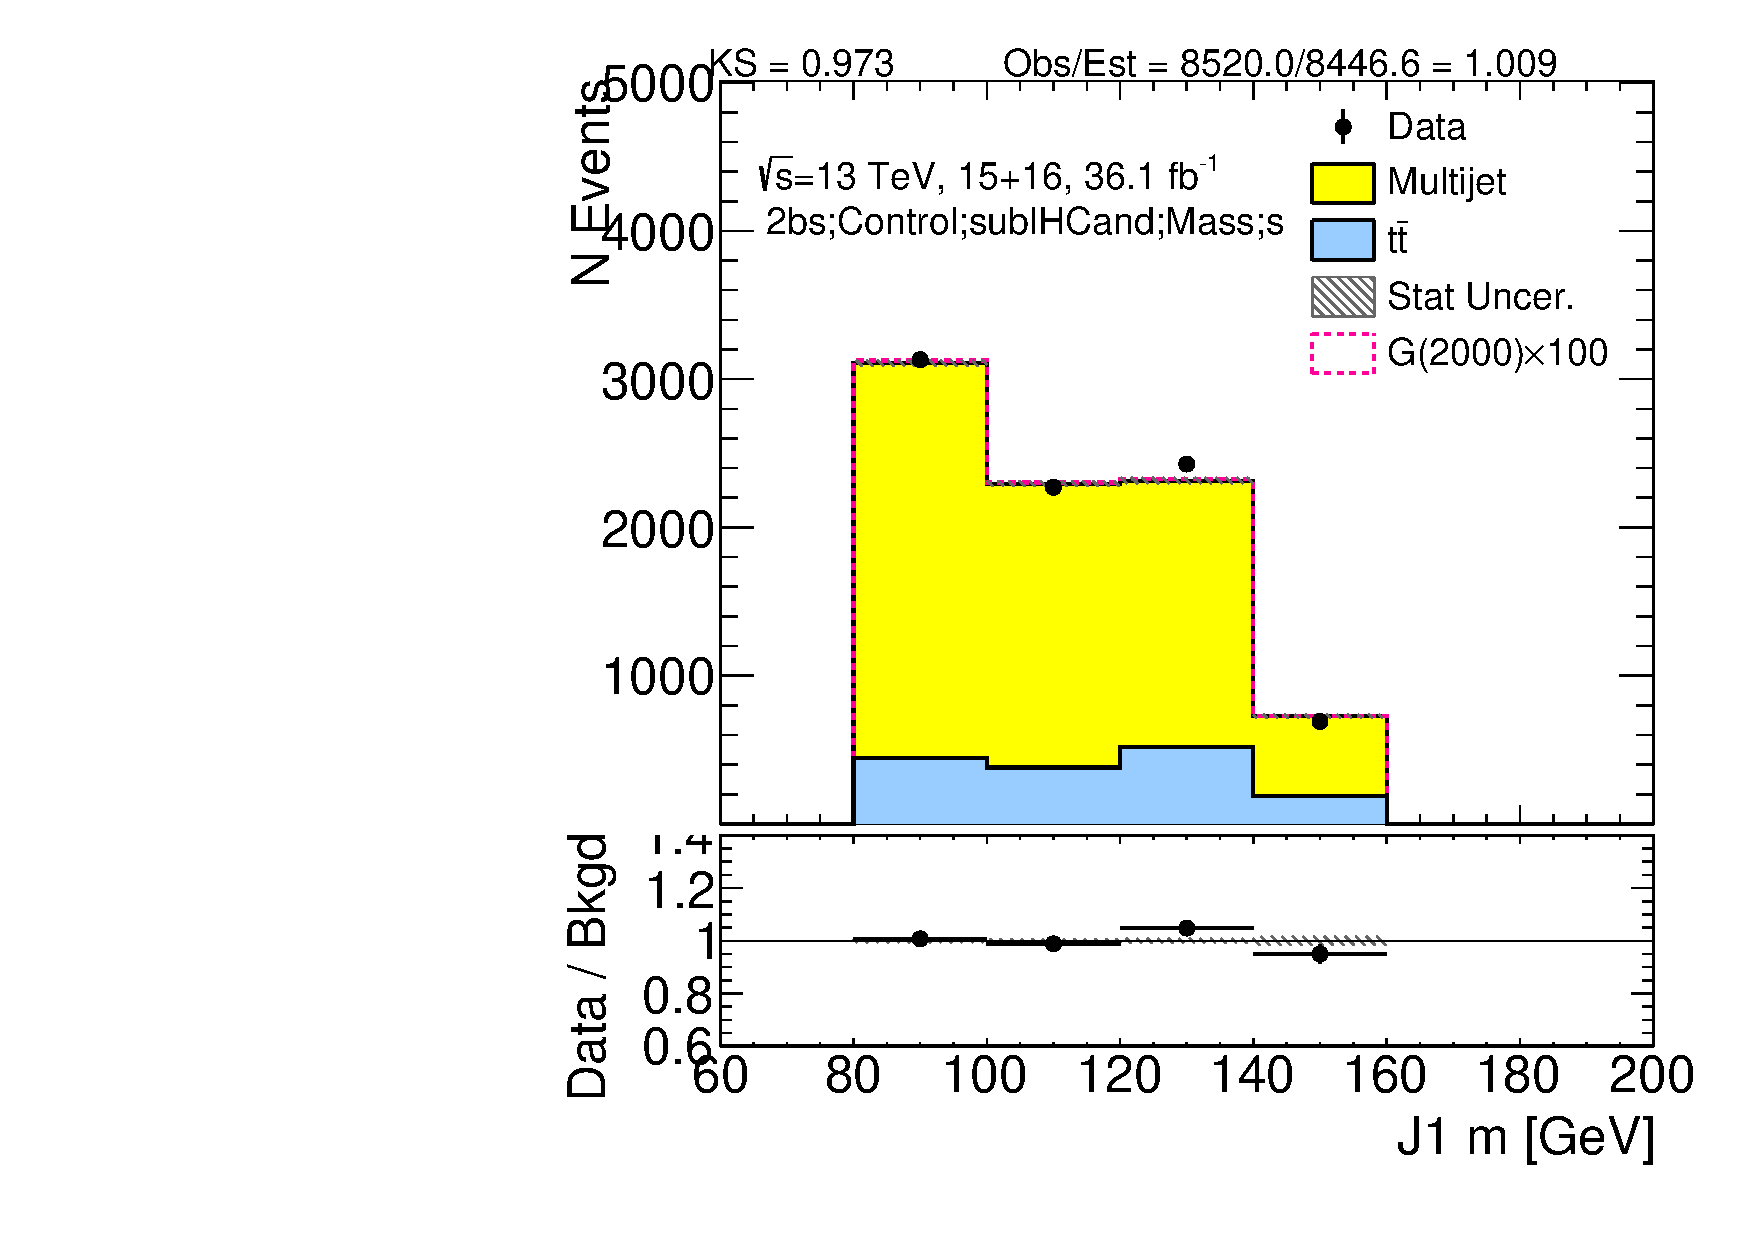
\includegraphics[width=0.33\textwidth, angle=270]{./figures/boosted/Control/Moriond_TwoTag_split_Control_sublHCand_Mass_s.pdf}\\
0.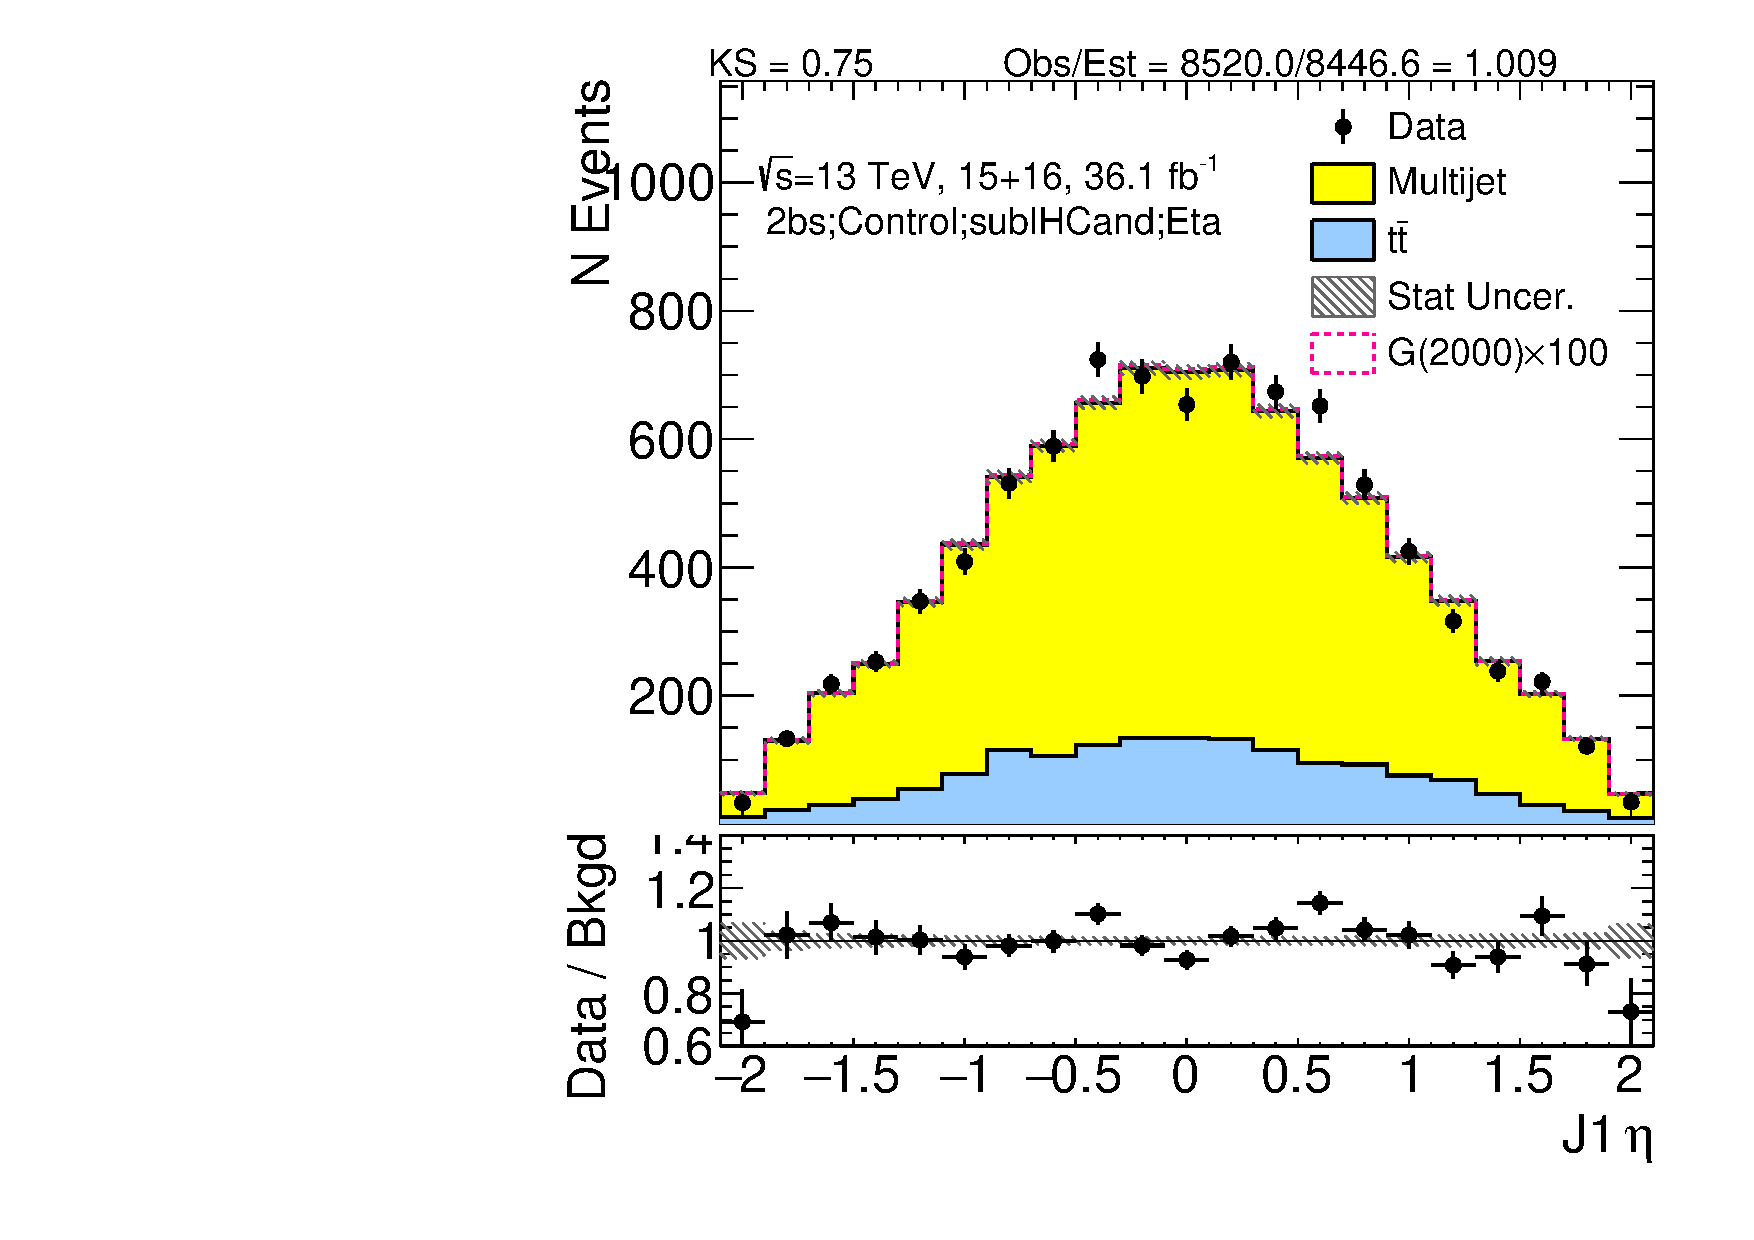
\includegraphics[width=0.33\textwidth, angle=270]{./figures/boosted/Control/Moriond_TwoTag_split_Control_sublHCand_Eta.pdf}
0.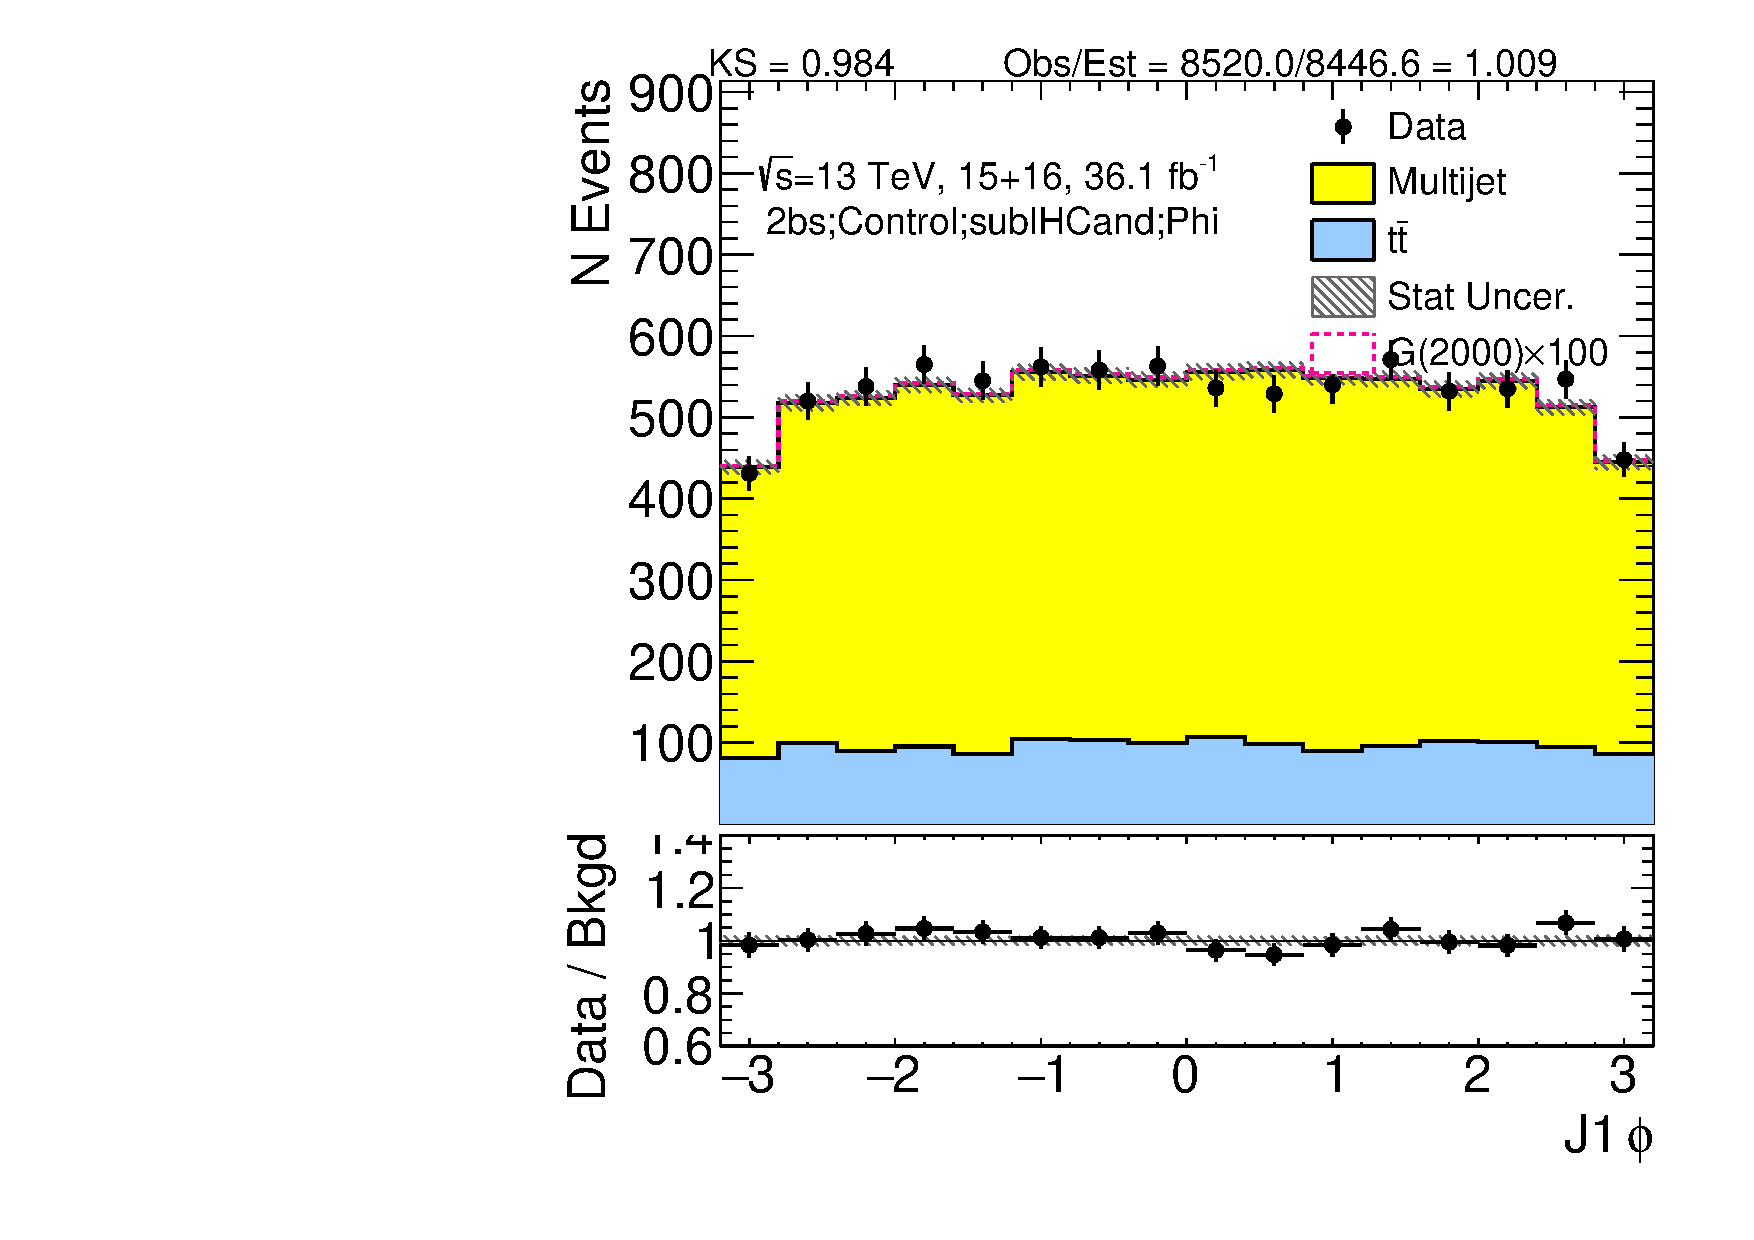
\includegraphics[width=0.33\textwidth, angle=270]{./figures/boosted/Control/Moriond_TwoTag_split_Control_sublHCand_Phi.pdf}
  \caption{Kinematics of the sub-lead large-$R$ jet in data and prediction in the sideband region after requiring 2 $b$-tags split. The normalization agrees by construction, and the shapes are a feature of the prediction.}
  \label{fig:boosted-2bs-control-ak10-subl}
\end{center}
\end{figure*}

\begin{figure*}[htbp!]
\begin{center}
0.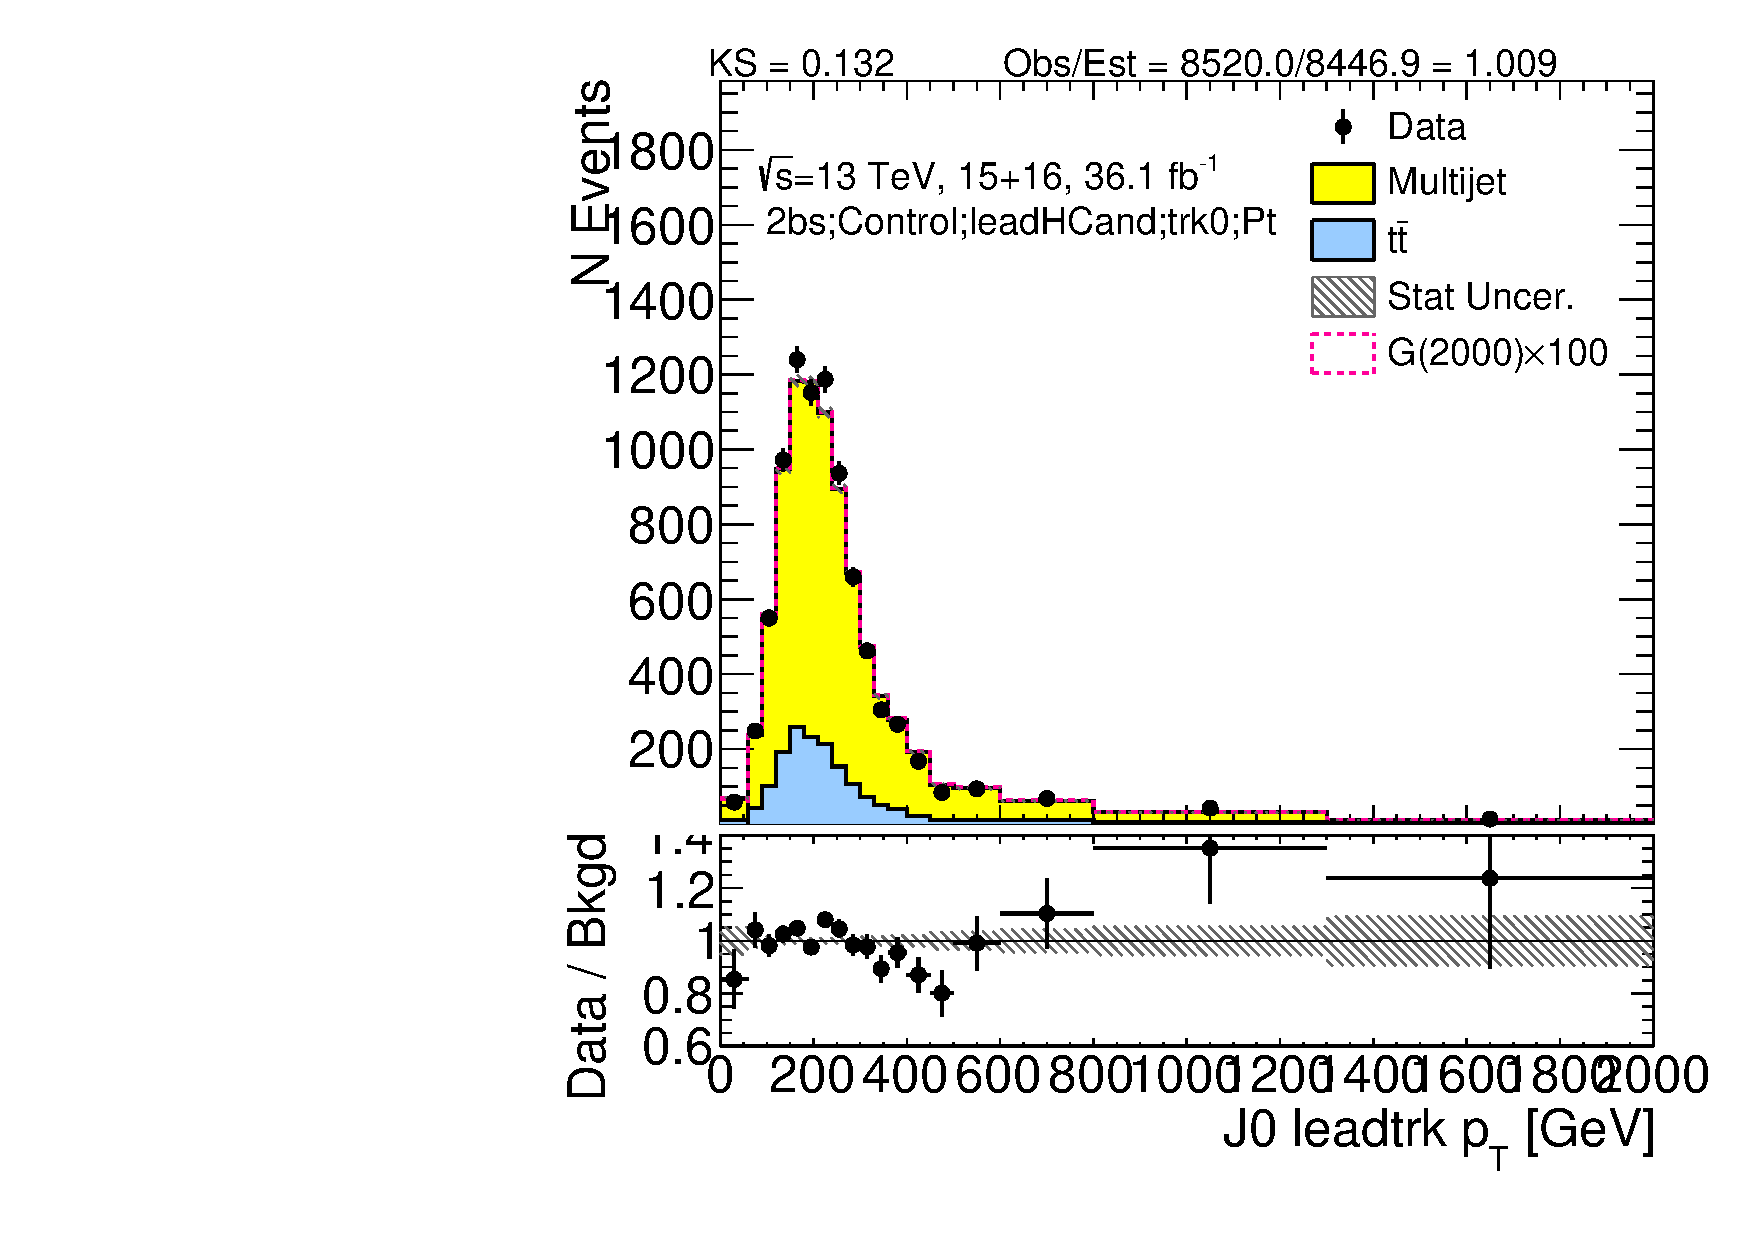
\includegraphics[width=0.33\textwidth, angle=270]{./figures/boosted/Control/Moriond_TwoTag_split_Control_leadHCand_trk0_Pt.pdf}
0.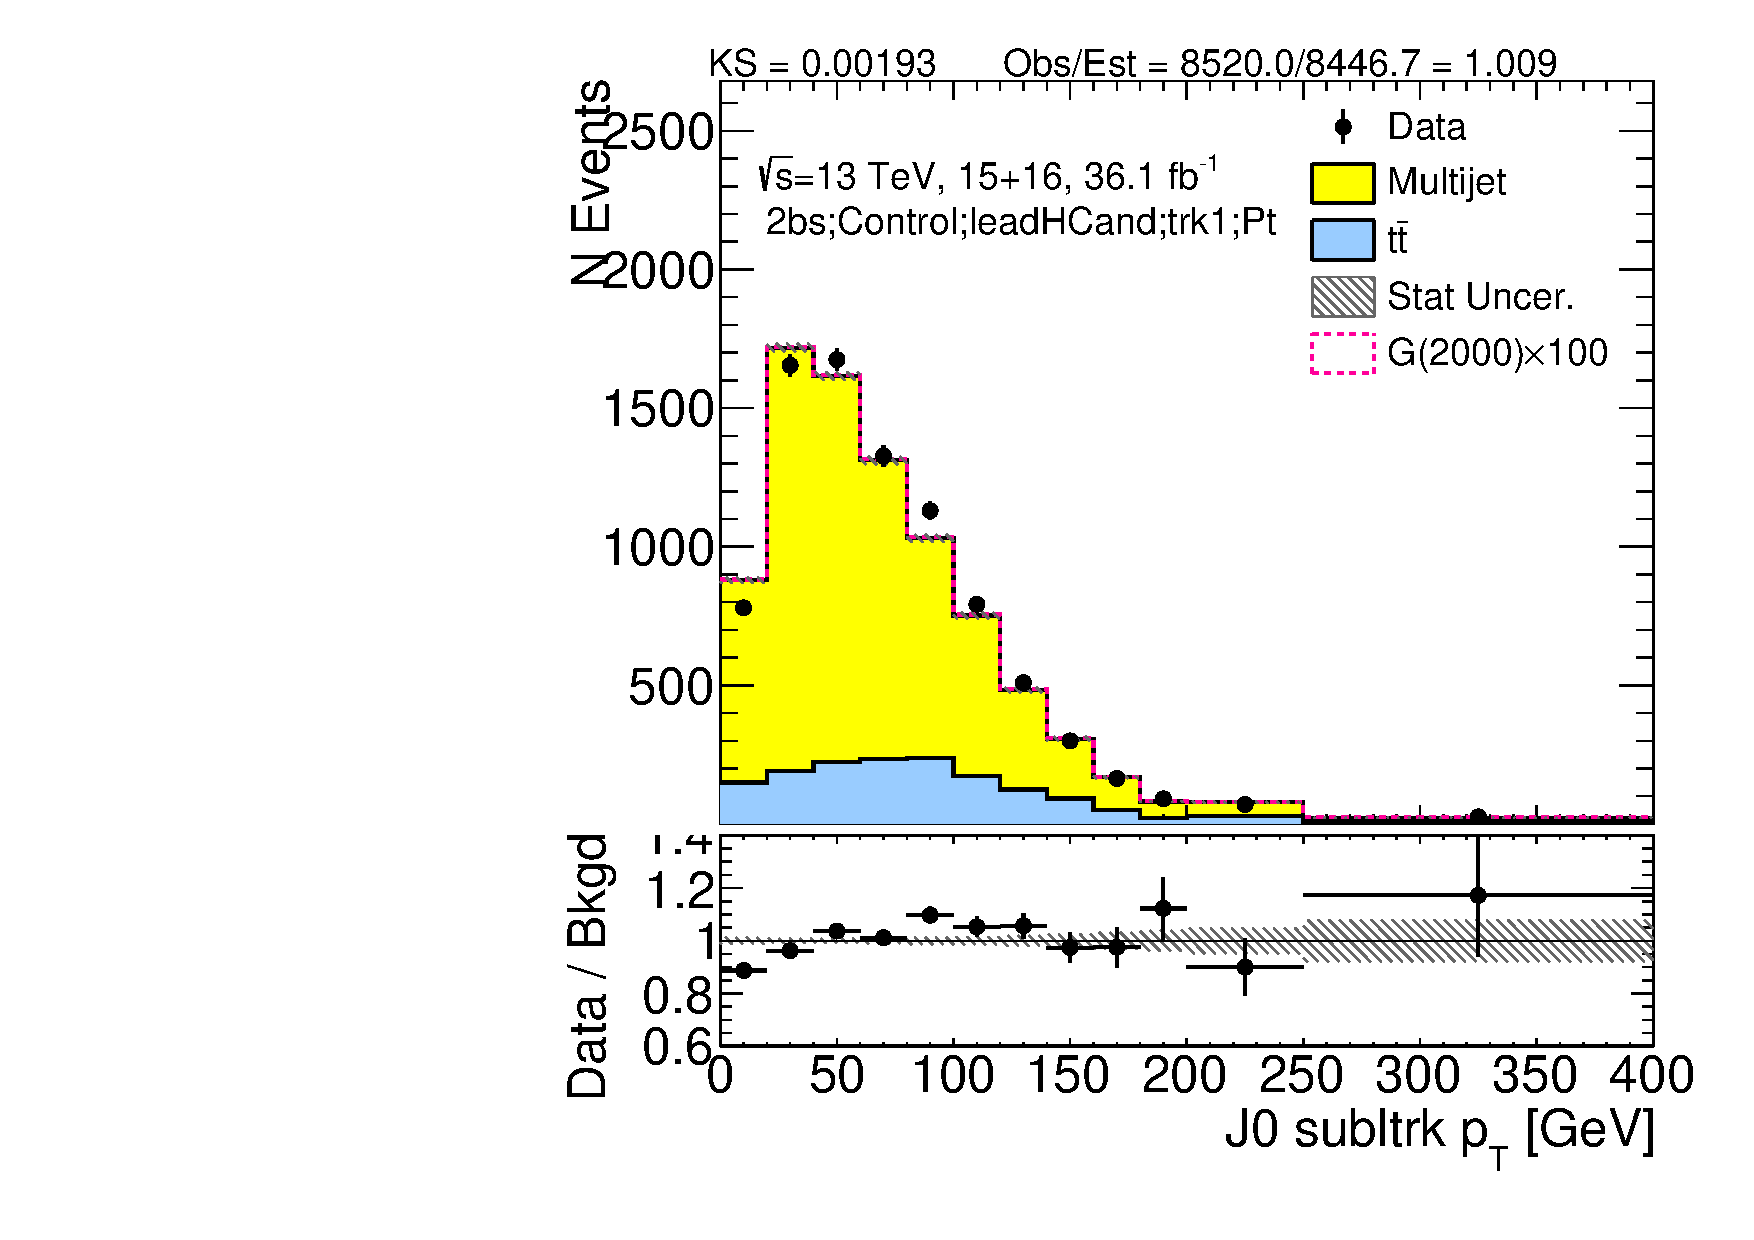
\includegraphics[width=0.33\textwidth, angle=270]{./figures/boosted/Control/Moriond_TwoTag_split_Control_leadHCand_trk1_Pt.pdf}\\
0.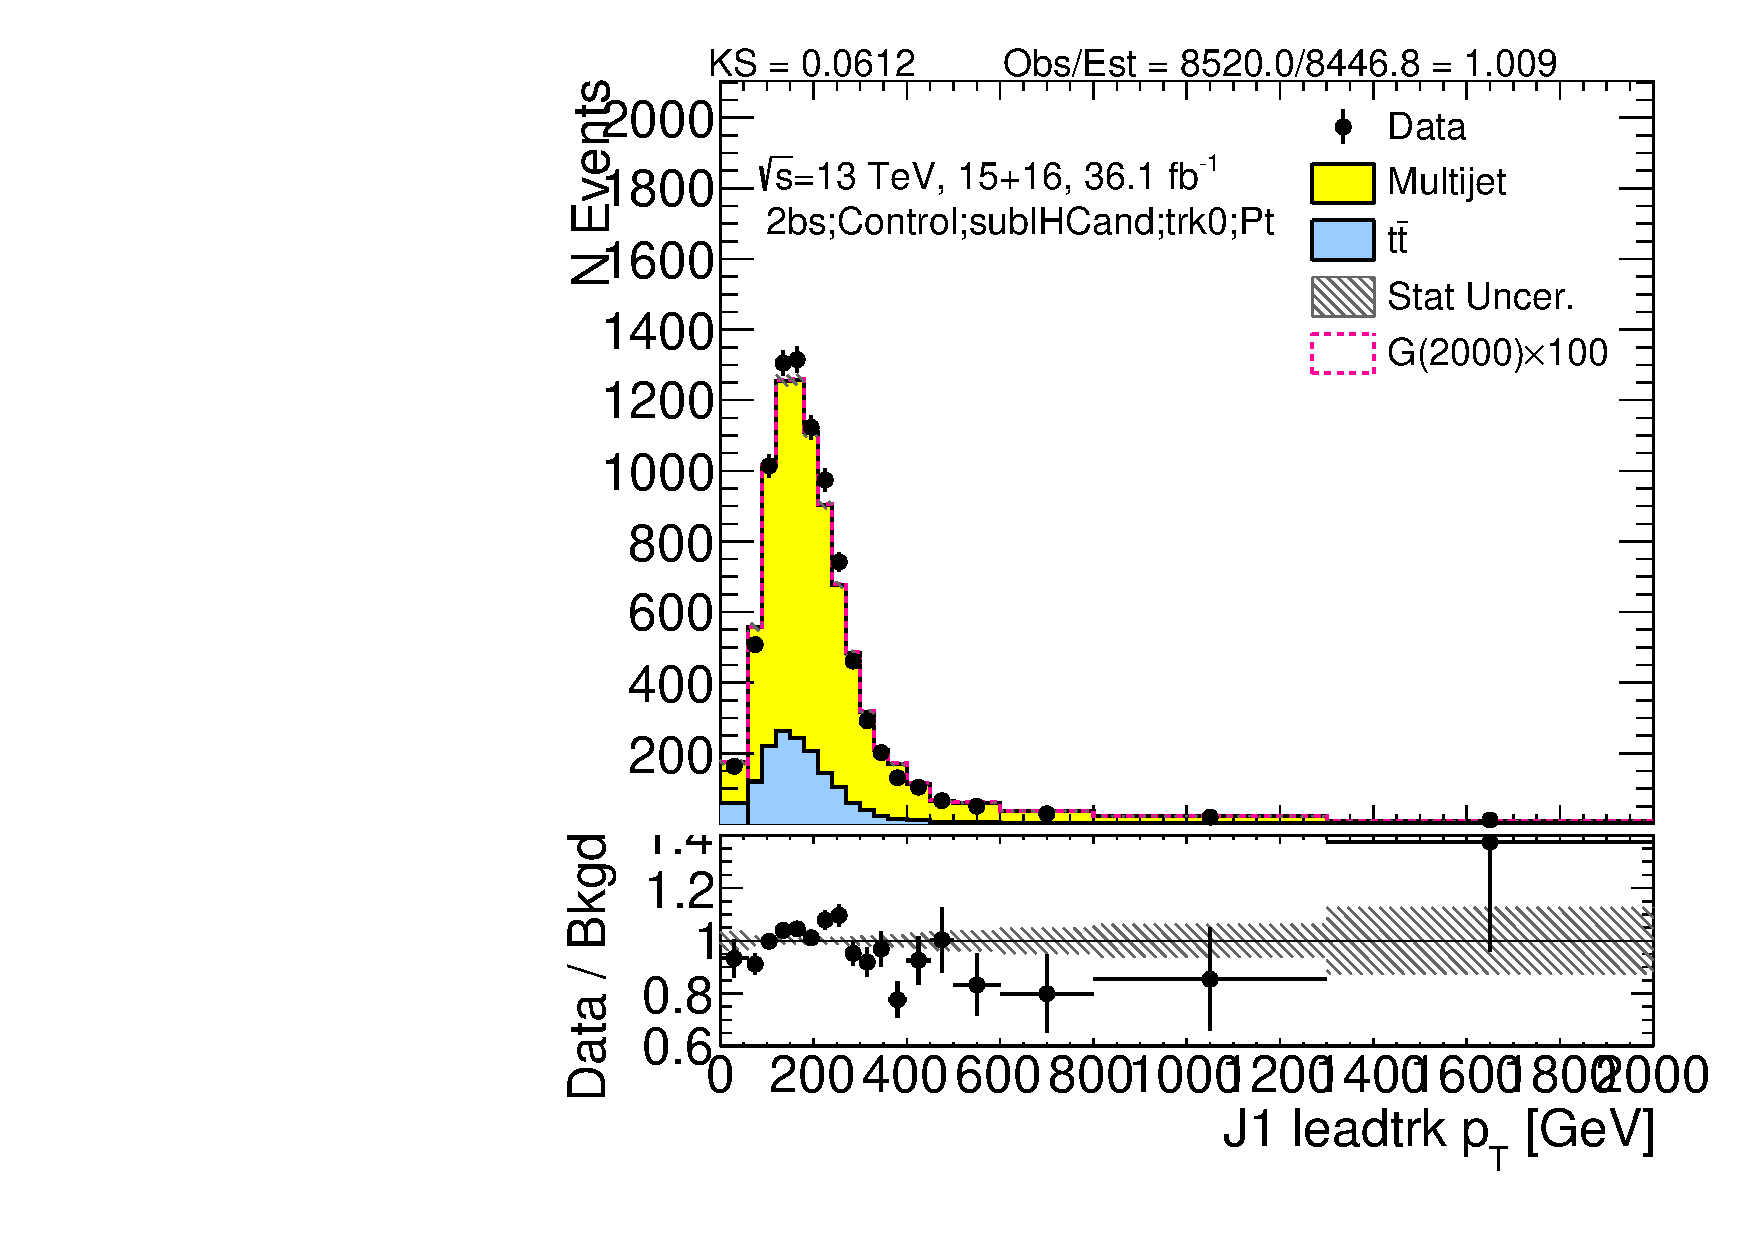
\includegraphics[width=0.33\textwidth, angle=270]{./figures/boosted/Control/Moriond_TwoTag_split_Control_sublHCand_trk0_Pt.pdf}
0.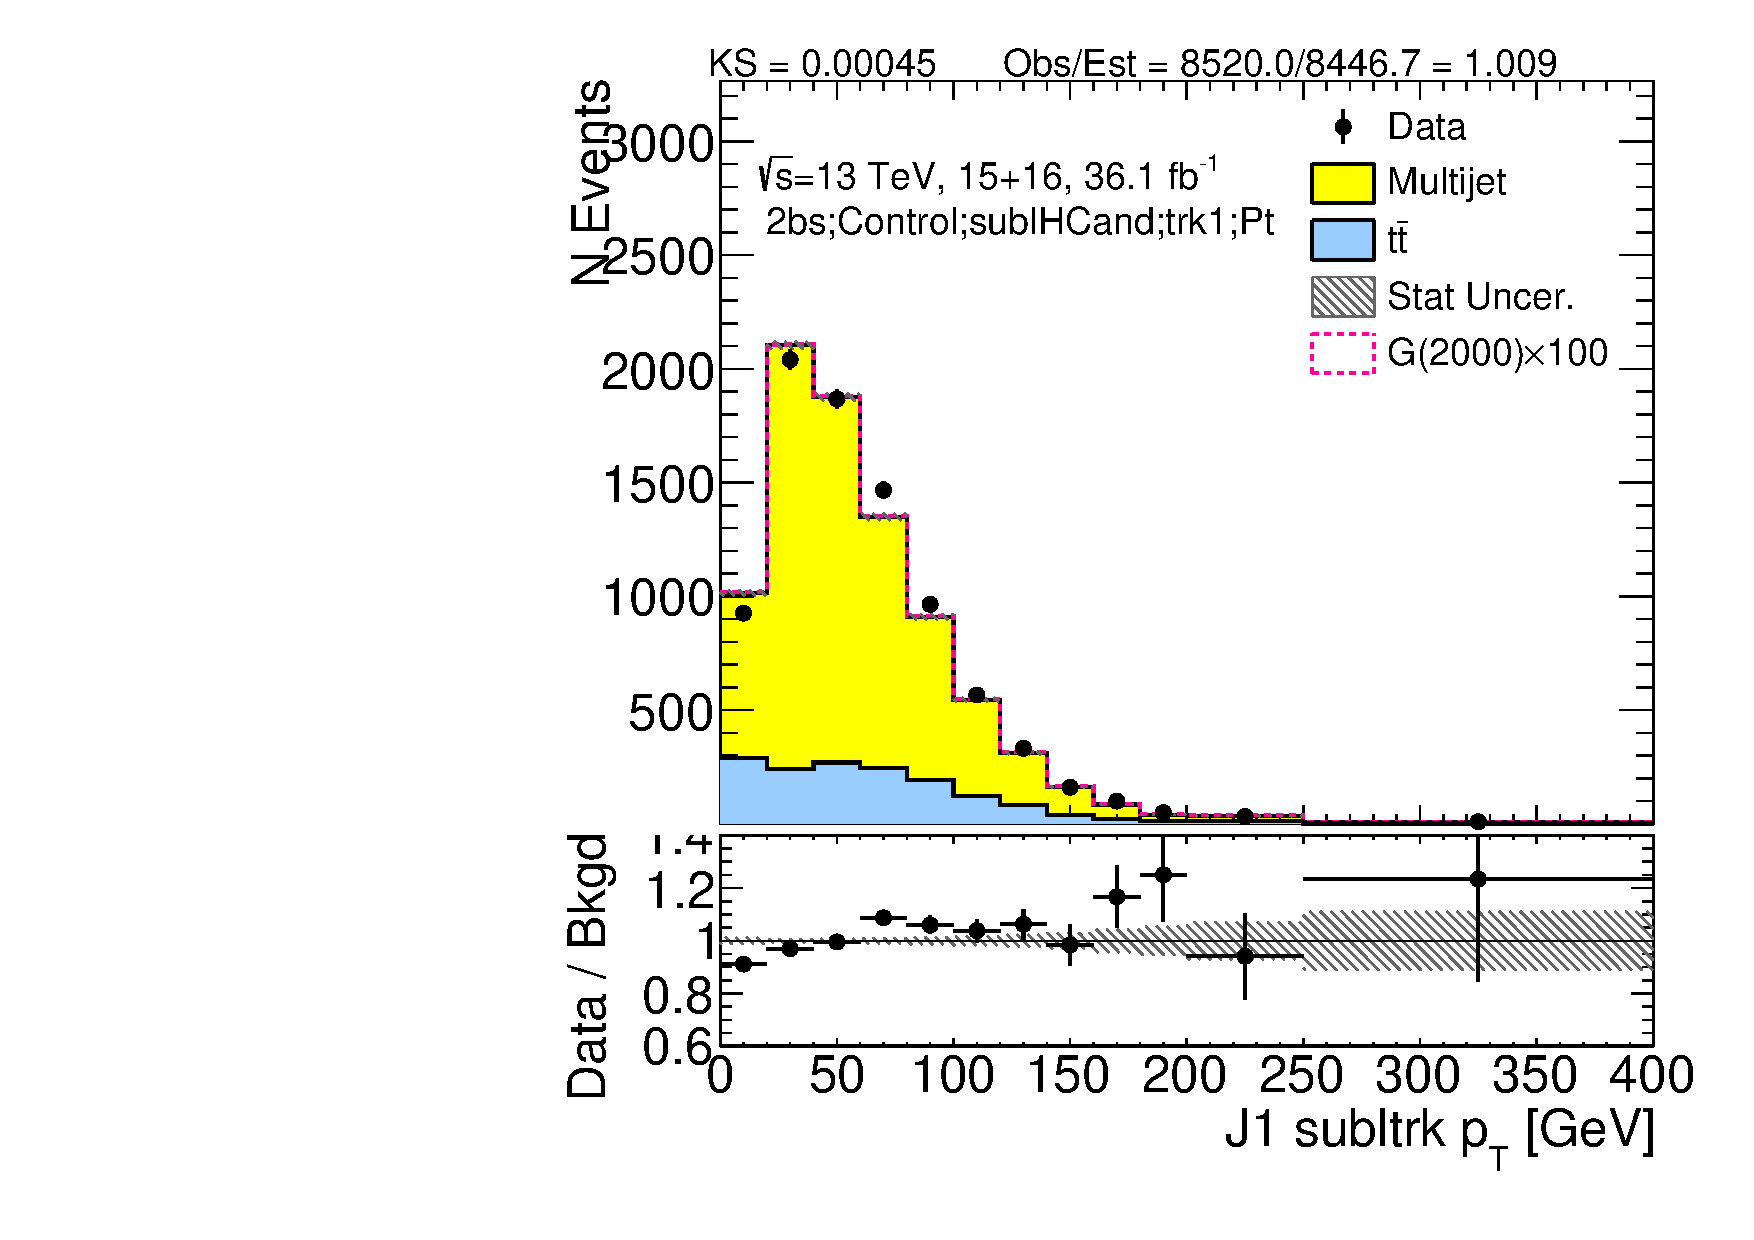
\includegraphics[width=0.33\textwidth, angle=270]{./figures/boosted/Control/Moriond_TwoTag_split_Control_sublHCand_trk1_Pt.pdf}\\
0.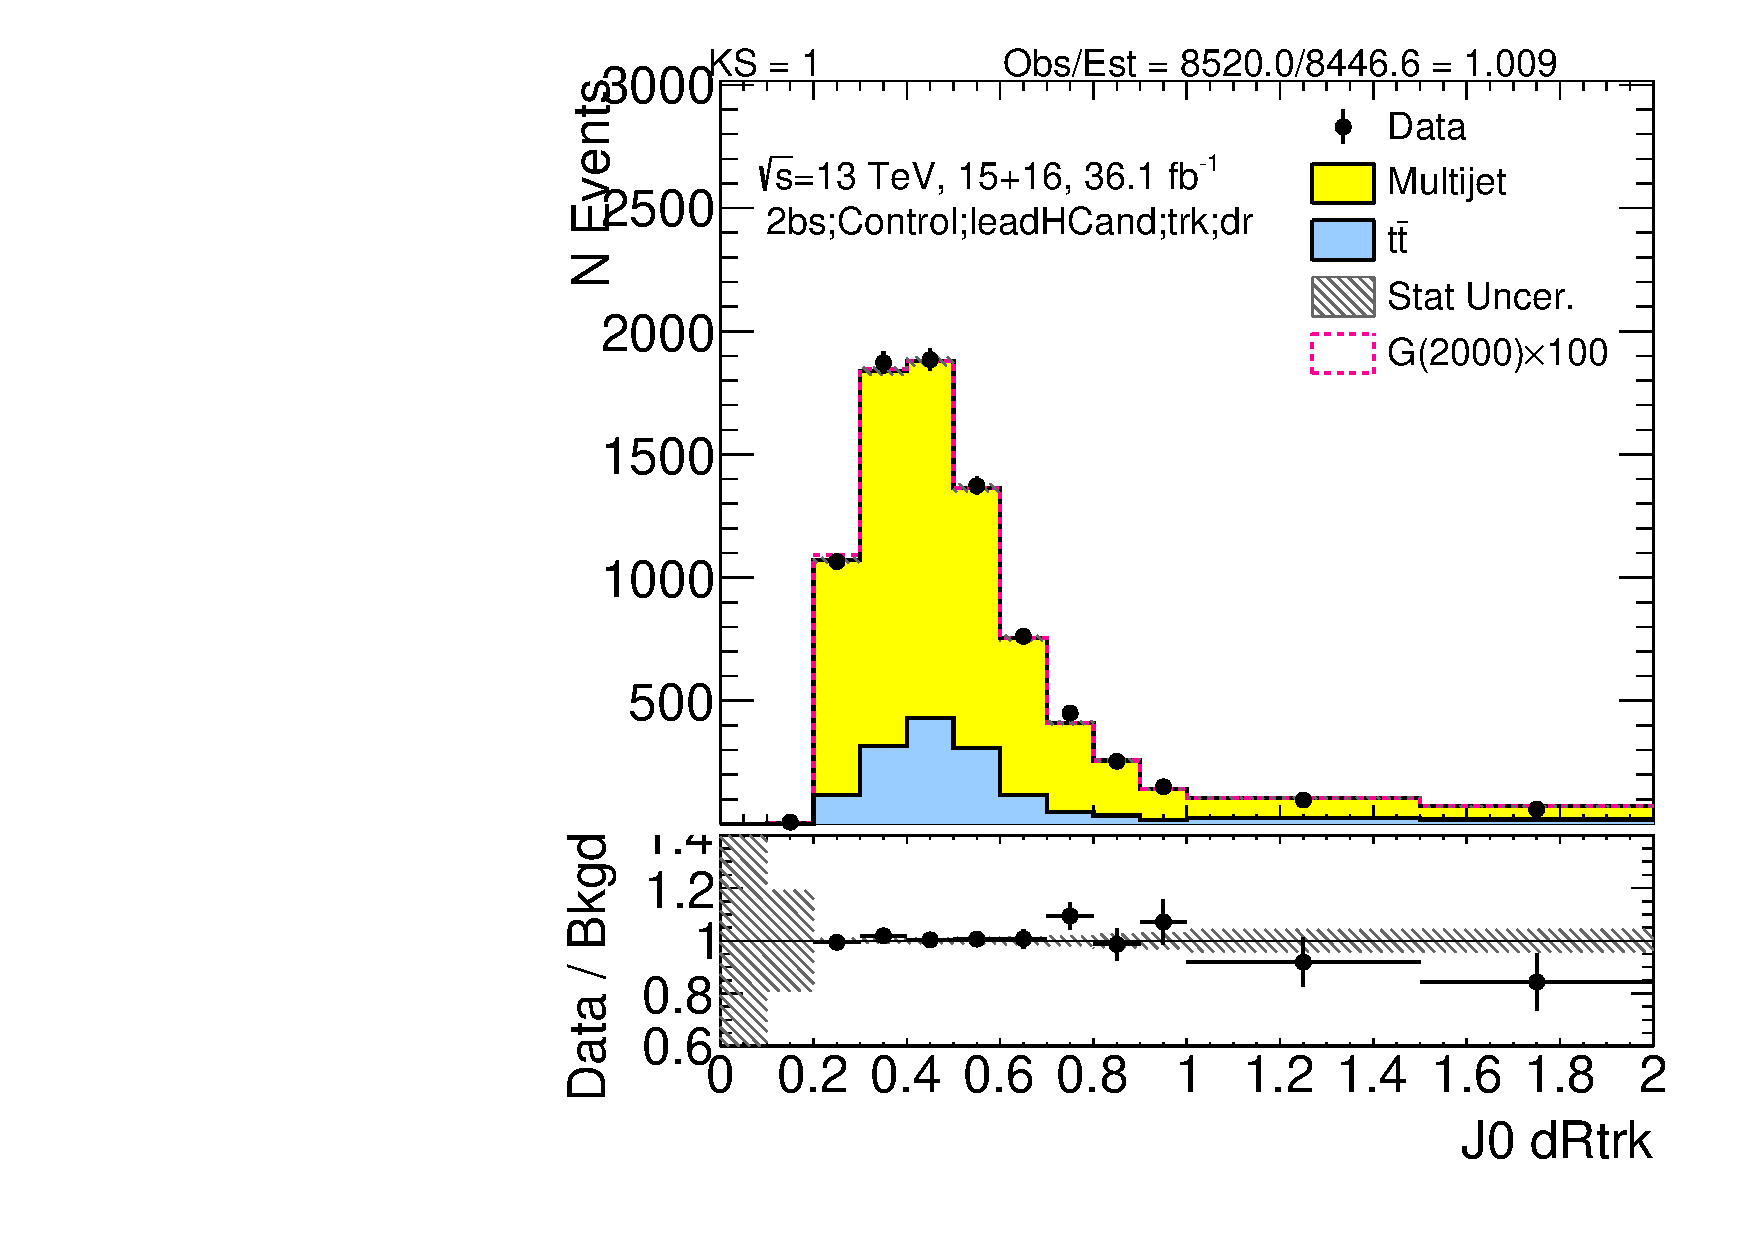
\includegraphics[width=0.33\textwidth, angle=270]{./figures/boosted/Control/Moriond_TwoTag_split_Control_leadHCand_trk_dr.pdf}
0.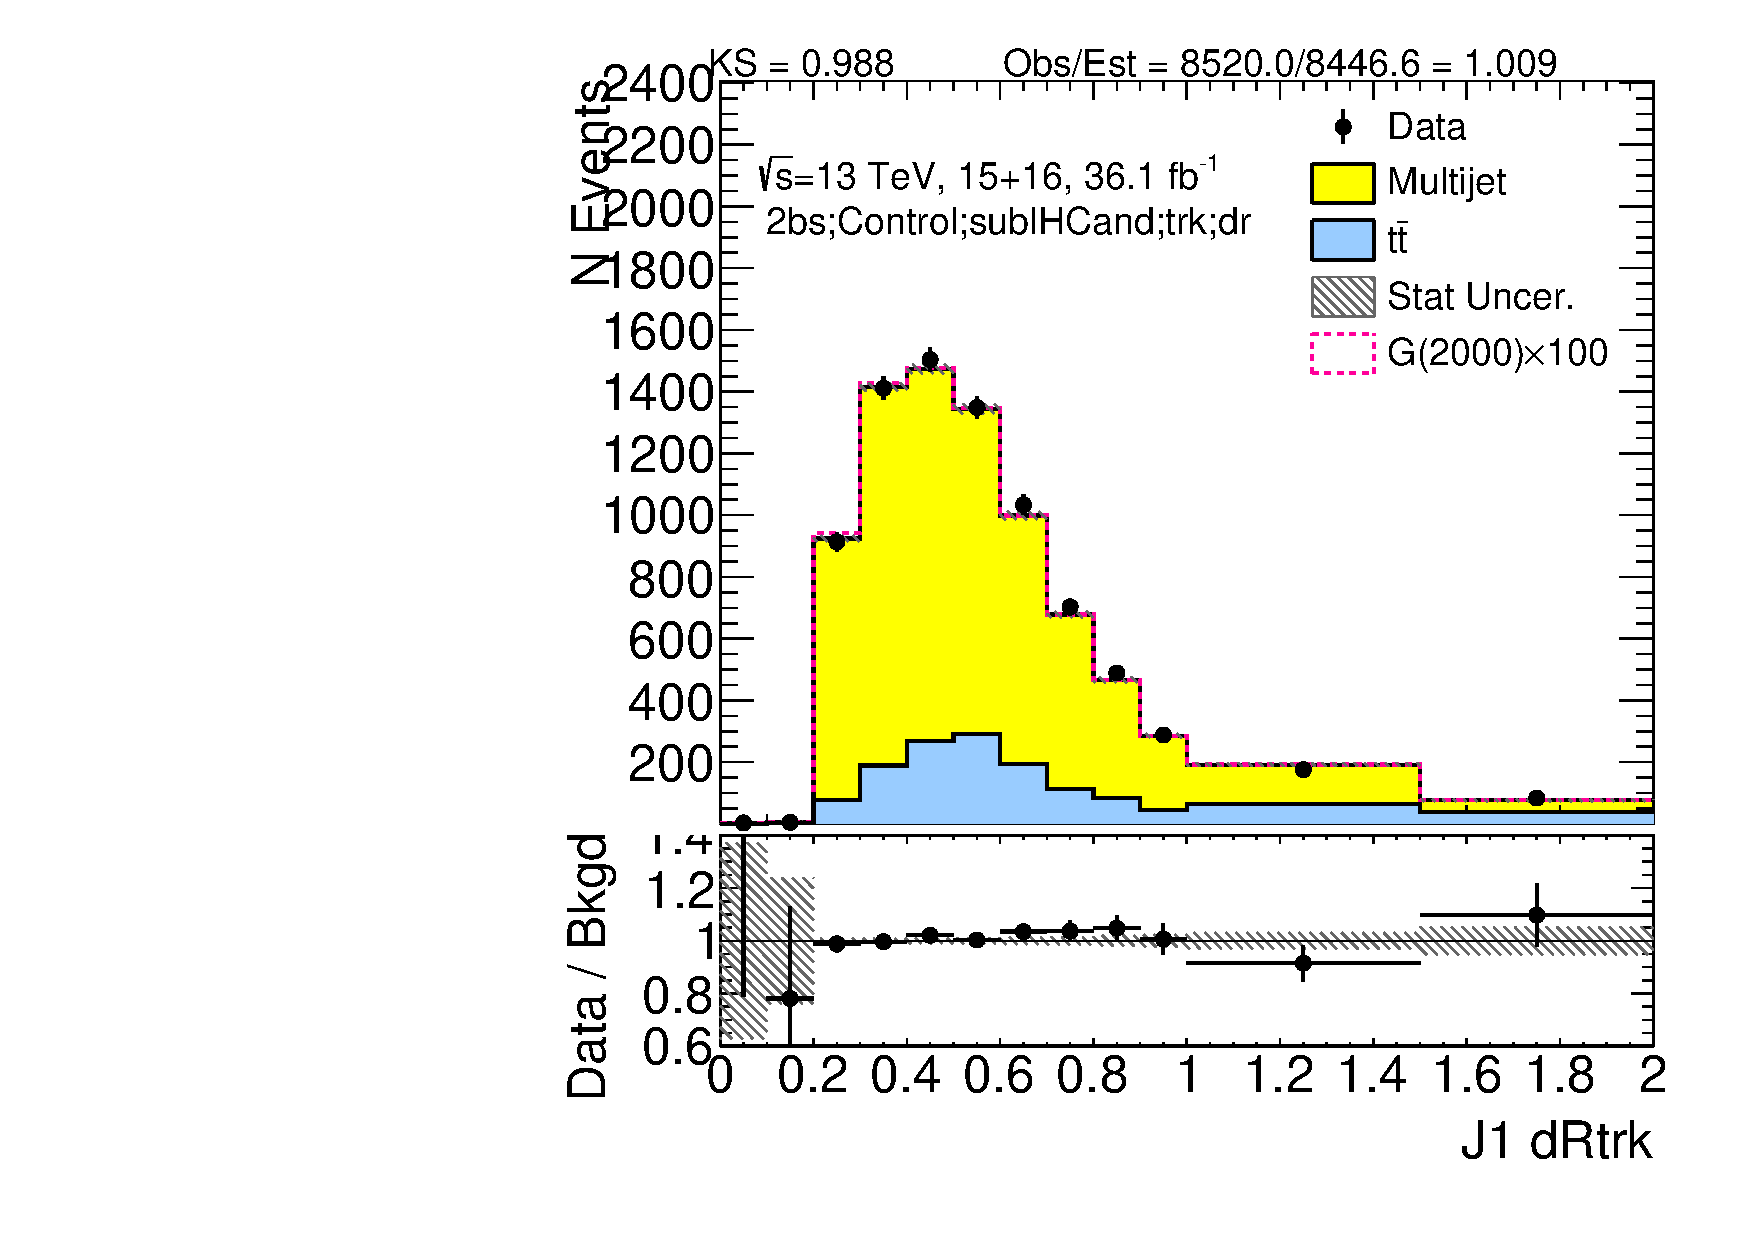
\includegraphics[width=0.33\textwidth, angle=270]{./figures/boosted/Control/Moriond_TwoTag_split_Control_sublHCand_trk_dr.pdf}
  \caption{First two rows show the kinematics of the lead (left) and sub-lead (right) small-$R$ track jets associated to the lead (first-row) and sub-lead (second-row) large-$R$ jet in data and prediction in the sideband region after requiring 2 $b$-tags split. Third row shows the $\Delta R$ between two leading small-$R$ track-jets associated to the leading (left) and sub-leading (right) large-$R$ jet. The normalization agrees by construction, and the shapes are a feature of the prediction. }
  \label{fig:boosted-2bs-control-ak2}
\end{center}
\end{figure*}


\begin{figure*}[htbp!]
\begin{center}
0.\includegraphics[width=0.33\textwidth, angle=270]{./figures/boosted/Control/Moriond_TwoTag_split_Control_mHH_l_1.pdf}
0.\includegraphics[width=0.33\textwidth, angle=270]{./figures/boosted/Control/Moriond_TwoTag_split_Control_hCandDr.pdf}\\
0.\includegraphics[width=0.33\textwidth, angle=270]{./figures/boosted/Control/Moriond_TwoTag_split_Control_hCandDeta.pdf}
0.\includegraphics[width=0.33\textwidth, angle=270]{./figures/boosted/Control/Moriond_TwoTag_split_Control_hCandDphi.pdf}
  \caption{Kinematics of the large-$R$ jet system in data and prediction in the sideband region after requiring 2 $b$-tags split. The normalization agrees by construction, and the shapes are a feature of the prediction. }
  \label{fig:boosted-2bs-control-ak10-system}
\end{center}
\end{figure*}




\section{Signal Region Predictions}

